\chapter{Appendix}
\label{ch:appendix}

\section{Sketches of Working Principles}
\label{appendix:sketches-of-working-principles}


\subsection{Screen Orientation}
\begin{table}[H]
    \centering
    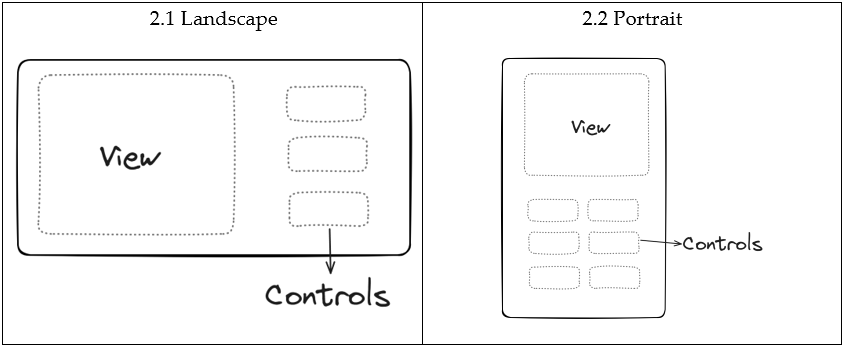
\includegraphics[width=\linewidth]{texs/Part1/chapter3/image/s2.png}
    \caption{Screen Orientation}
    \label{tab:screen-orientation}
\end{table}

\subsection{Battery Type}
\begin{table}[H]
    \centering
    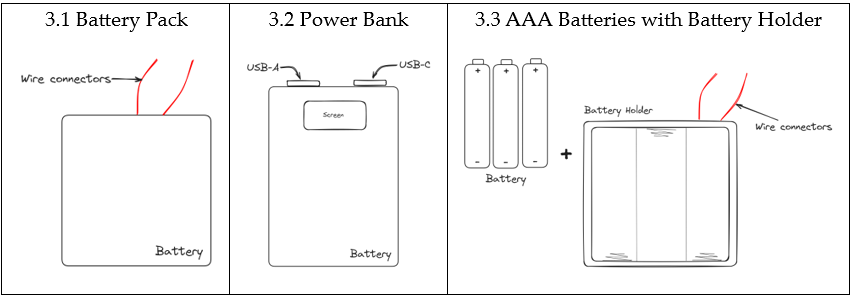
\includegraphics[width=\linewidth]{texs/Part1/chapter3/image/s3.png}
    \caption{Battery Type}
    \label{tab:battery-type}
\end{table}

\subsection{Components Placement}
\begin{table}[H]
    \centering
    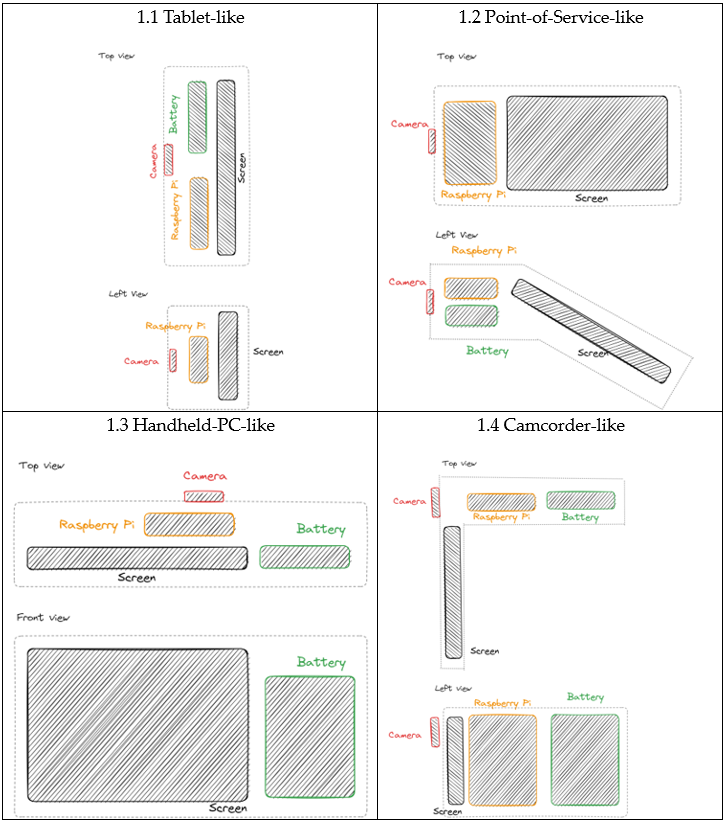
\includegraphics[width=\linewidth]{texs/Part1/chapter3/image/s1.png}
    \caption{Components Placement}
    \label{tab:components-placement}
\end{table}


\subsection{Body Type}
\begin{table}[H]
    \centering
    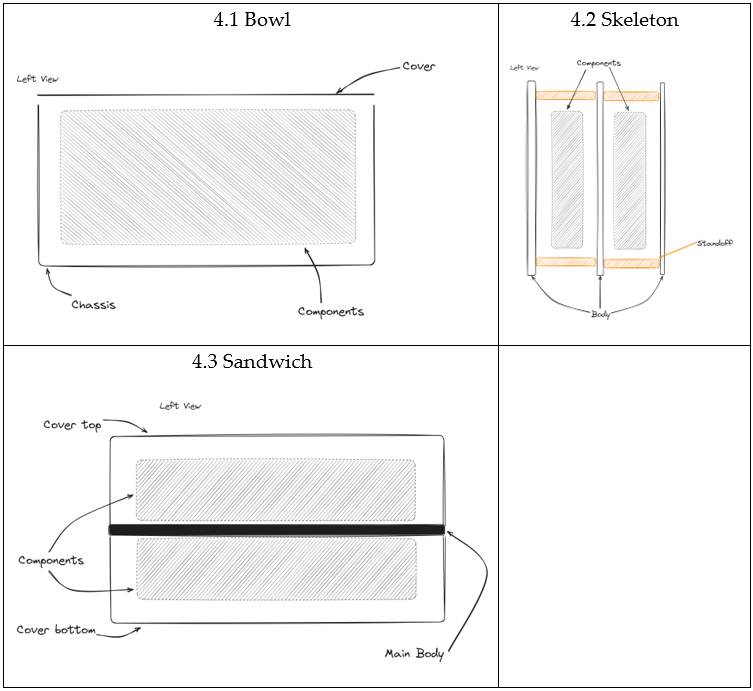
\includegraphics[width=\linewidth]{texs/Part1/chapter3/image/s4.png}
    \caption{Body Type}
    \label{tab:body-type}
\end{table}

\subsection{Handling}
\begin{table}[H]
    \centering
    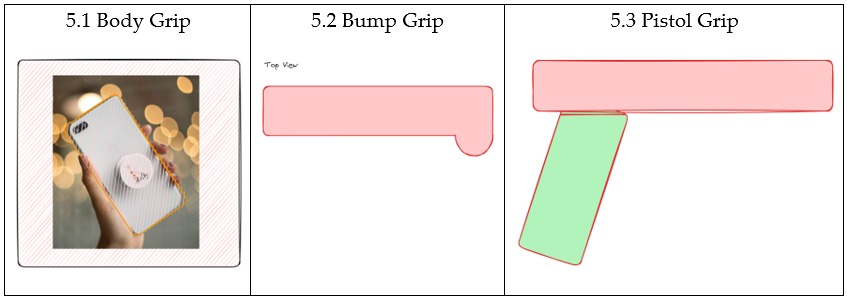
\includegraphics[width=\linewidth]{texs/Part1/chapter3/image/s5.png}
    \caption{Handling}
    \label{tab:handling}
\end{table}

\subsection{External Mounting}
\begin{table}[H]
    \centering
    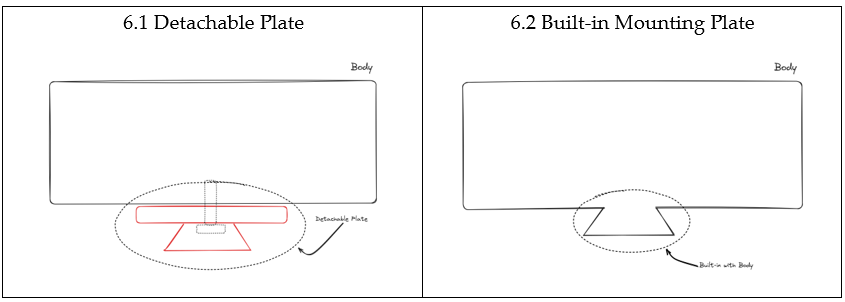
\includegraphics[width=\linewidth]{texs/Part1/chapter3/image/s6.png}
    \caption{External Mounting}
    \label{tab:external-mounting}
\end{table}

\subsection{Control Mechanism}
\begin{table}[H]
    \centering
    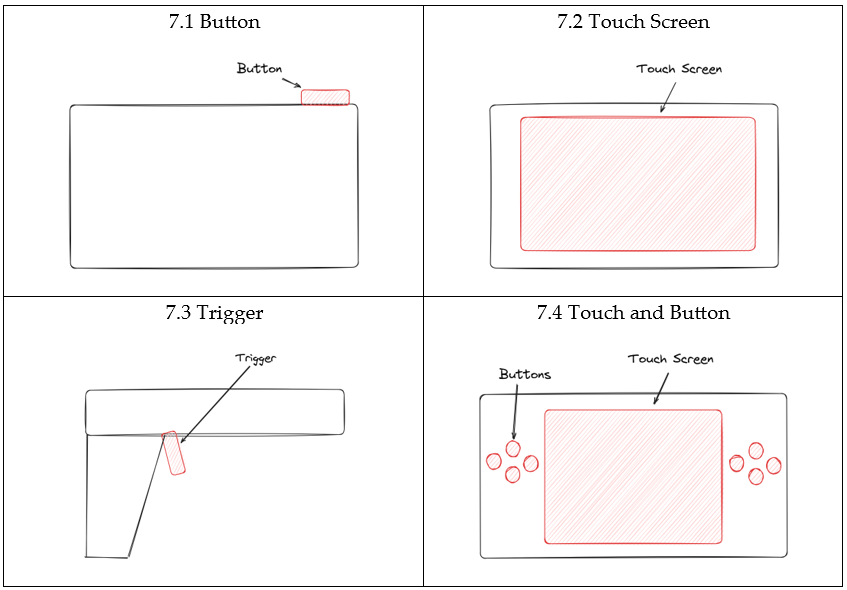
\includegraphics[width=\linewidth]{texs/Part1/chapter3/image/s7.png}
    \caption{Control Mechanism}
    \label{tab:control-mechanism}
\end{table}

\section{CAD Drawings}
\label{appendix:cad-drawings}

\begin{figure}[H]
    \centering
    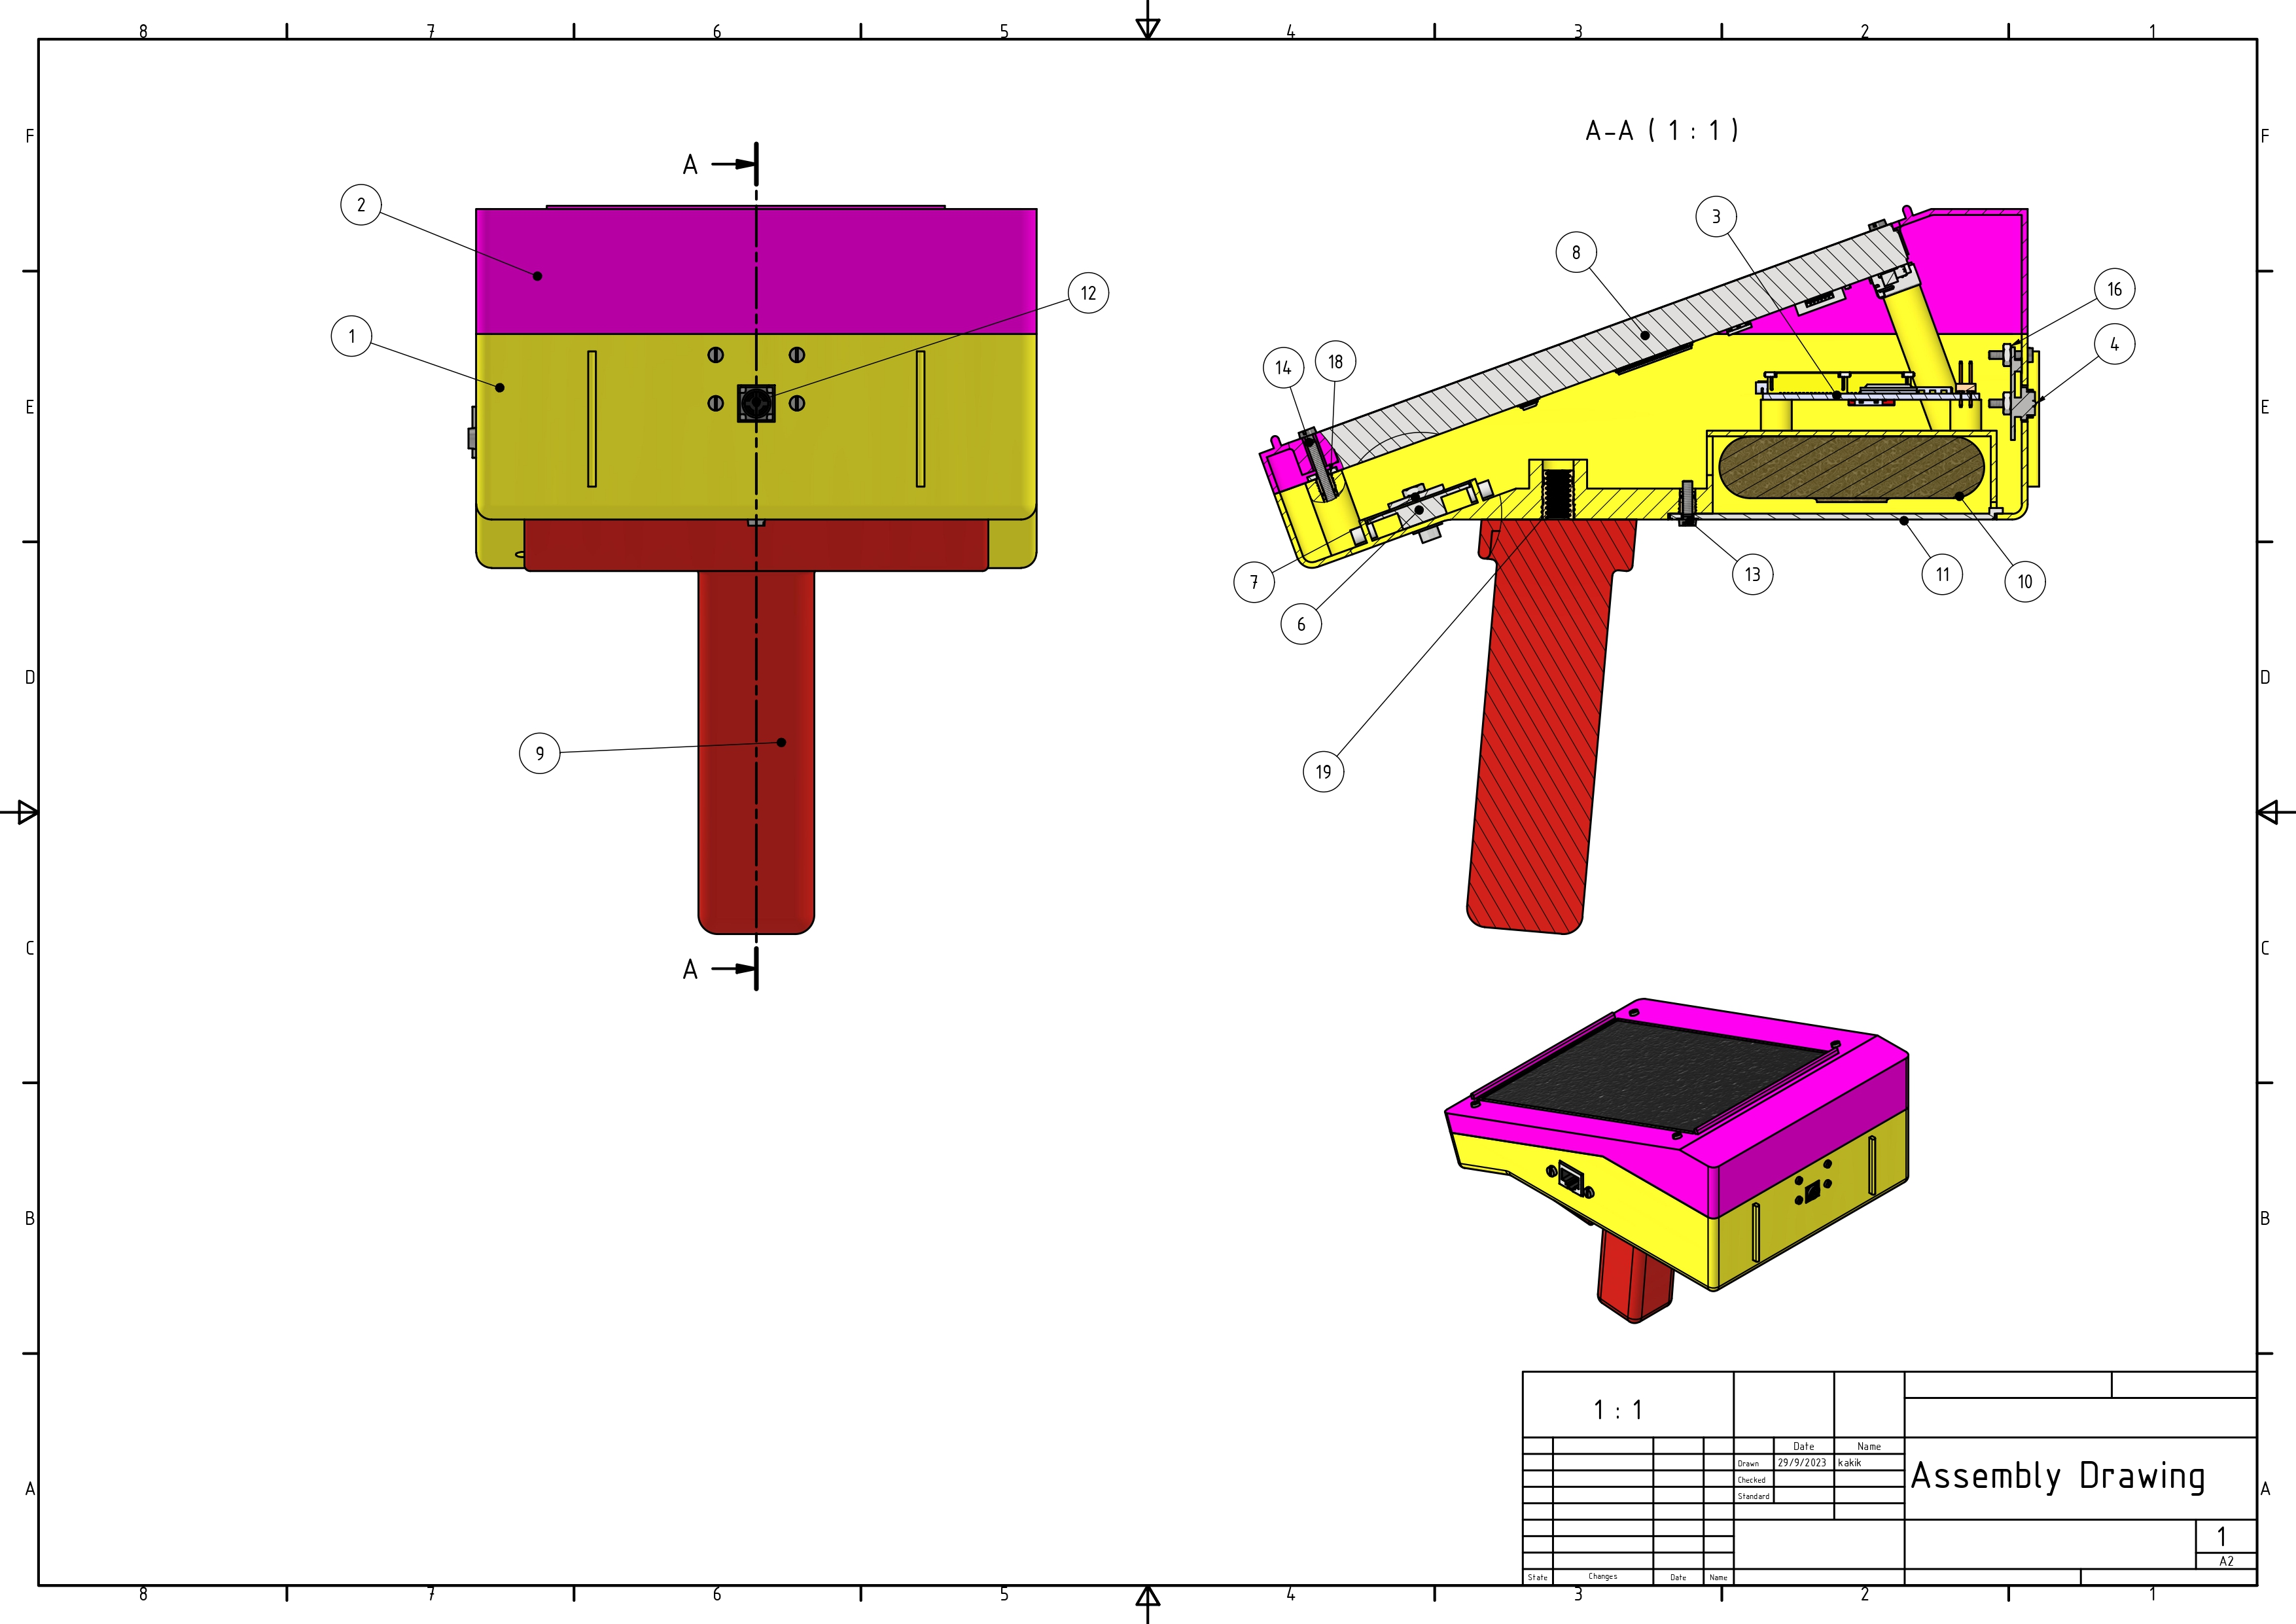
\includegraphics[width=1.2\linewidth, angle = 90]{texs/appendix/data/technicaldrawing/assembly.jpg}
    \caption{Assembly Drawing}
    \label{fig:cad-drawing-assembly}
\end{figure}

\begin{figure}[H]
    \centering
    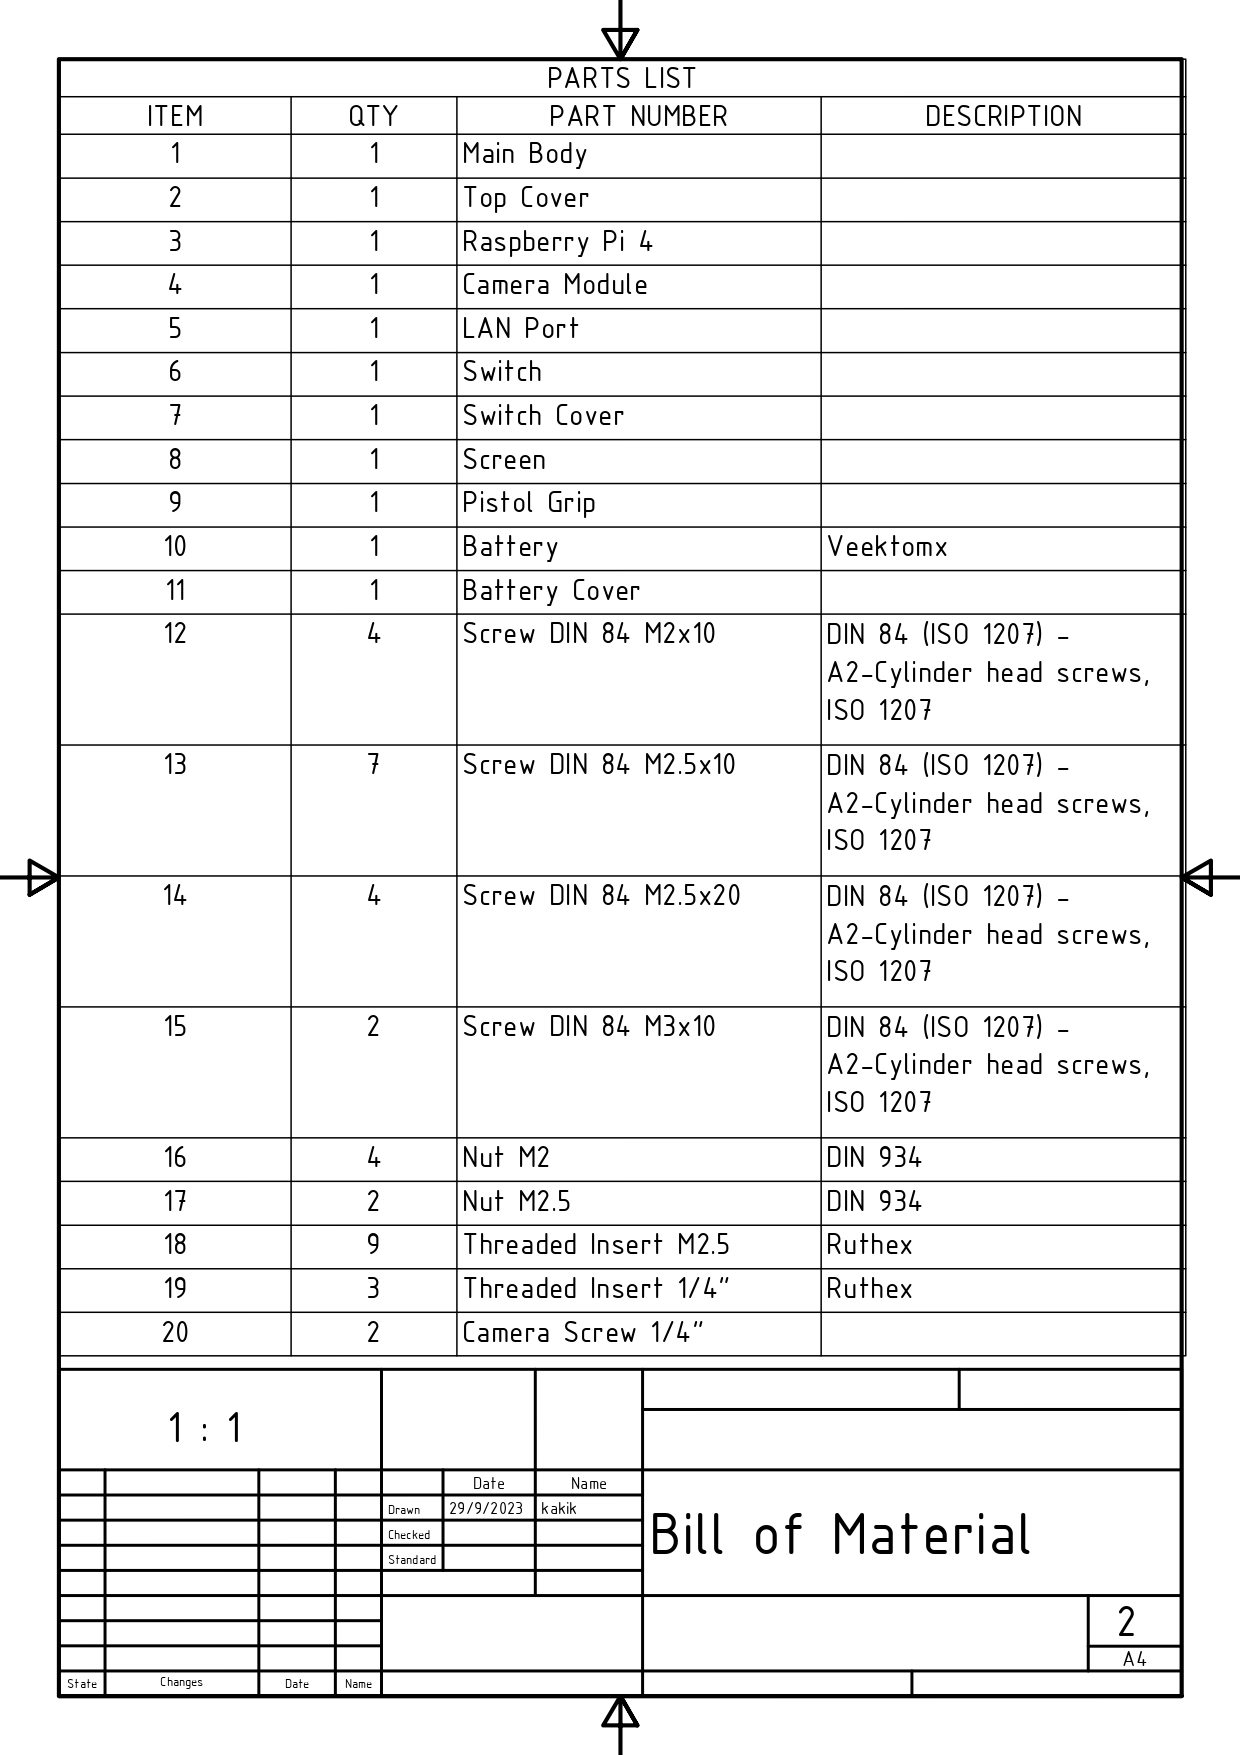
\includegraphics[width=0.9\linewidth]{texs/appendix/data/technicaldrawing/bom.jpg}
    \caption{Bill of Materials}
    \label{fig:cad-drawing-bom}
\end{figure}

\begin{figure}[H]
    \centering
    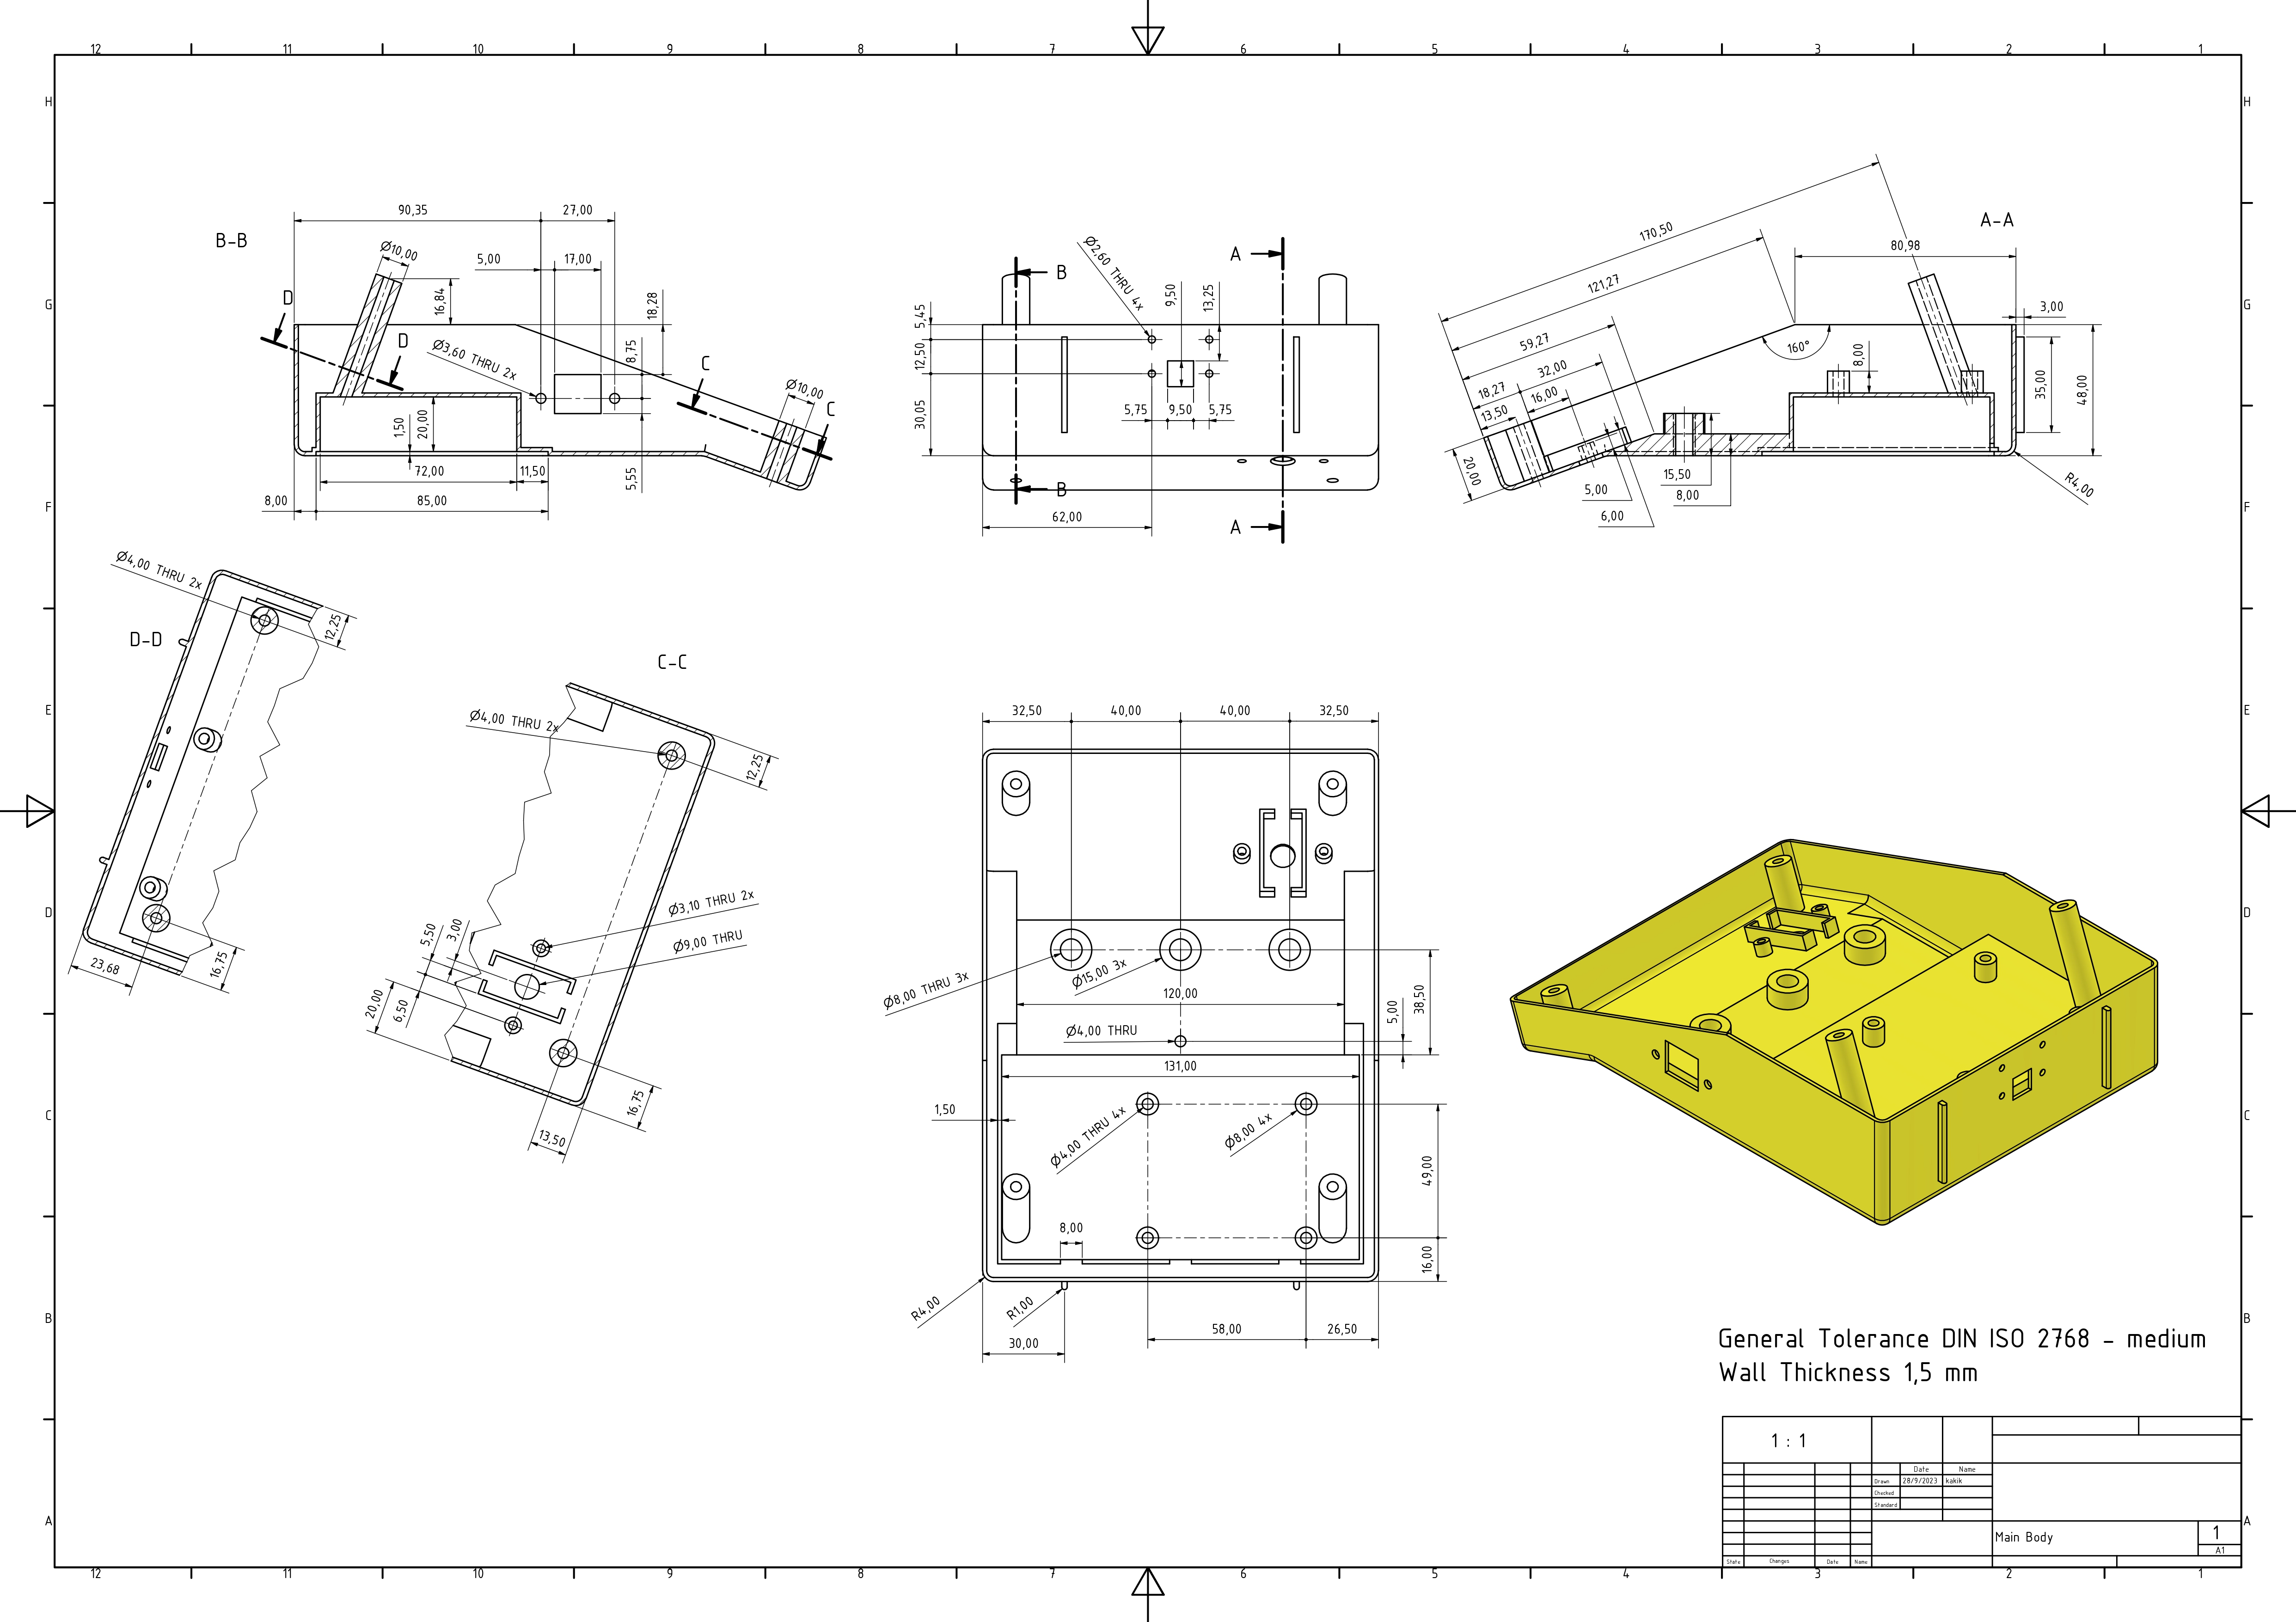
\includegraphics[width=1.3\linewidth, angle = 90]{texs/appendix/data/technicaldrawing/mainbody.jpg}
    \caption{Main Body Drawing}
    \label{fig:cad-drawing-mainbody}
\end{figure}

\begin{figure}[H]
    \centering
    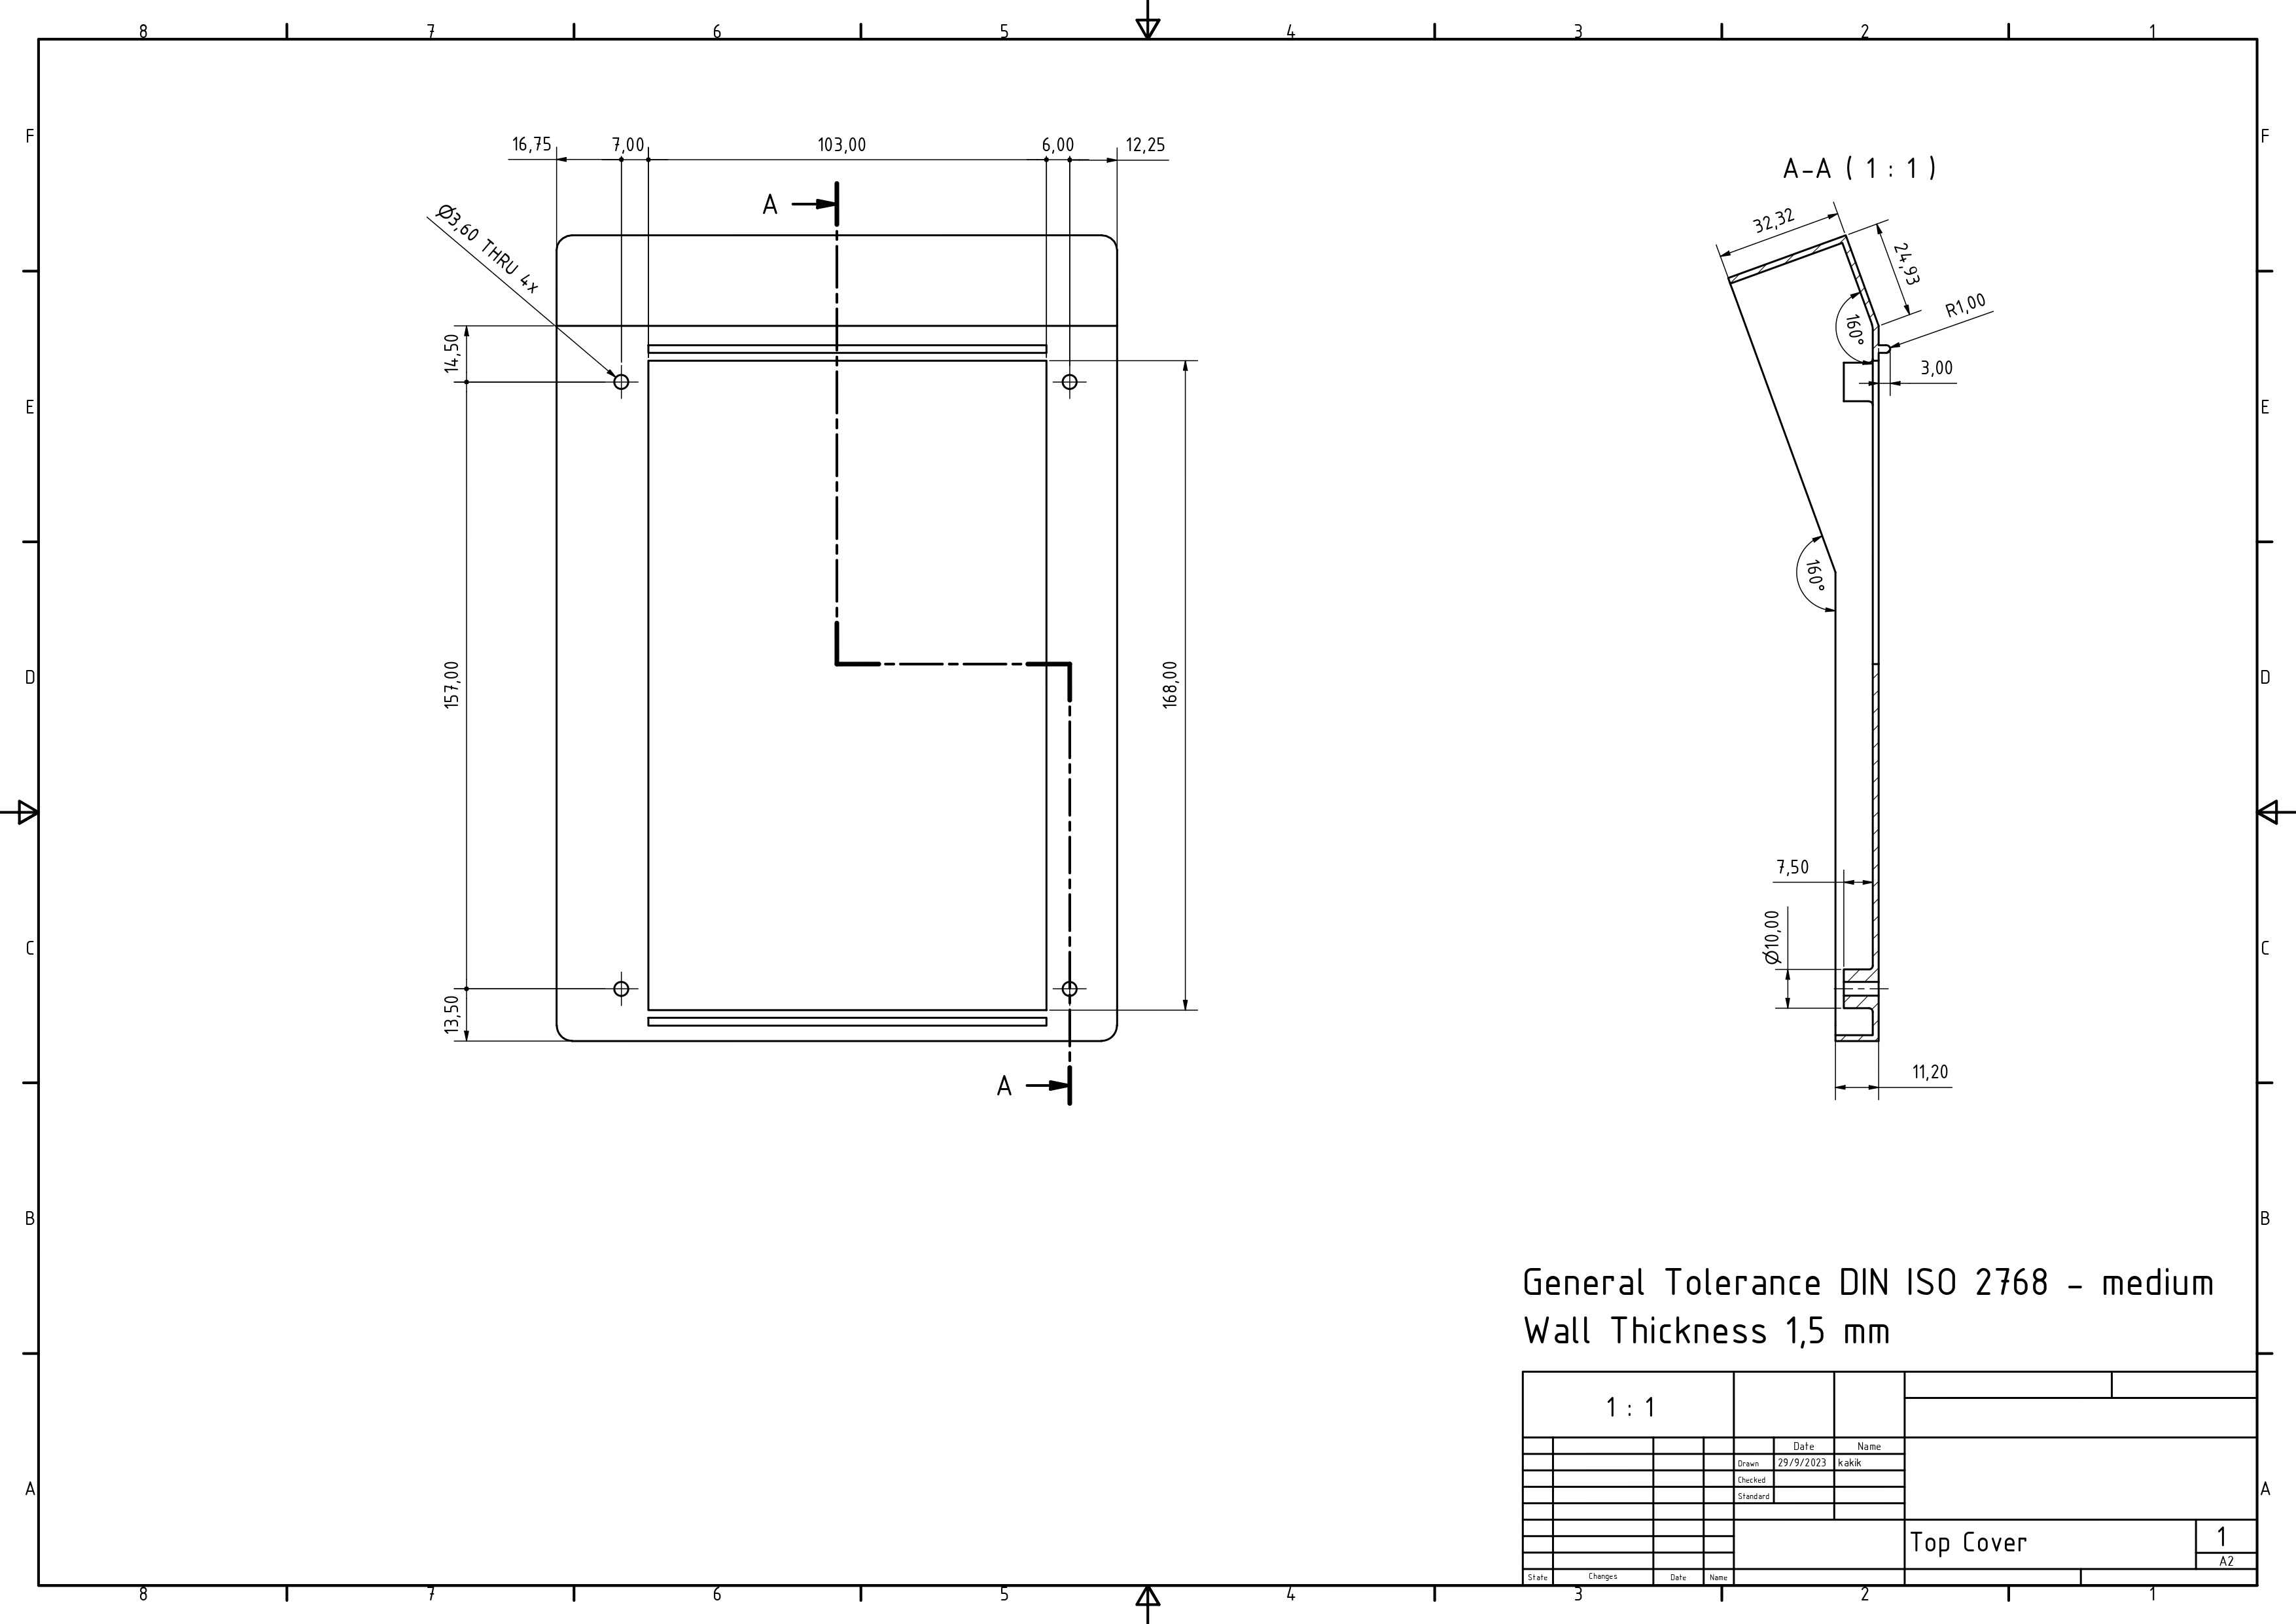
\includegraphics[width=1.3\linewidth, angle = 90]{texs/appendix/data/technicaldrawing/topcover.jpg}
    \caption{Top Cover Drawing}
    \label{fig:cad-drawing-topcover}
\end{figure}

\begin{figure}[H]
    \centering
    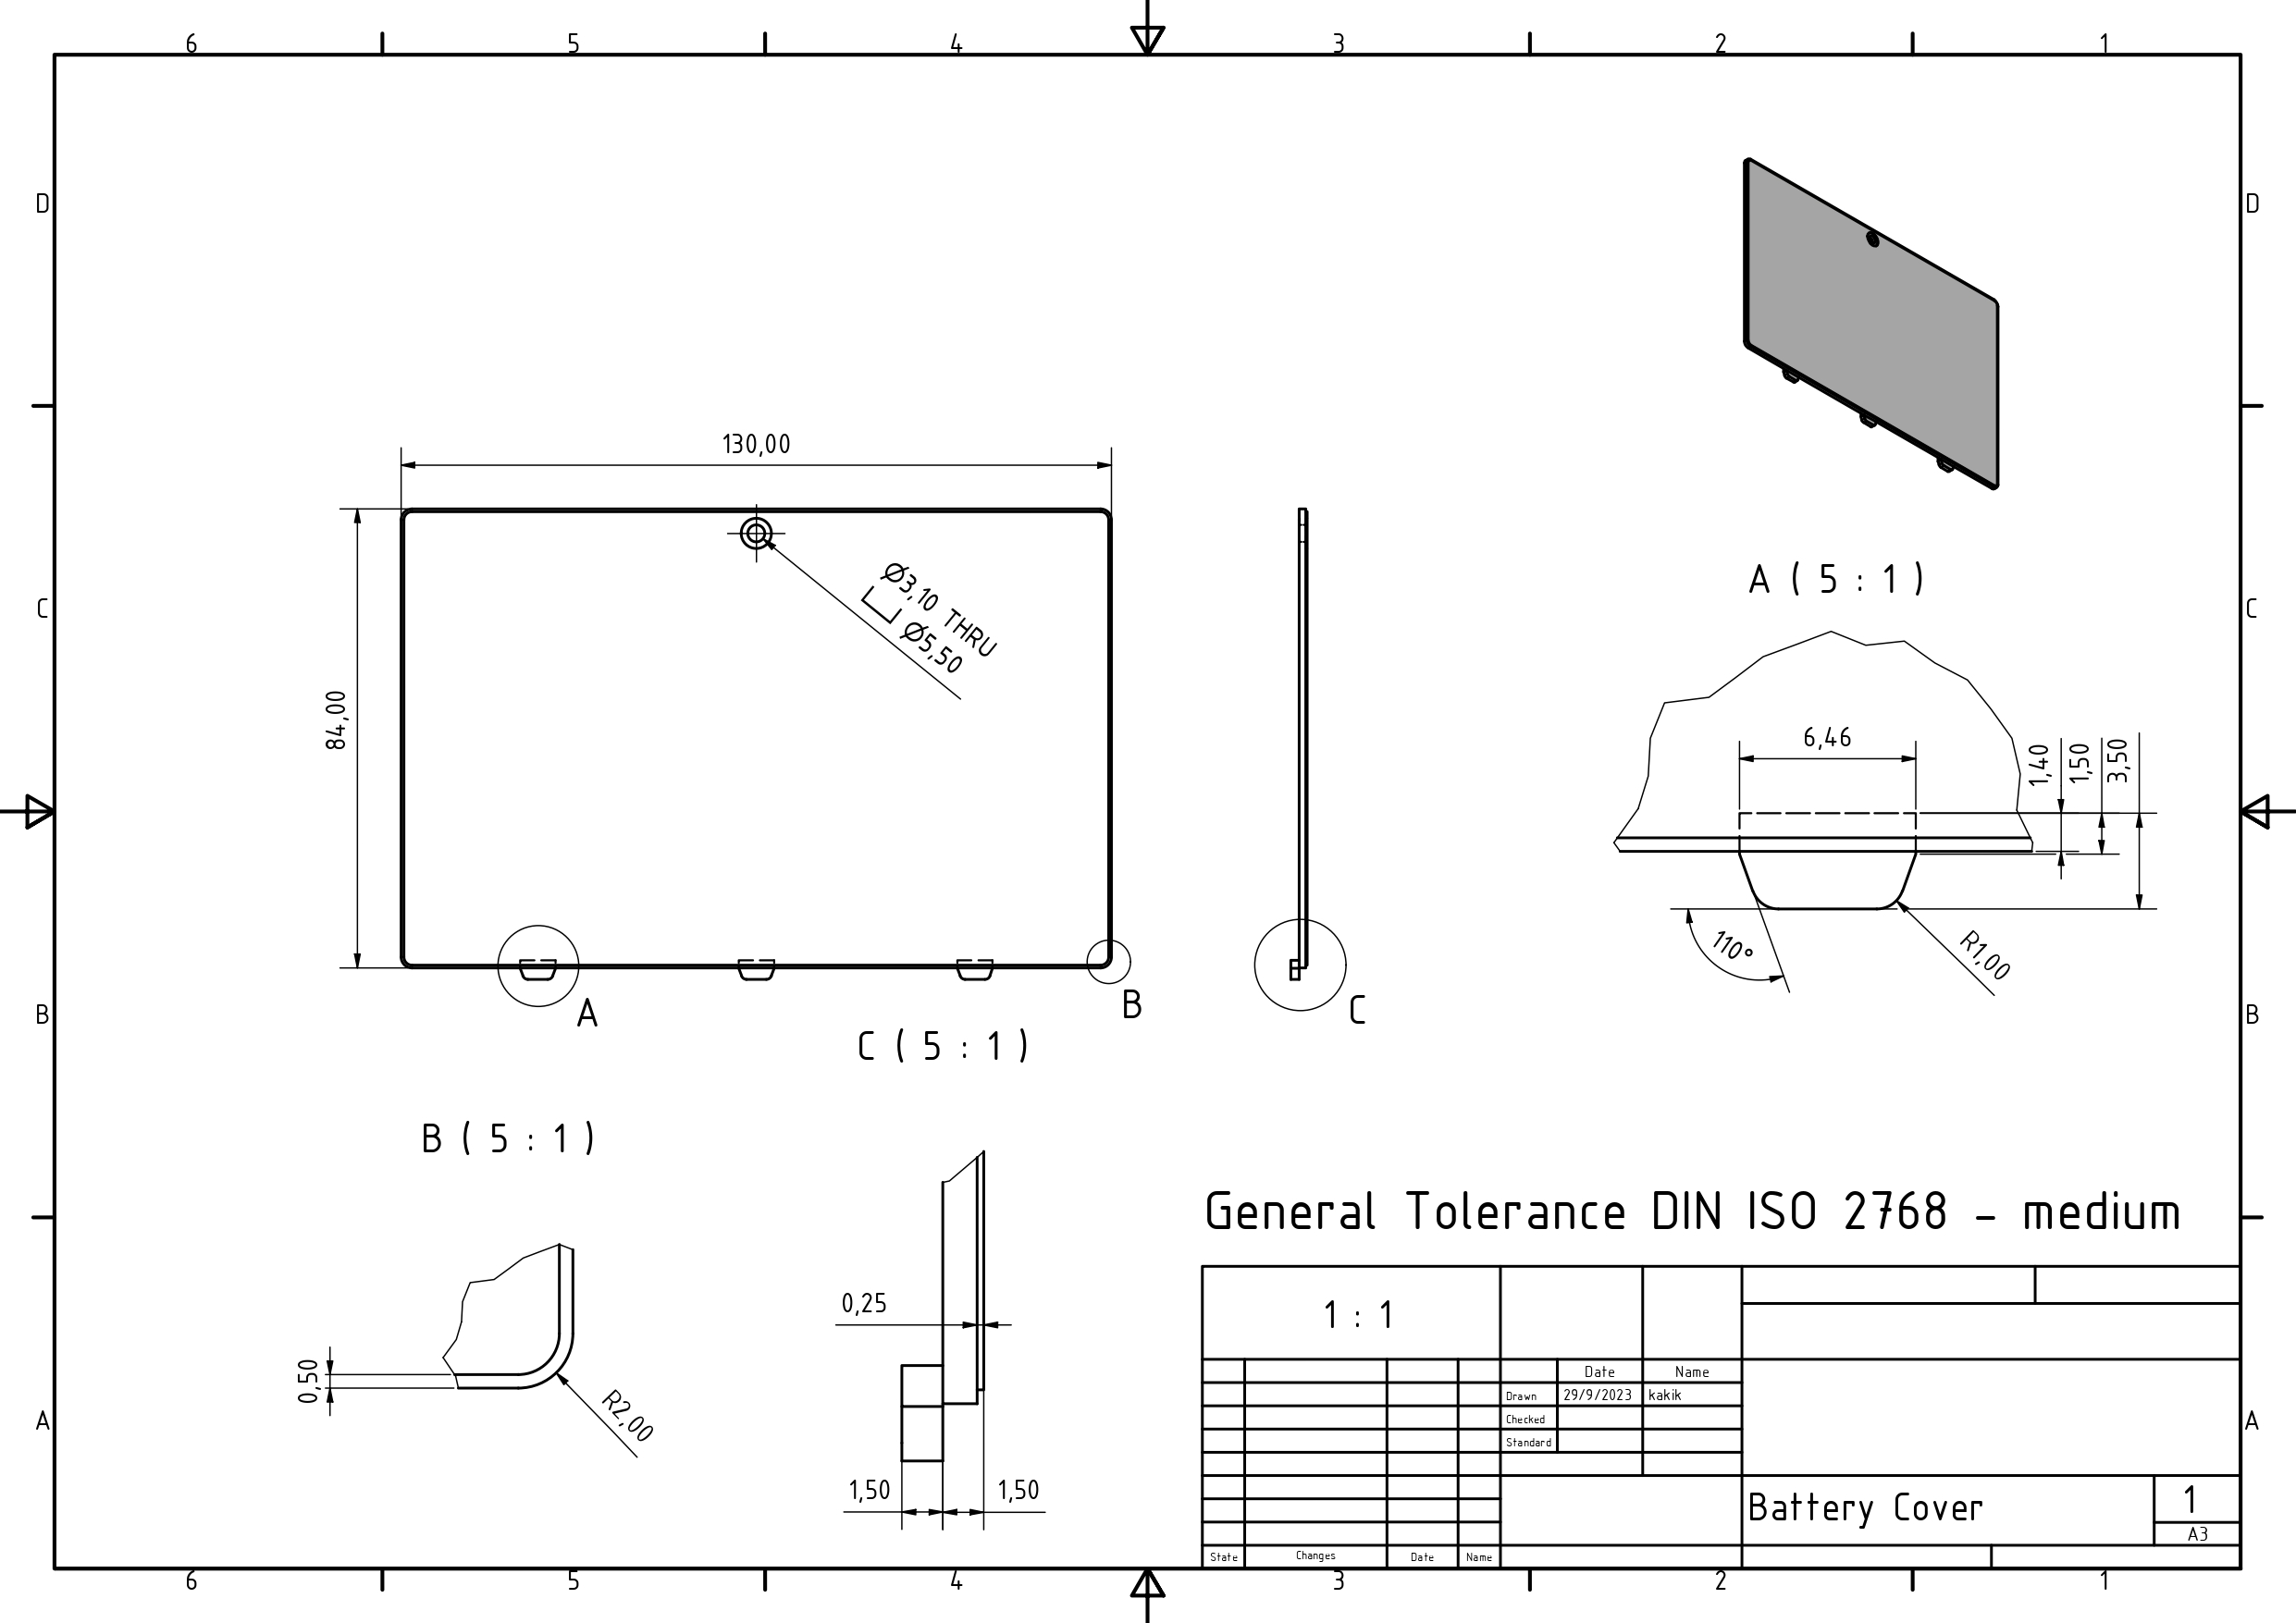
\includegraphics[width=1.3\linewidth, angle = 90]{texs/appendix/data/technicaldrawing/batterycover.jpg}
    \caption{Battery Cover Drawing}
    \label{fig:cad-drawing-batterycover}
\end{figure}

\begin{figure}[H]
    \centering
    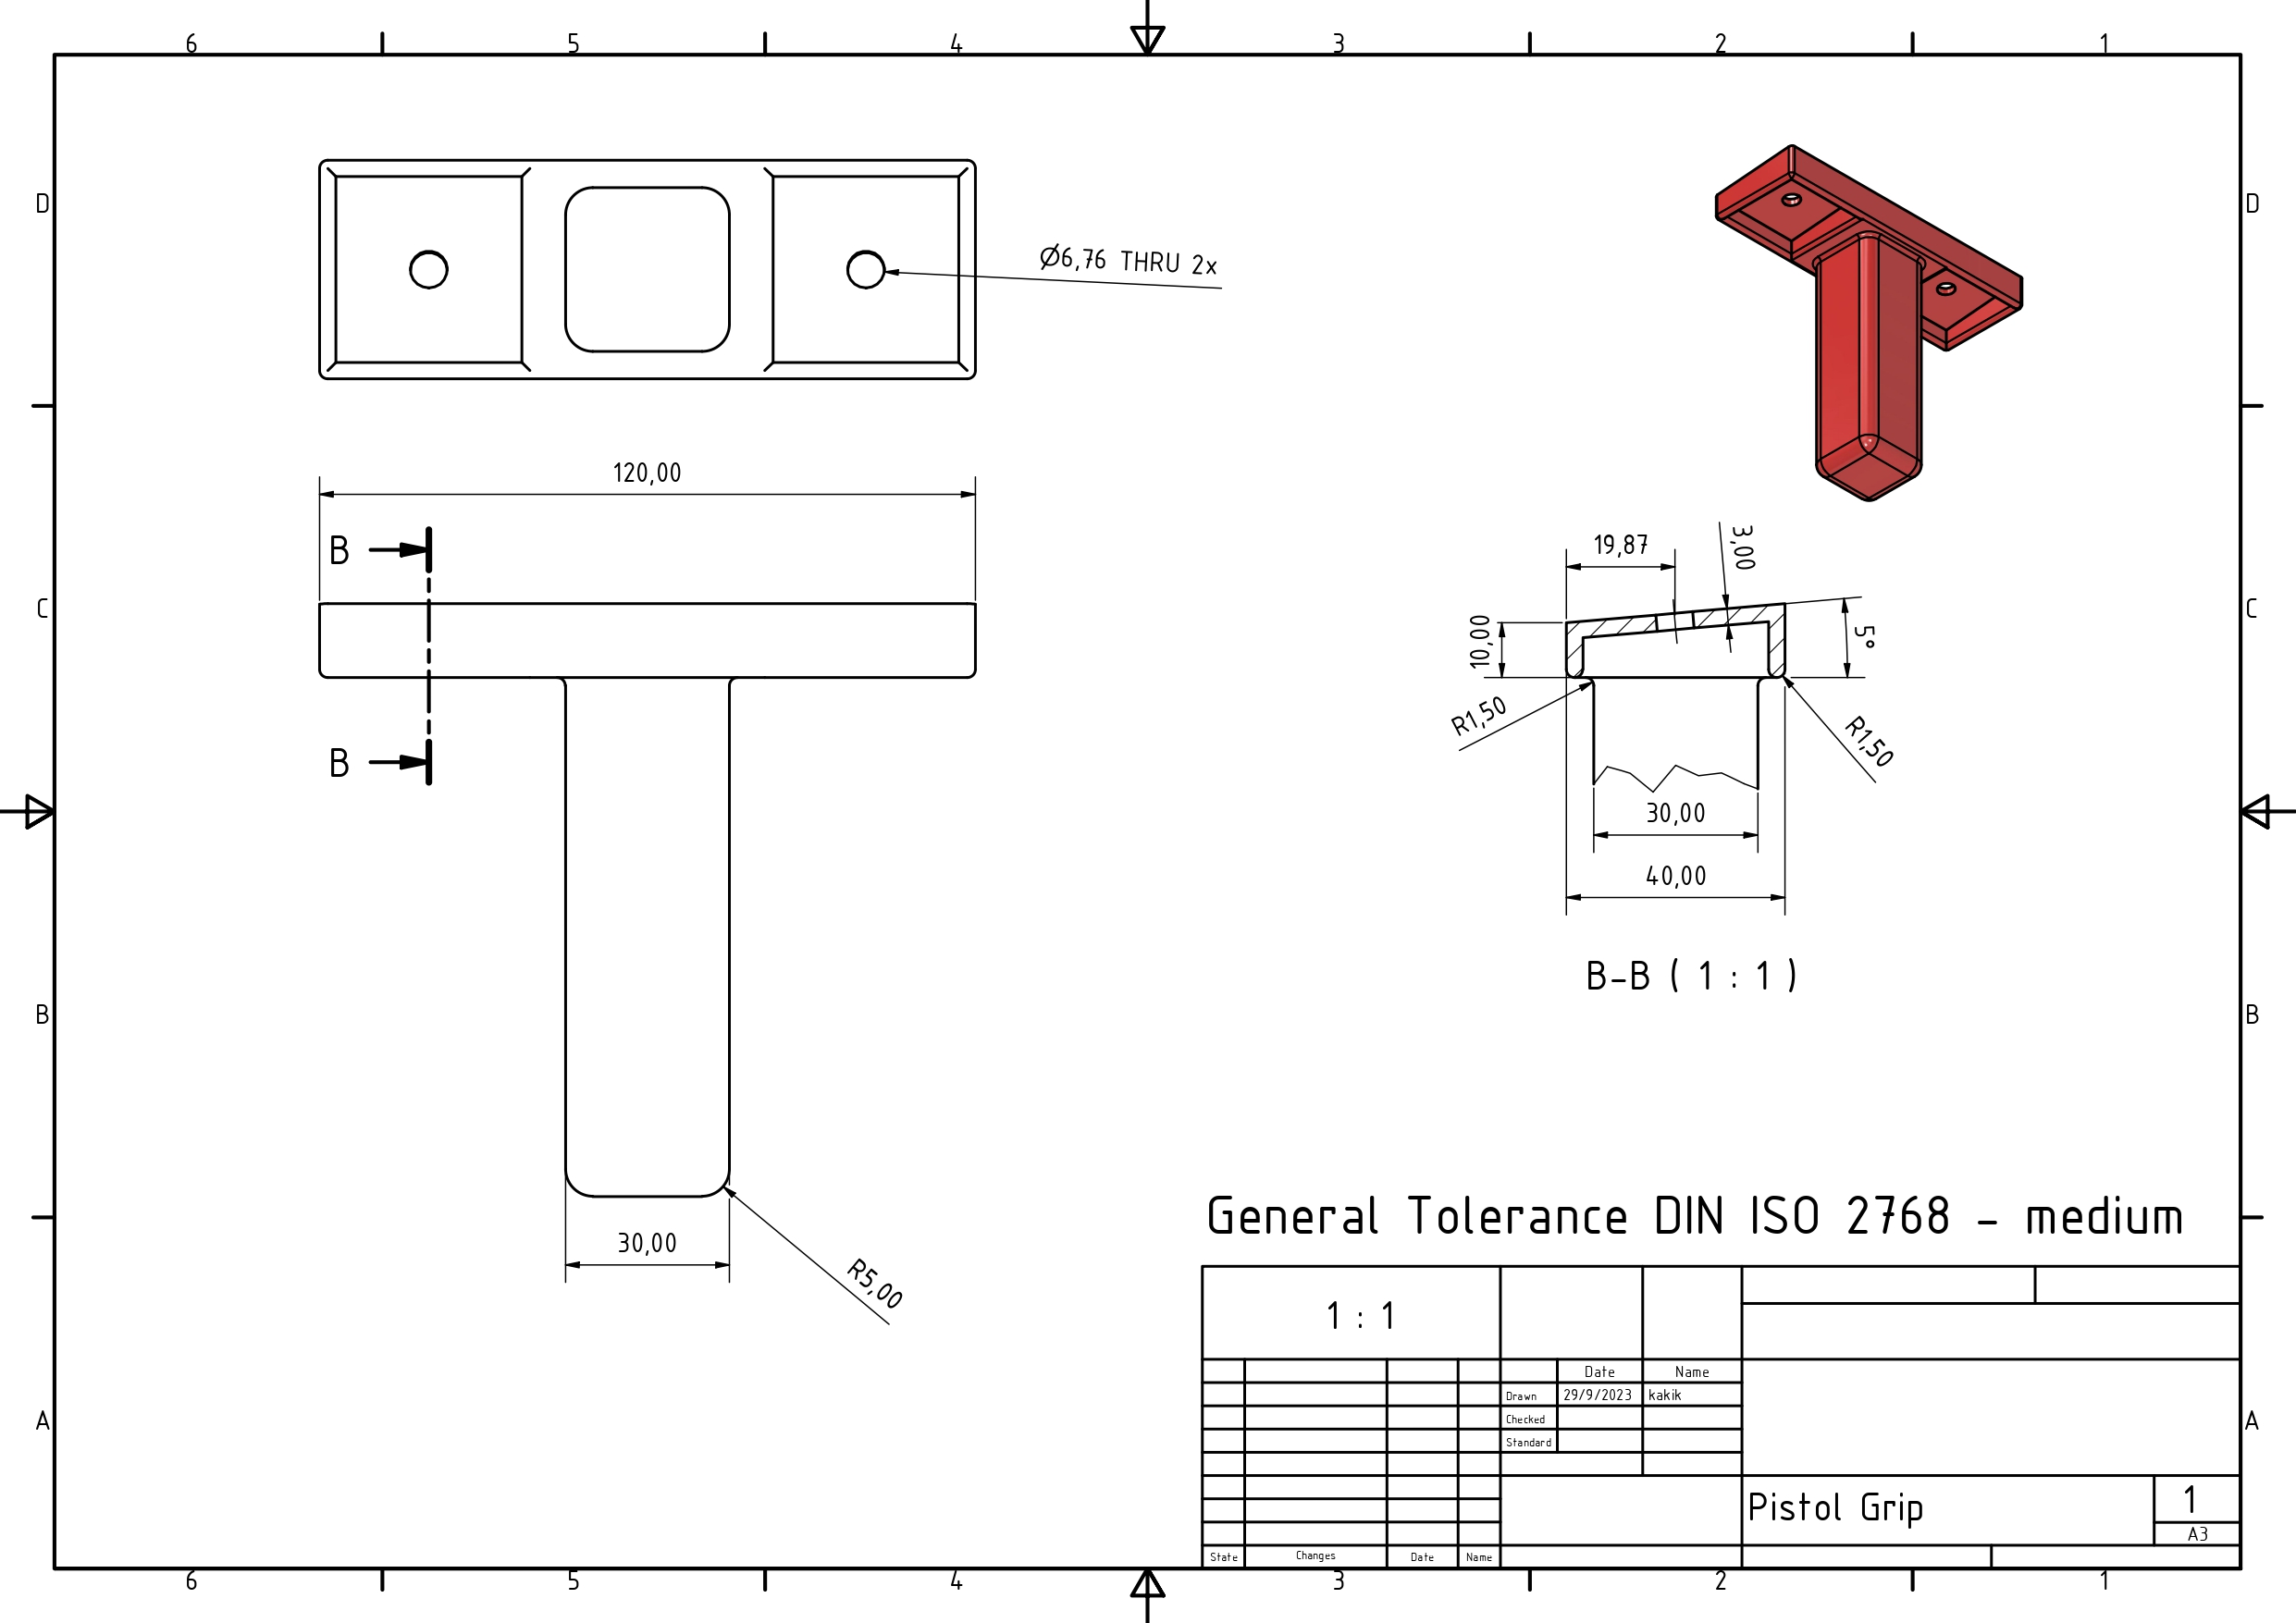
\includegraphics[width=1.3\linewidth, angle = 90]{texs/appendix/data/technicaldrawing/pistolgrip.jpg}
    \caption{Pistol Grip Drawing}
    \label{fig:cad-drawing-pistolgrip}
\end{figure}

\begin{figure}[H]
    \centering
    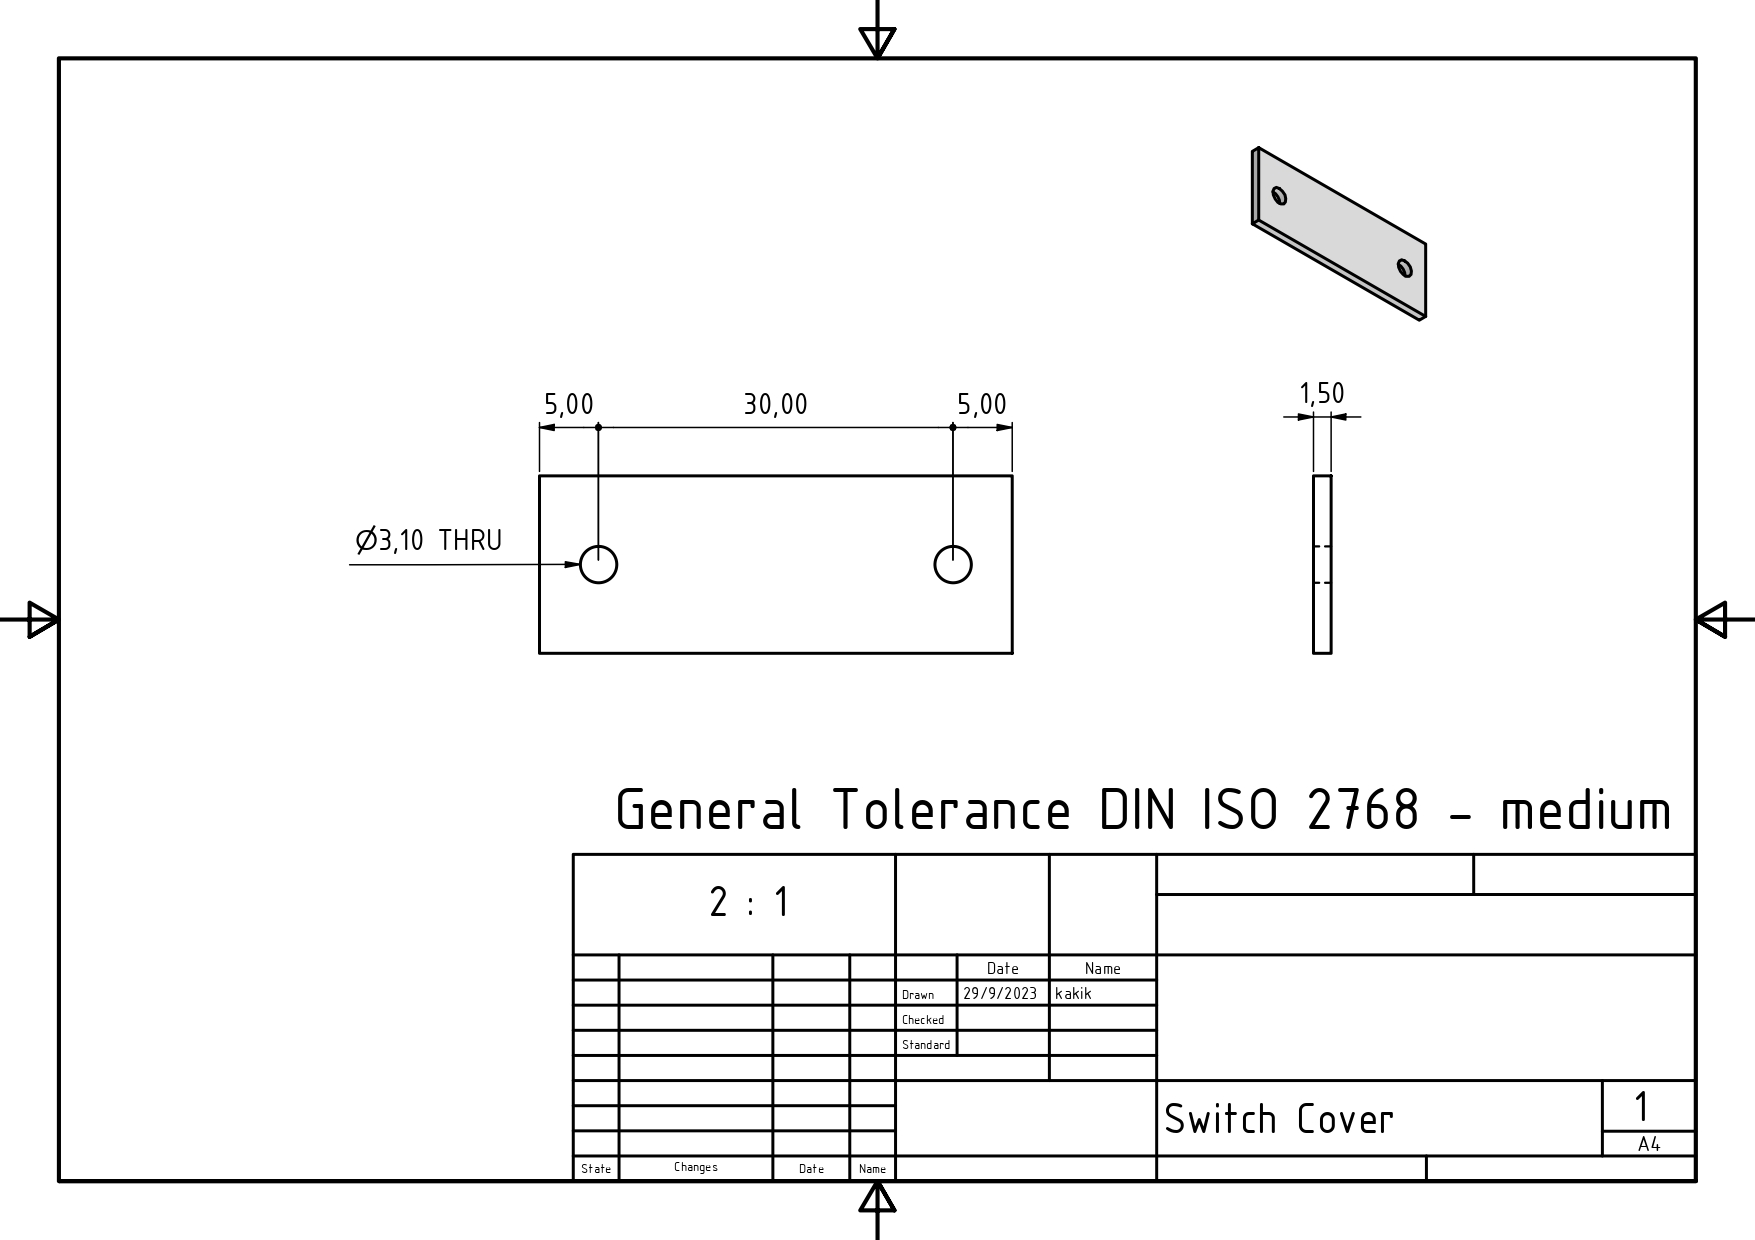
\includegraphics[width=1.3\linewidth, angle = 90]{texs/appendix/data/technicaldrawing/switchcover.jpg}
    \caption{Switch Cover Drawing}
    \label{fig:cad-drawing-switchcover}
\end{figure}

\section{Technical Specifications}
\subsection{Original Prusa i3 MK3S+ 3D printer}
\label{appendix:original-prusa-i3-mk3s-3d-printer}

\begin{figure}[H]
    \centering
    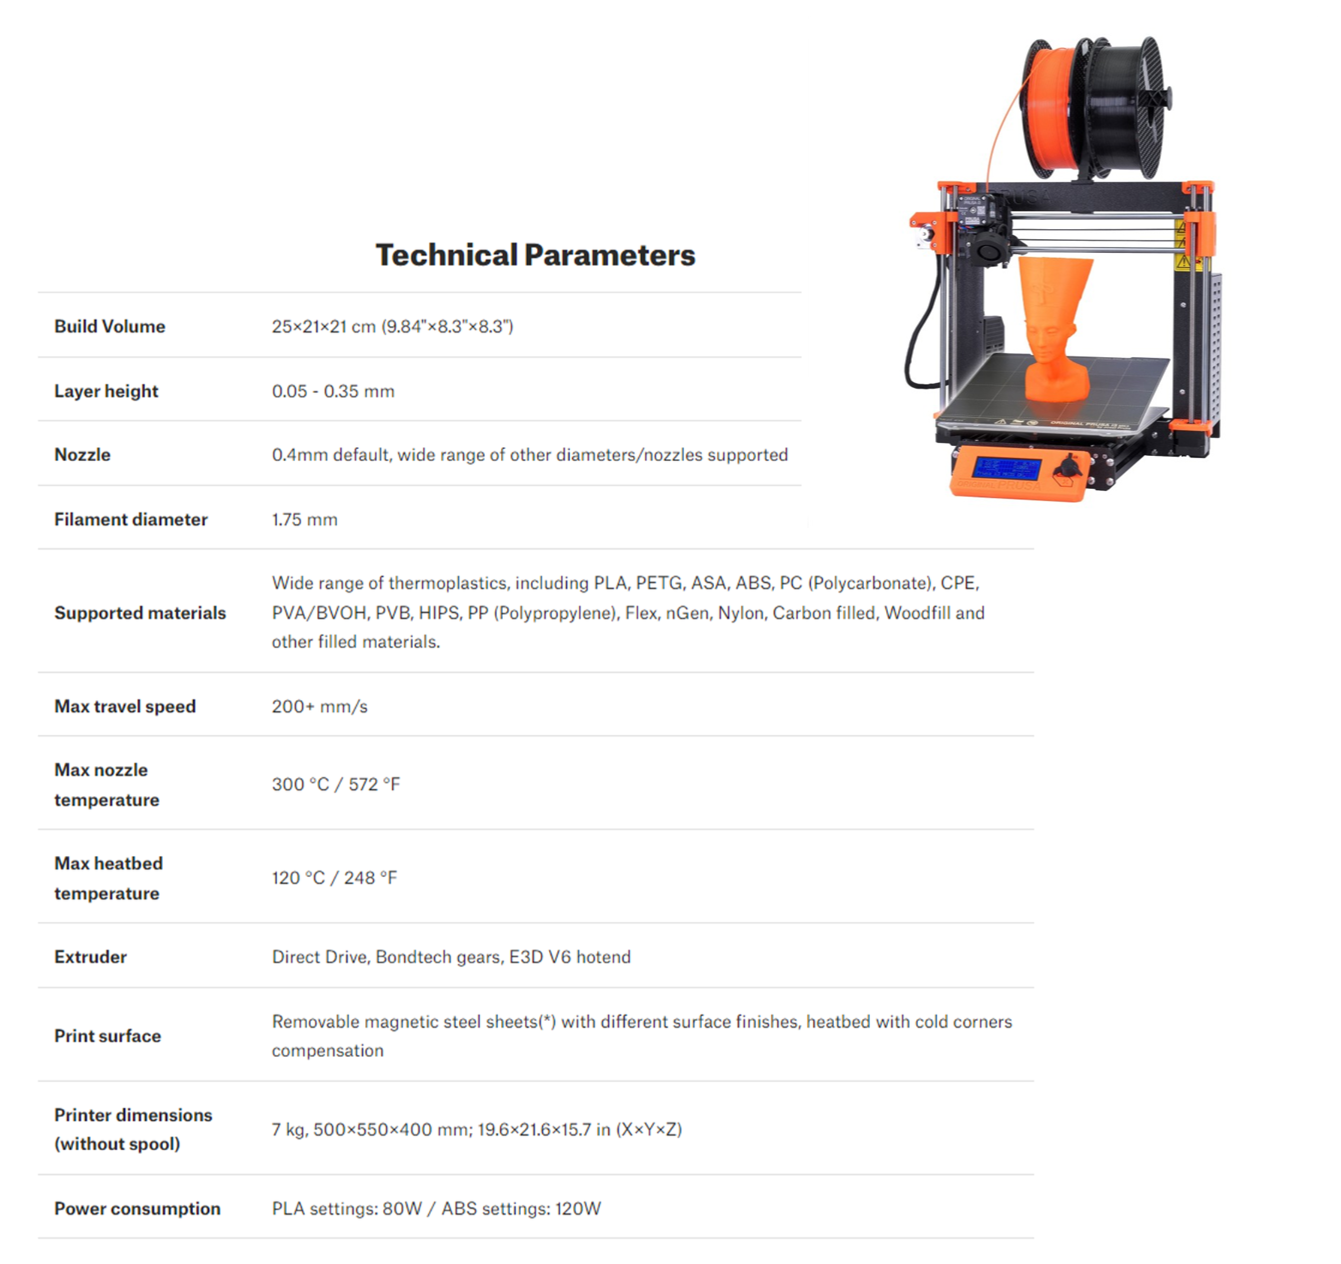
\includegraphics[width=\linewidth]{texs/appendix/data/techspecs/prusa.png}
    \caption{Original Prusa i3 MK3S+ 3D printer}
    \label{fig:3d-printer-1}
\end{figure}

\subsection{Raspberry Pi 4 Model B}
\label{appendix:raspberry-pi-4-model-b}

\begin{figure}[H]
    \centering
    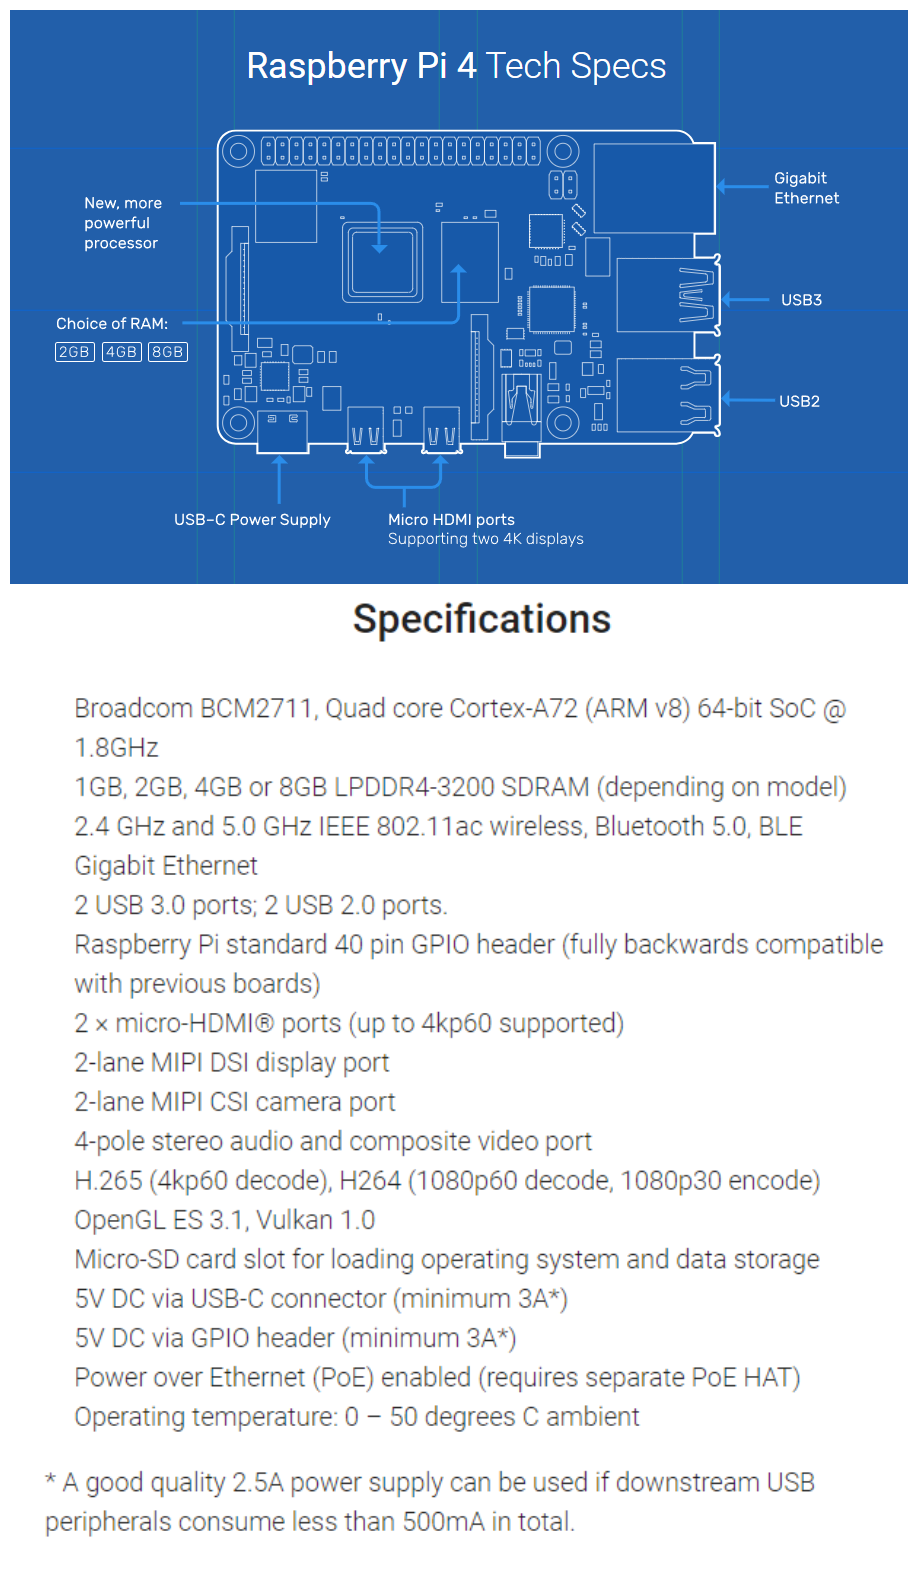
\includegraphics[width=0.7\linewidth]{texs/appendix/data/techspecs/pi-specs.png}
    \caption{Raspberry Pi 4 Model B Technical Specifications}
    \label{fig:rpi-1}
\end{figure}

\begin{figure}[H]
    \centering
    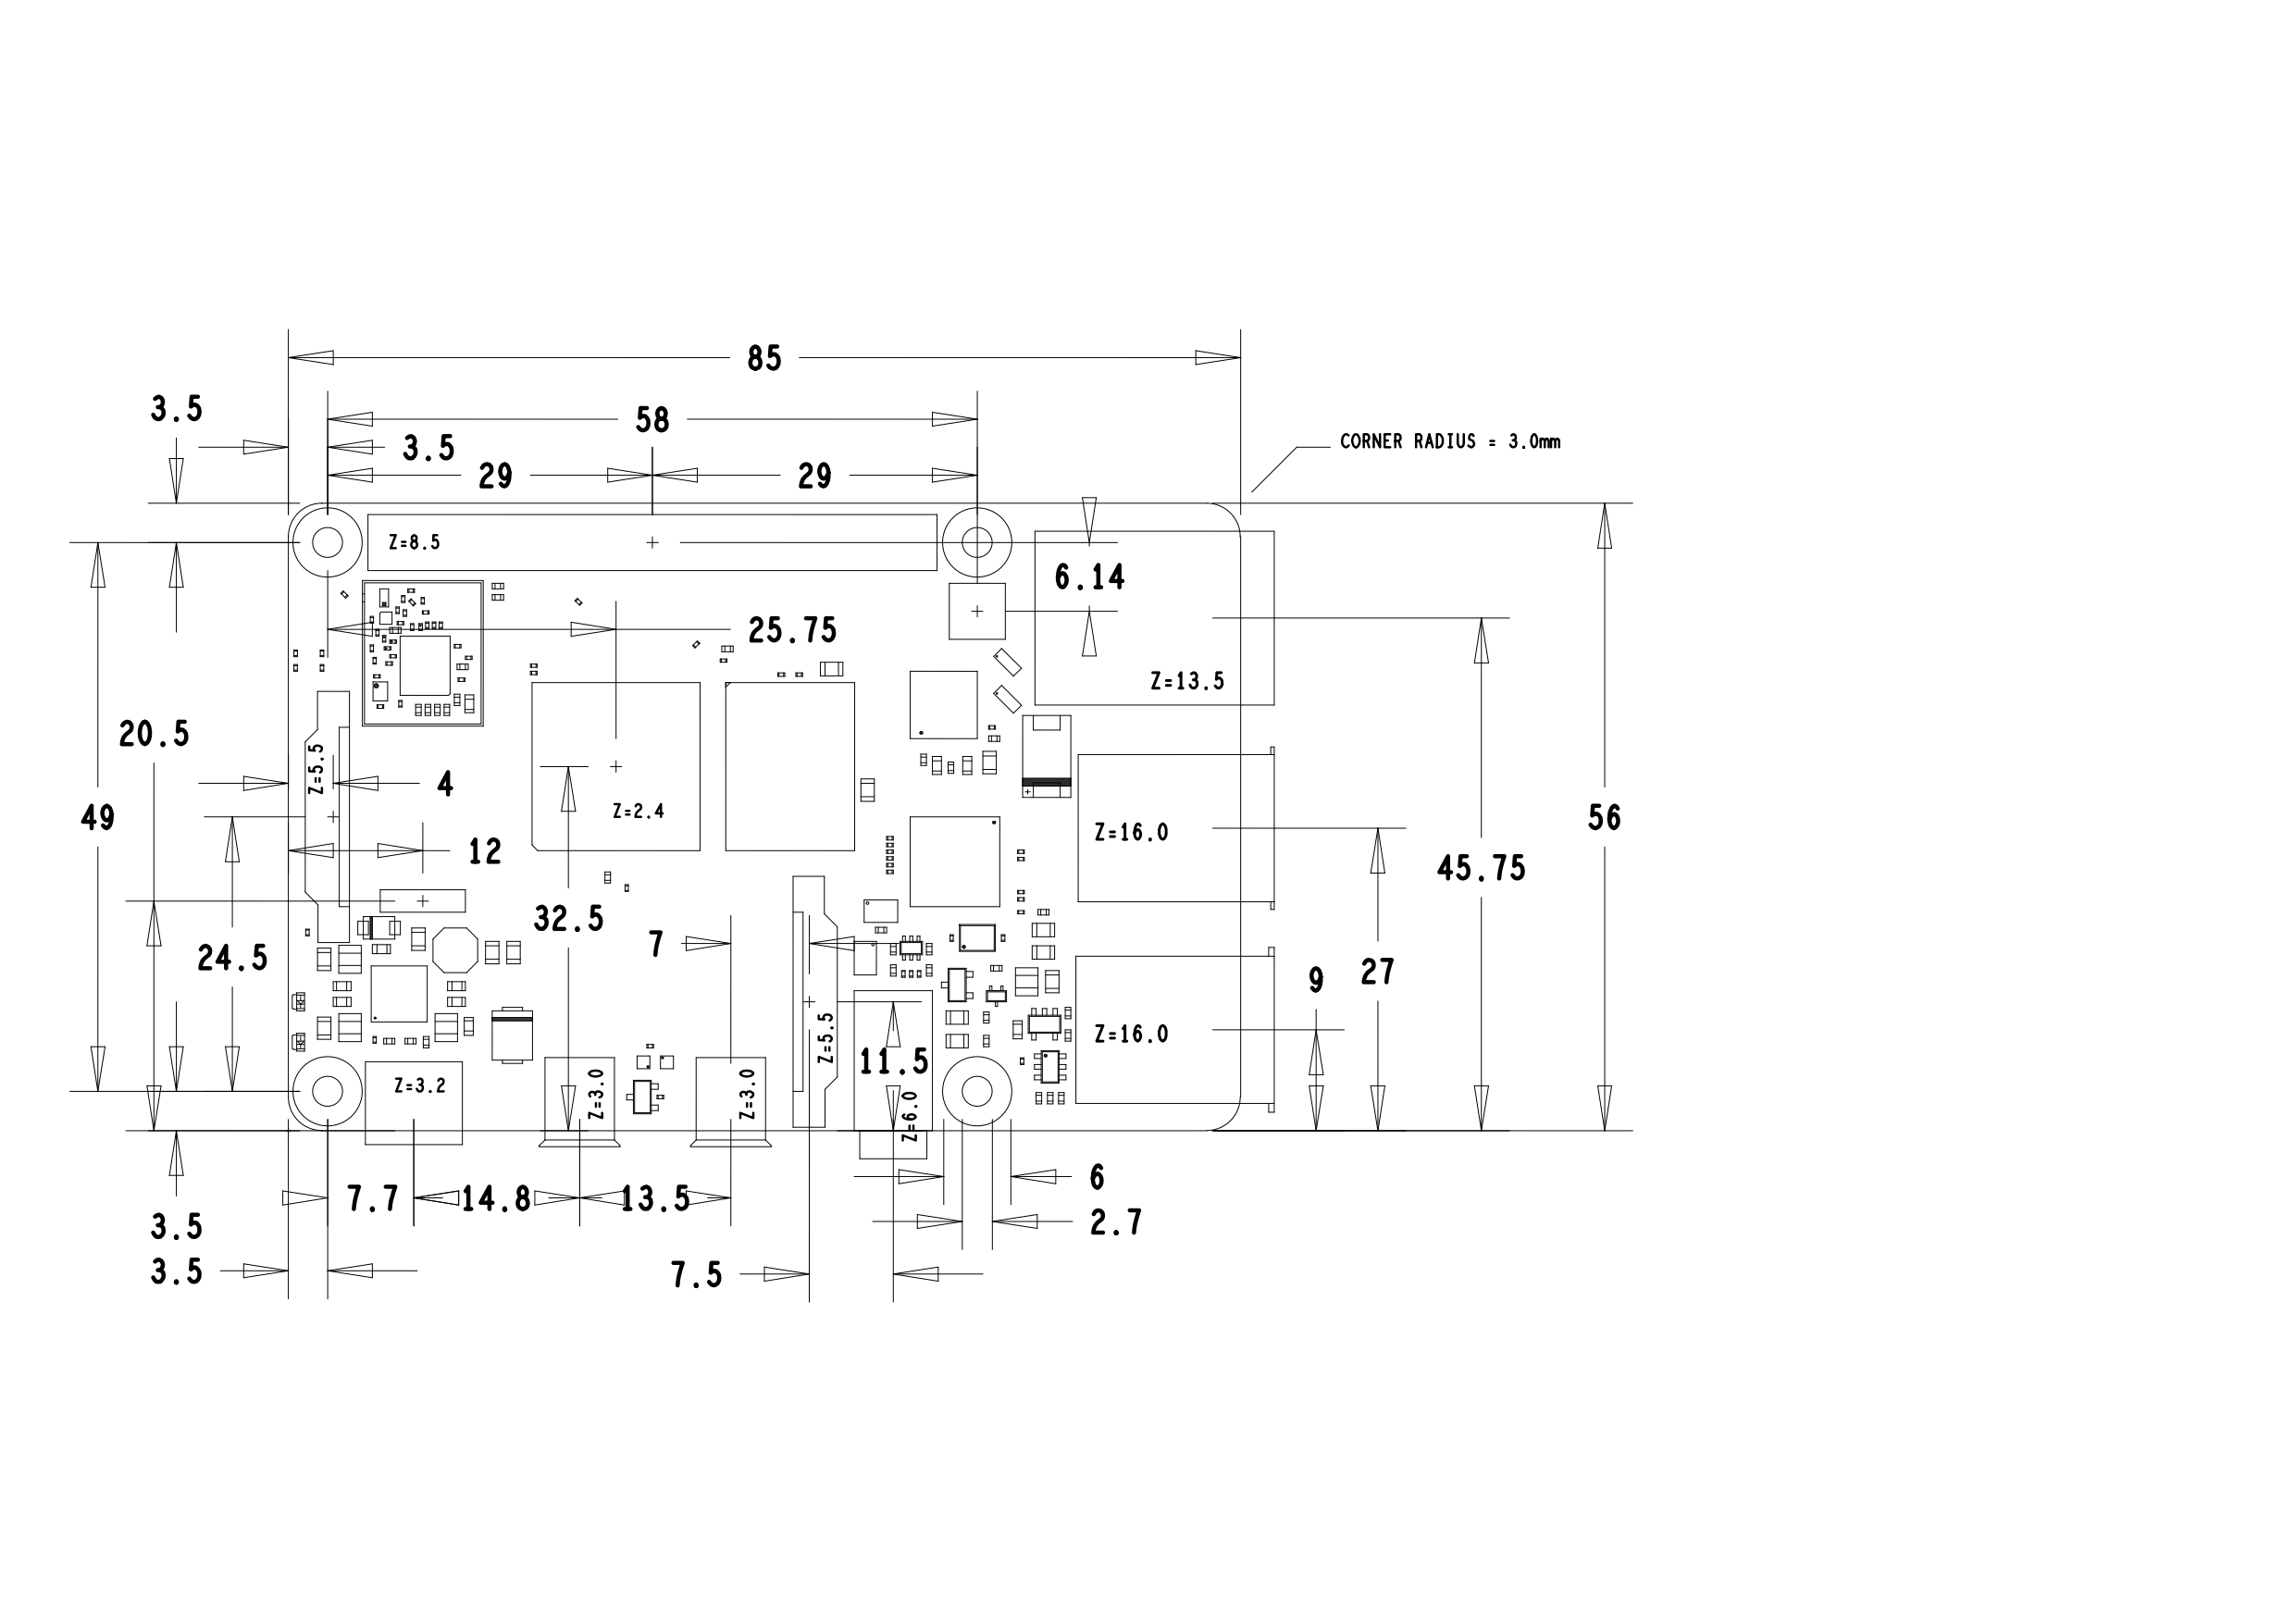
\includegraphics[width=\linewidth, angle=90]{texs/appendix/data/techspecs/pimechdraw.jpg}
    \caption{Raspberry Pi 4 Model B Mechanical Drawing}
    \label{fig:rpi-2}
\end{figure}

\subsection{Raspberry Pi Camera Module V2}

\begin{figure}[H]
    \centering
    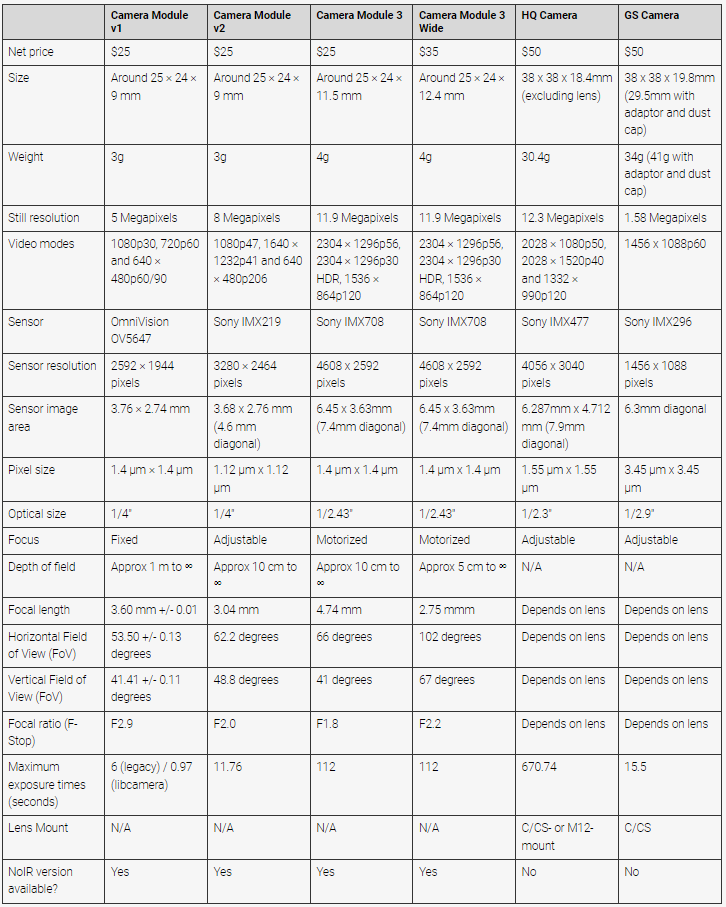
\includegraphics[width=0.85\linewidth]{texs/appendix/data/techspecs/cameraspecs.png}
    \caption{Raspberry Pi Camera Module V2 Technical Specifications}
    \label{fig:picam-1}
\end{figure}

\begin{figure}[H]
    \centering
    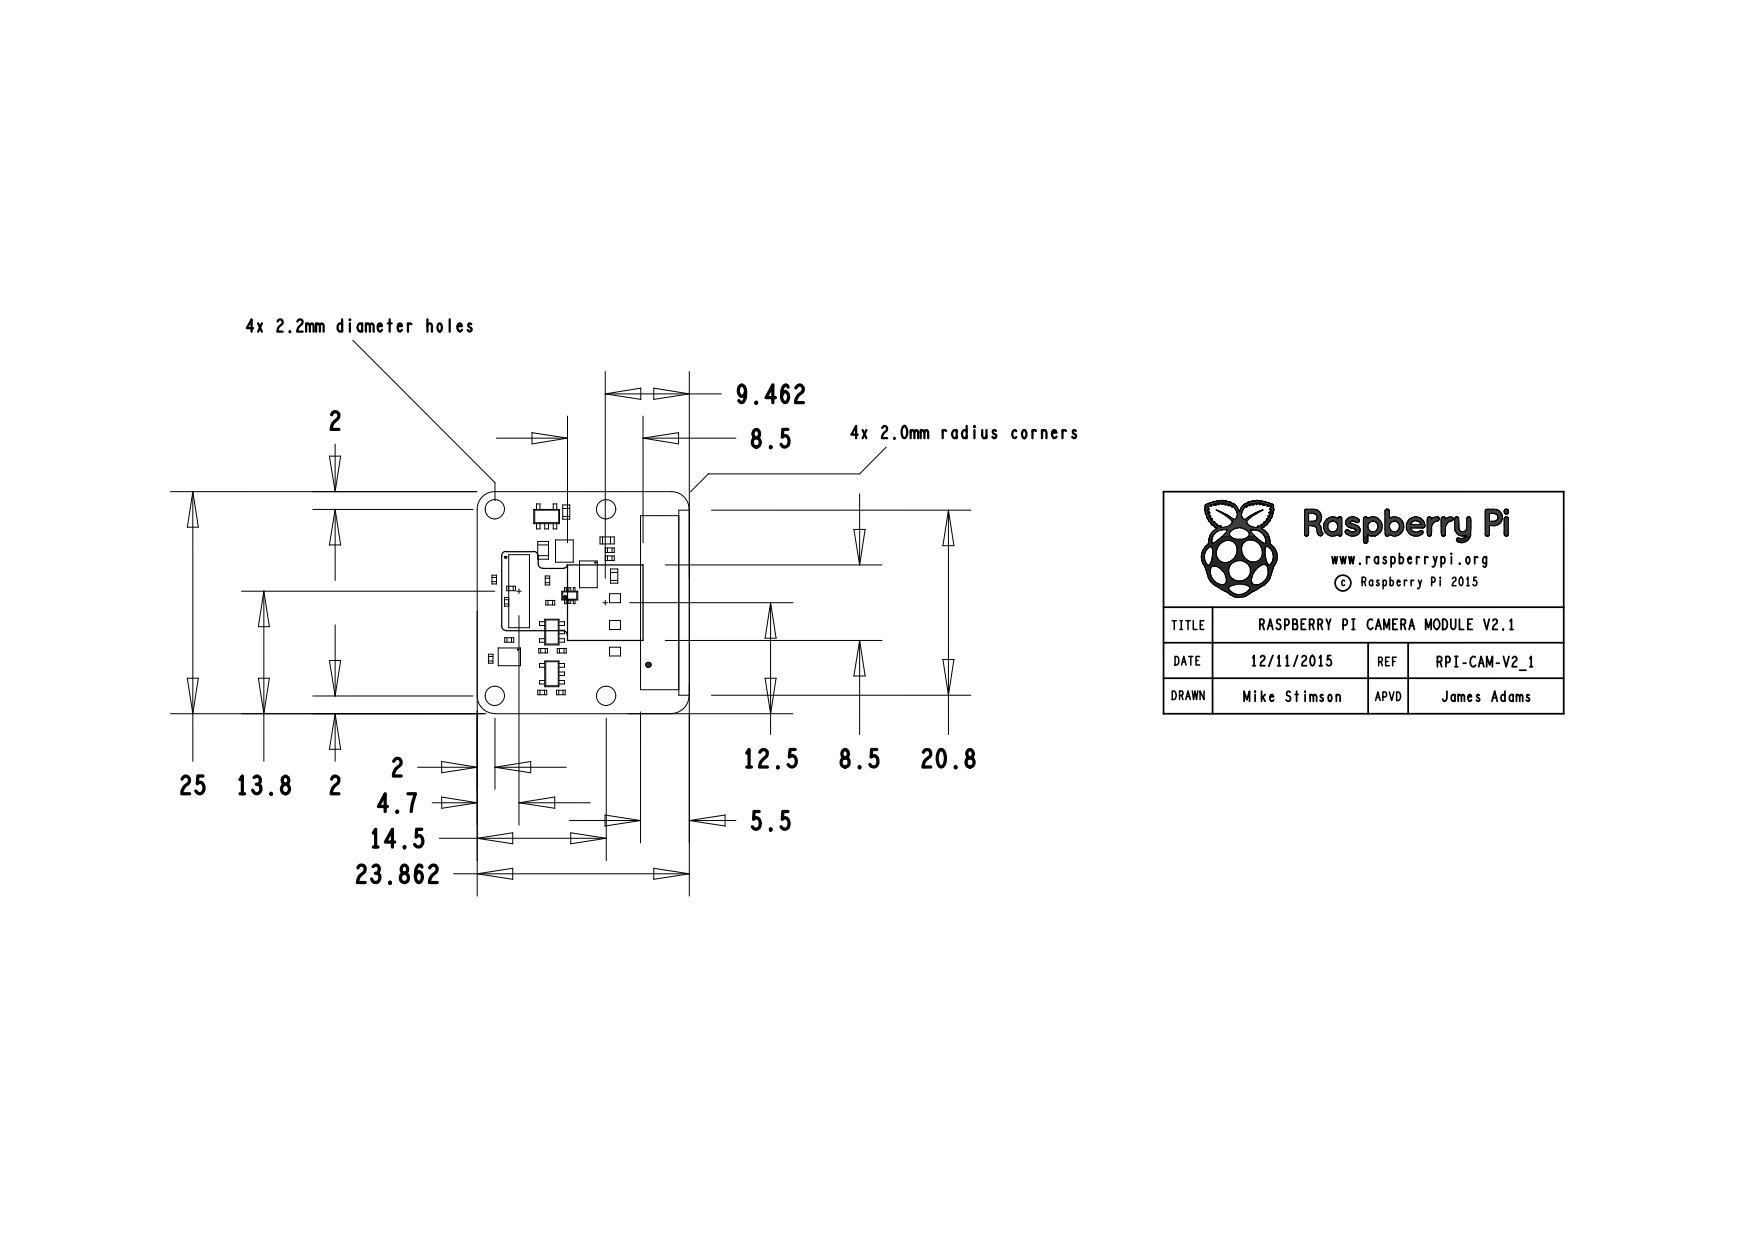
\includegraphics[width=\linewidth, angle=90]{texs/appendix/data/techspecs/cameramechdraw.jpg}
    \caption{Raspberry Pi Camera Module V2 Mechanical Drawing}
    \label{fig:picam-2}
\end{figure}

\subsection{Waveshare 7inch HDMI LCD (H)}

\begin{figure}[H]
    \centering
    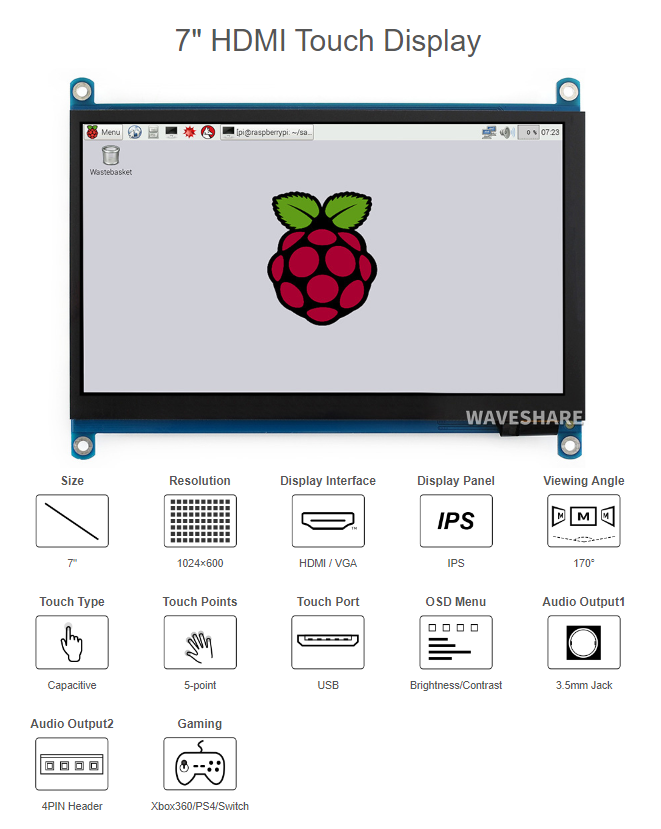
\includegraphics[width=0.85\linewidth]{texs/appendix/data/techspecs/screen1.png}
    \caption{Waveshare 7inch HDMI LCD (H) Technical Specifications -1 }
    \label{fig:lcd-1}
\end{figure}

\begin{figure}[H]
    \centering
    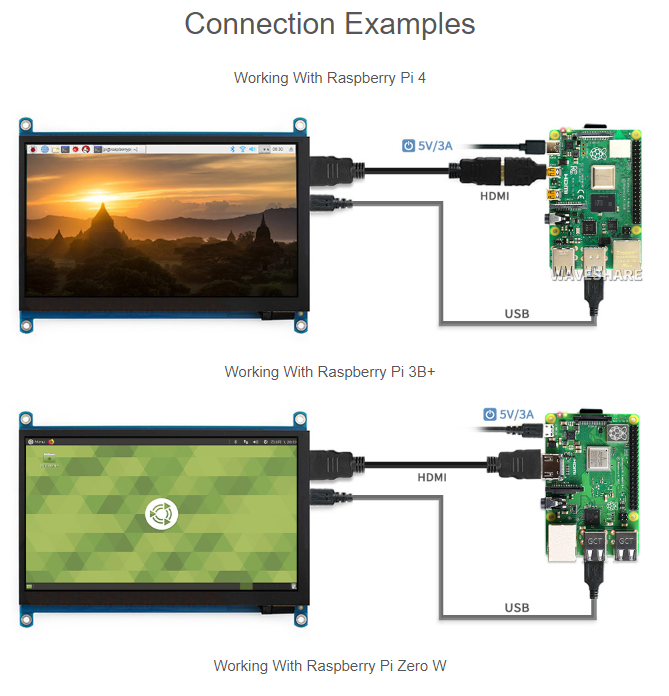
\includegraphics[width=0.85\linewidth]{texs/appendix/data/techspecs/screen2.png}
    \caption{Waveshare 7inch HDMI LCD (H) Technical Specifications -2 }
    \label{fig:lcd-2}
\end{figure}

\begin{figure}[H]
    \centering
    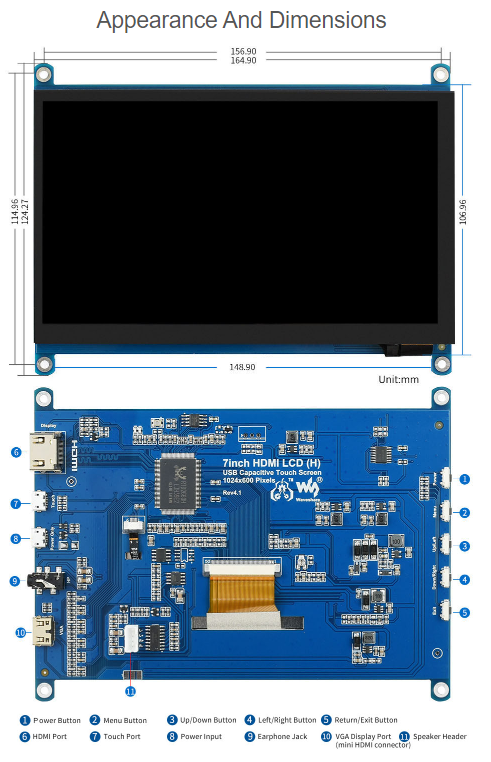
\includegraphics[width=0.85\linewidth]{texs/appendix/data/techspecs/screen3.png}
    \caption{Waveshare 7inch HDMI LCD (H) Technical Specifications -3 }
    \label{fig:lcd-3}
\end{figure}

\subsection{Veektomx VT103}

\begin{figure}[H]
    \centering
    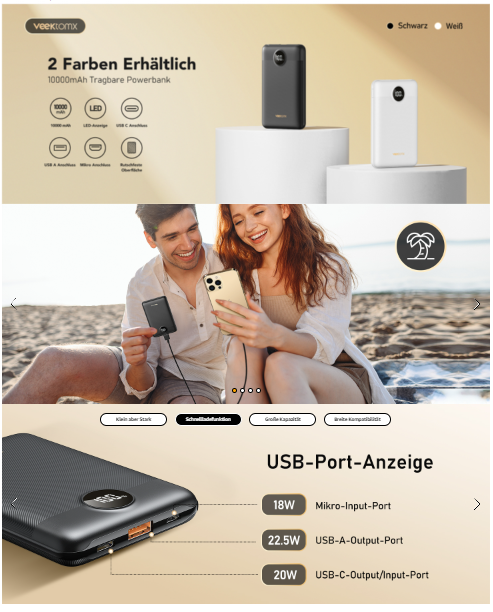
\includegraphics[width=0.85\linewidth]{texs/appendix/data/techspecs/battspecs.png}
    \caption{Veektomx VT103 Technical Specifications }
    \label{fig:battery-1}
\end{figure}

\begin{figure}[H]
    \centering
    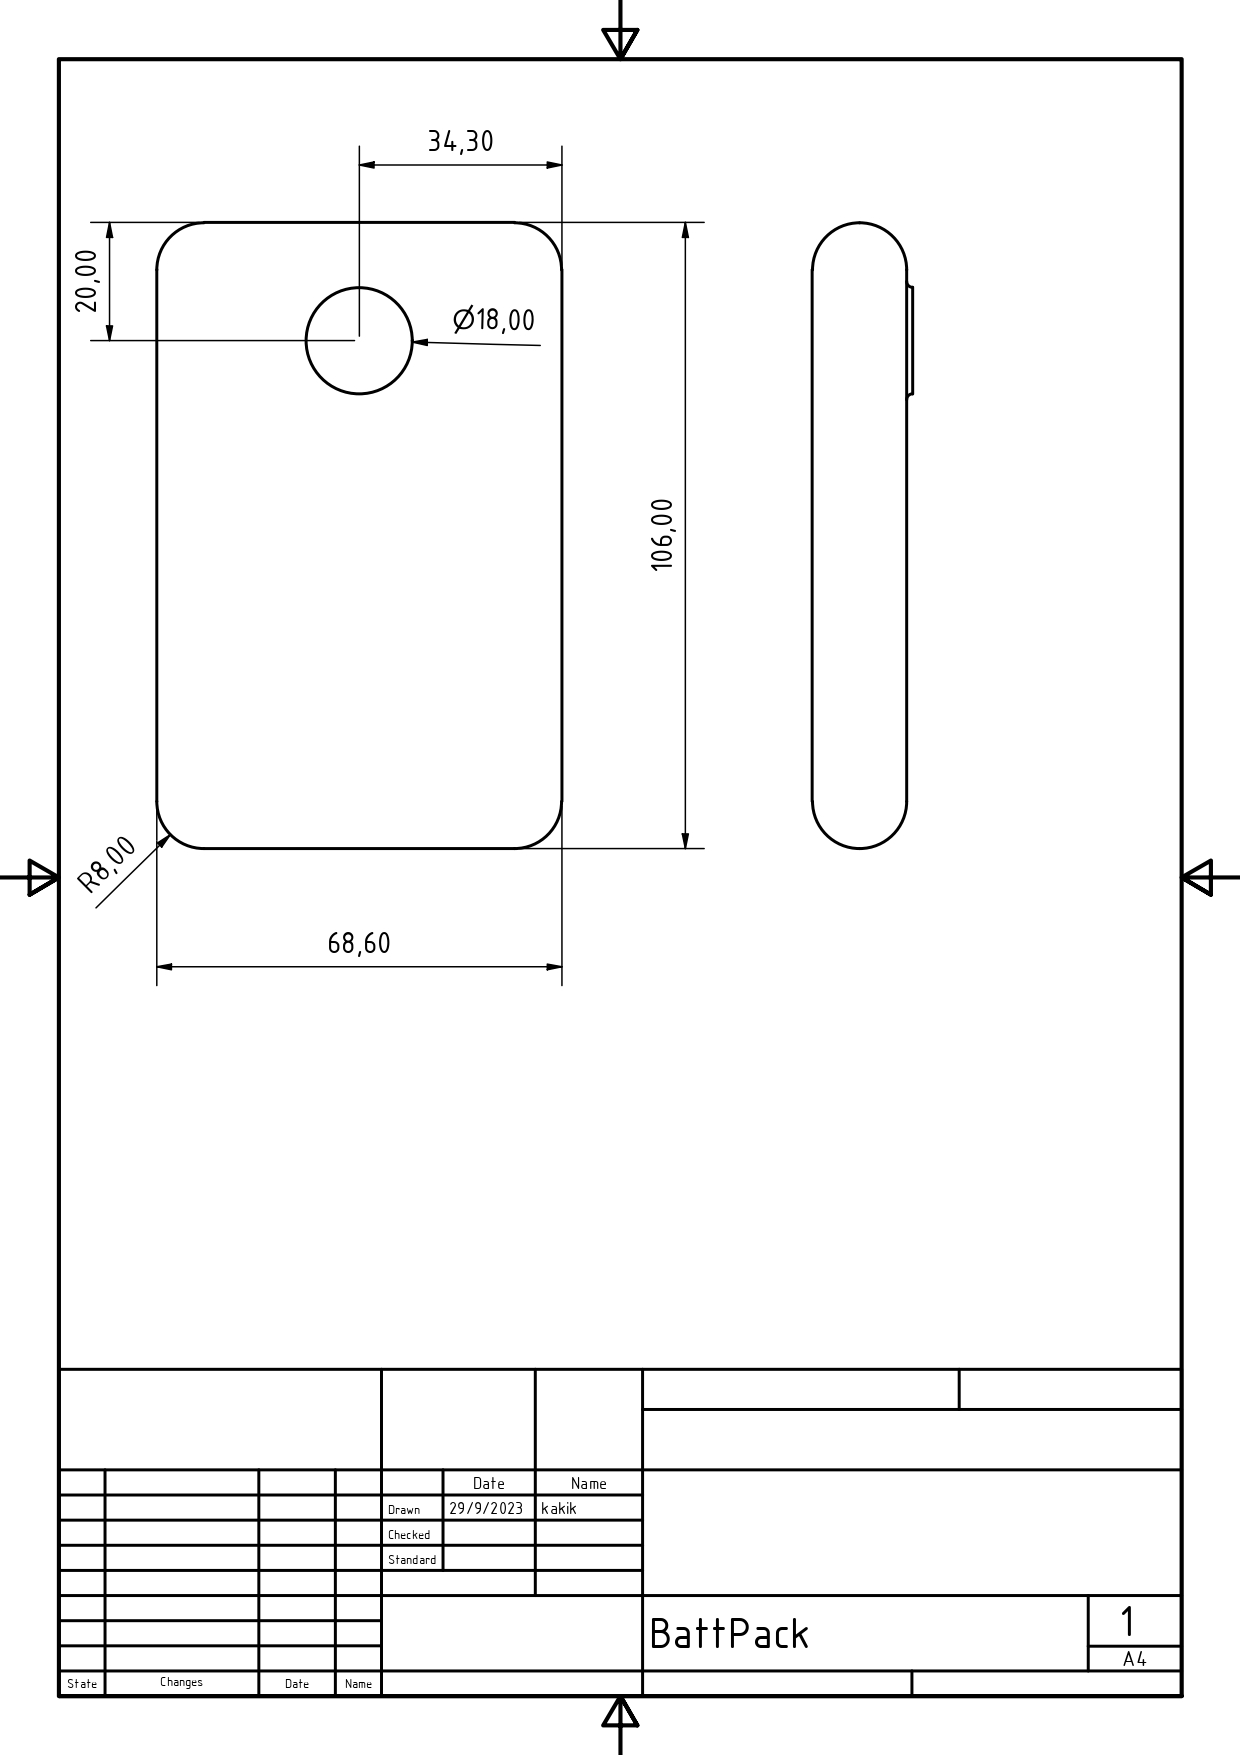
\includegraphics[width=0.85\linewidth]{texs/appendix/data/techspecs/battmechdraw.jpg}
    \caption{Veektomx VT103 Mechanical Drawing }
    \label{fig:battery-2}
\end{figure}

\subsection{Ruthex Brass Inserts}

\begin{figure}[H]
    \centering
    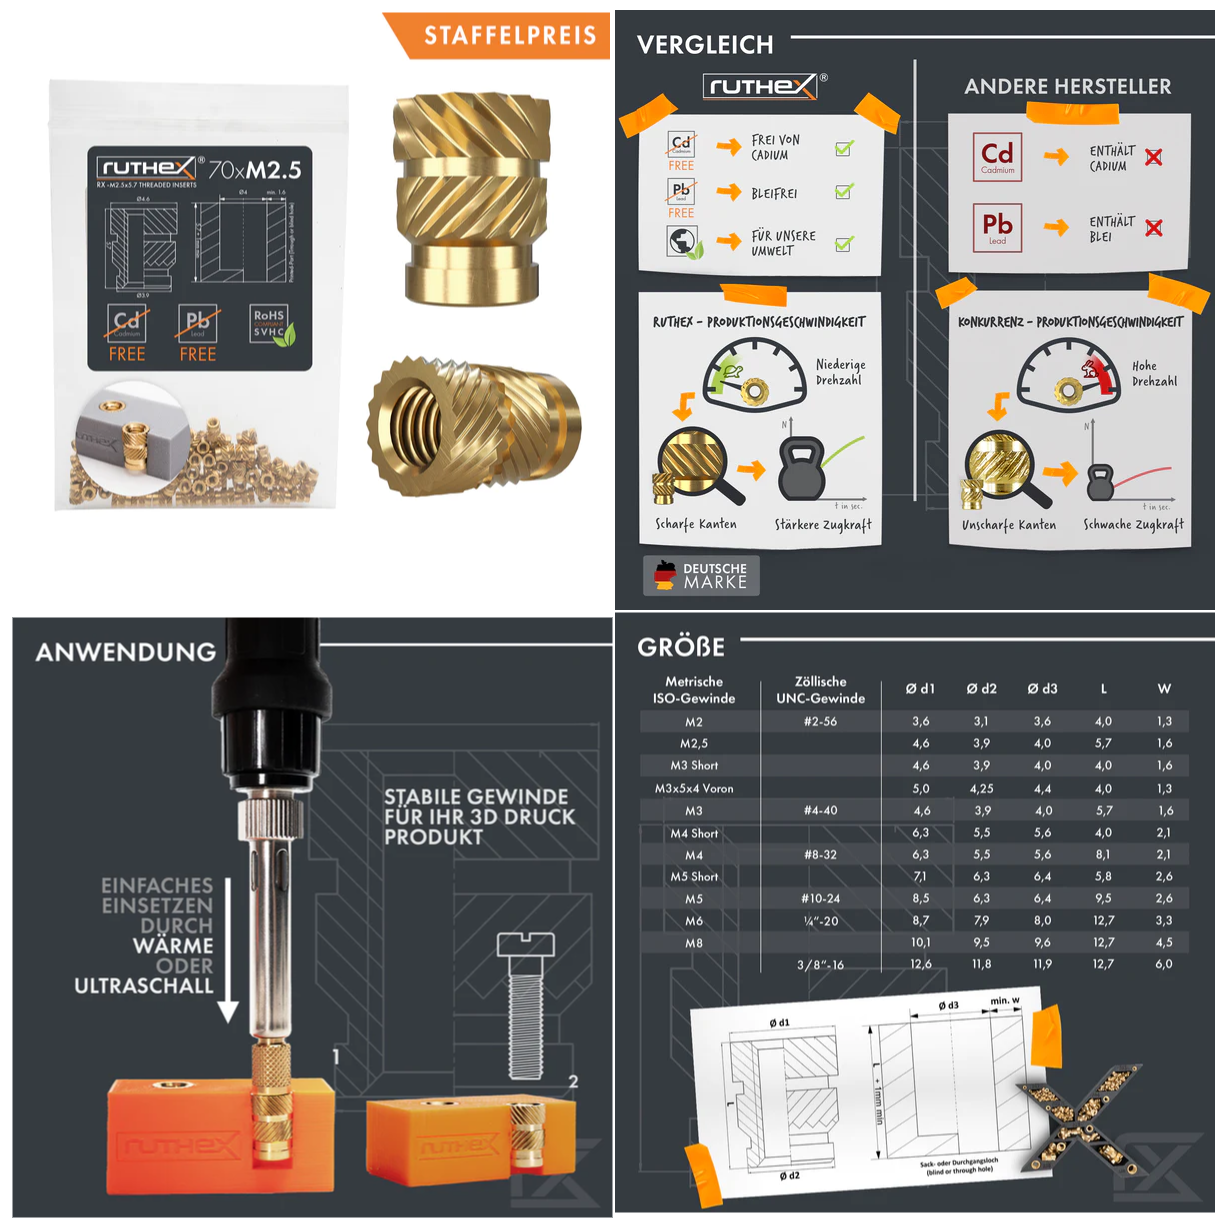
\includegraphics[width=0.85\linewidth]{texs/appendix/data/techspecs/ruthex.png}
    \caption{Ruthex Brass Inserts}
    \label{fig:insert-1}
\end{figure}

\section{Cost Calculation}
\label{appendix:cost-calculation}

\begin{figure}[H]
    \centering
    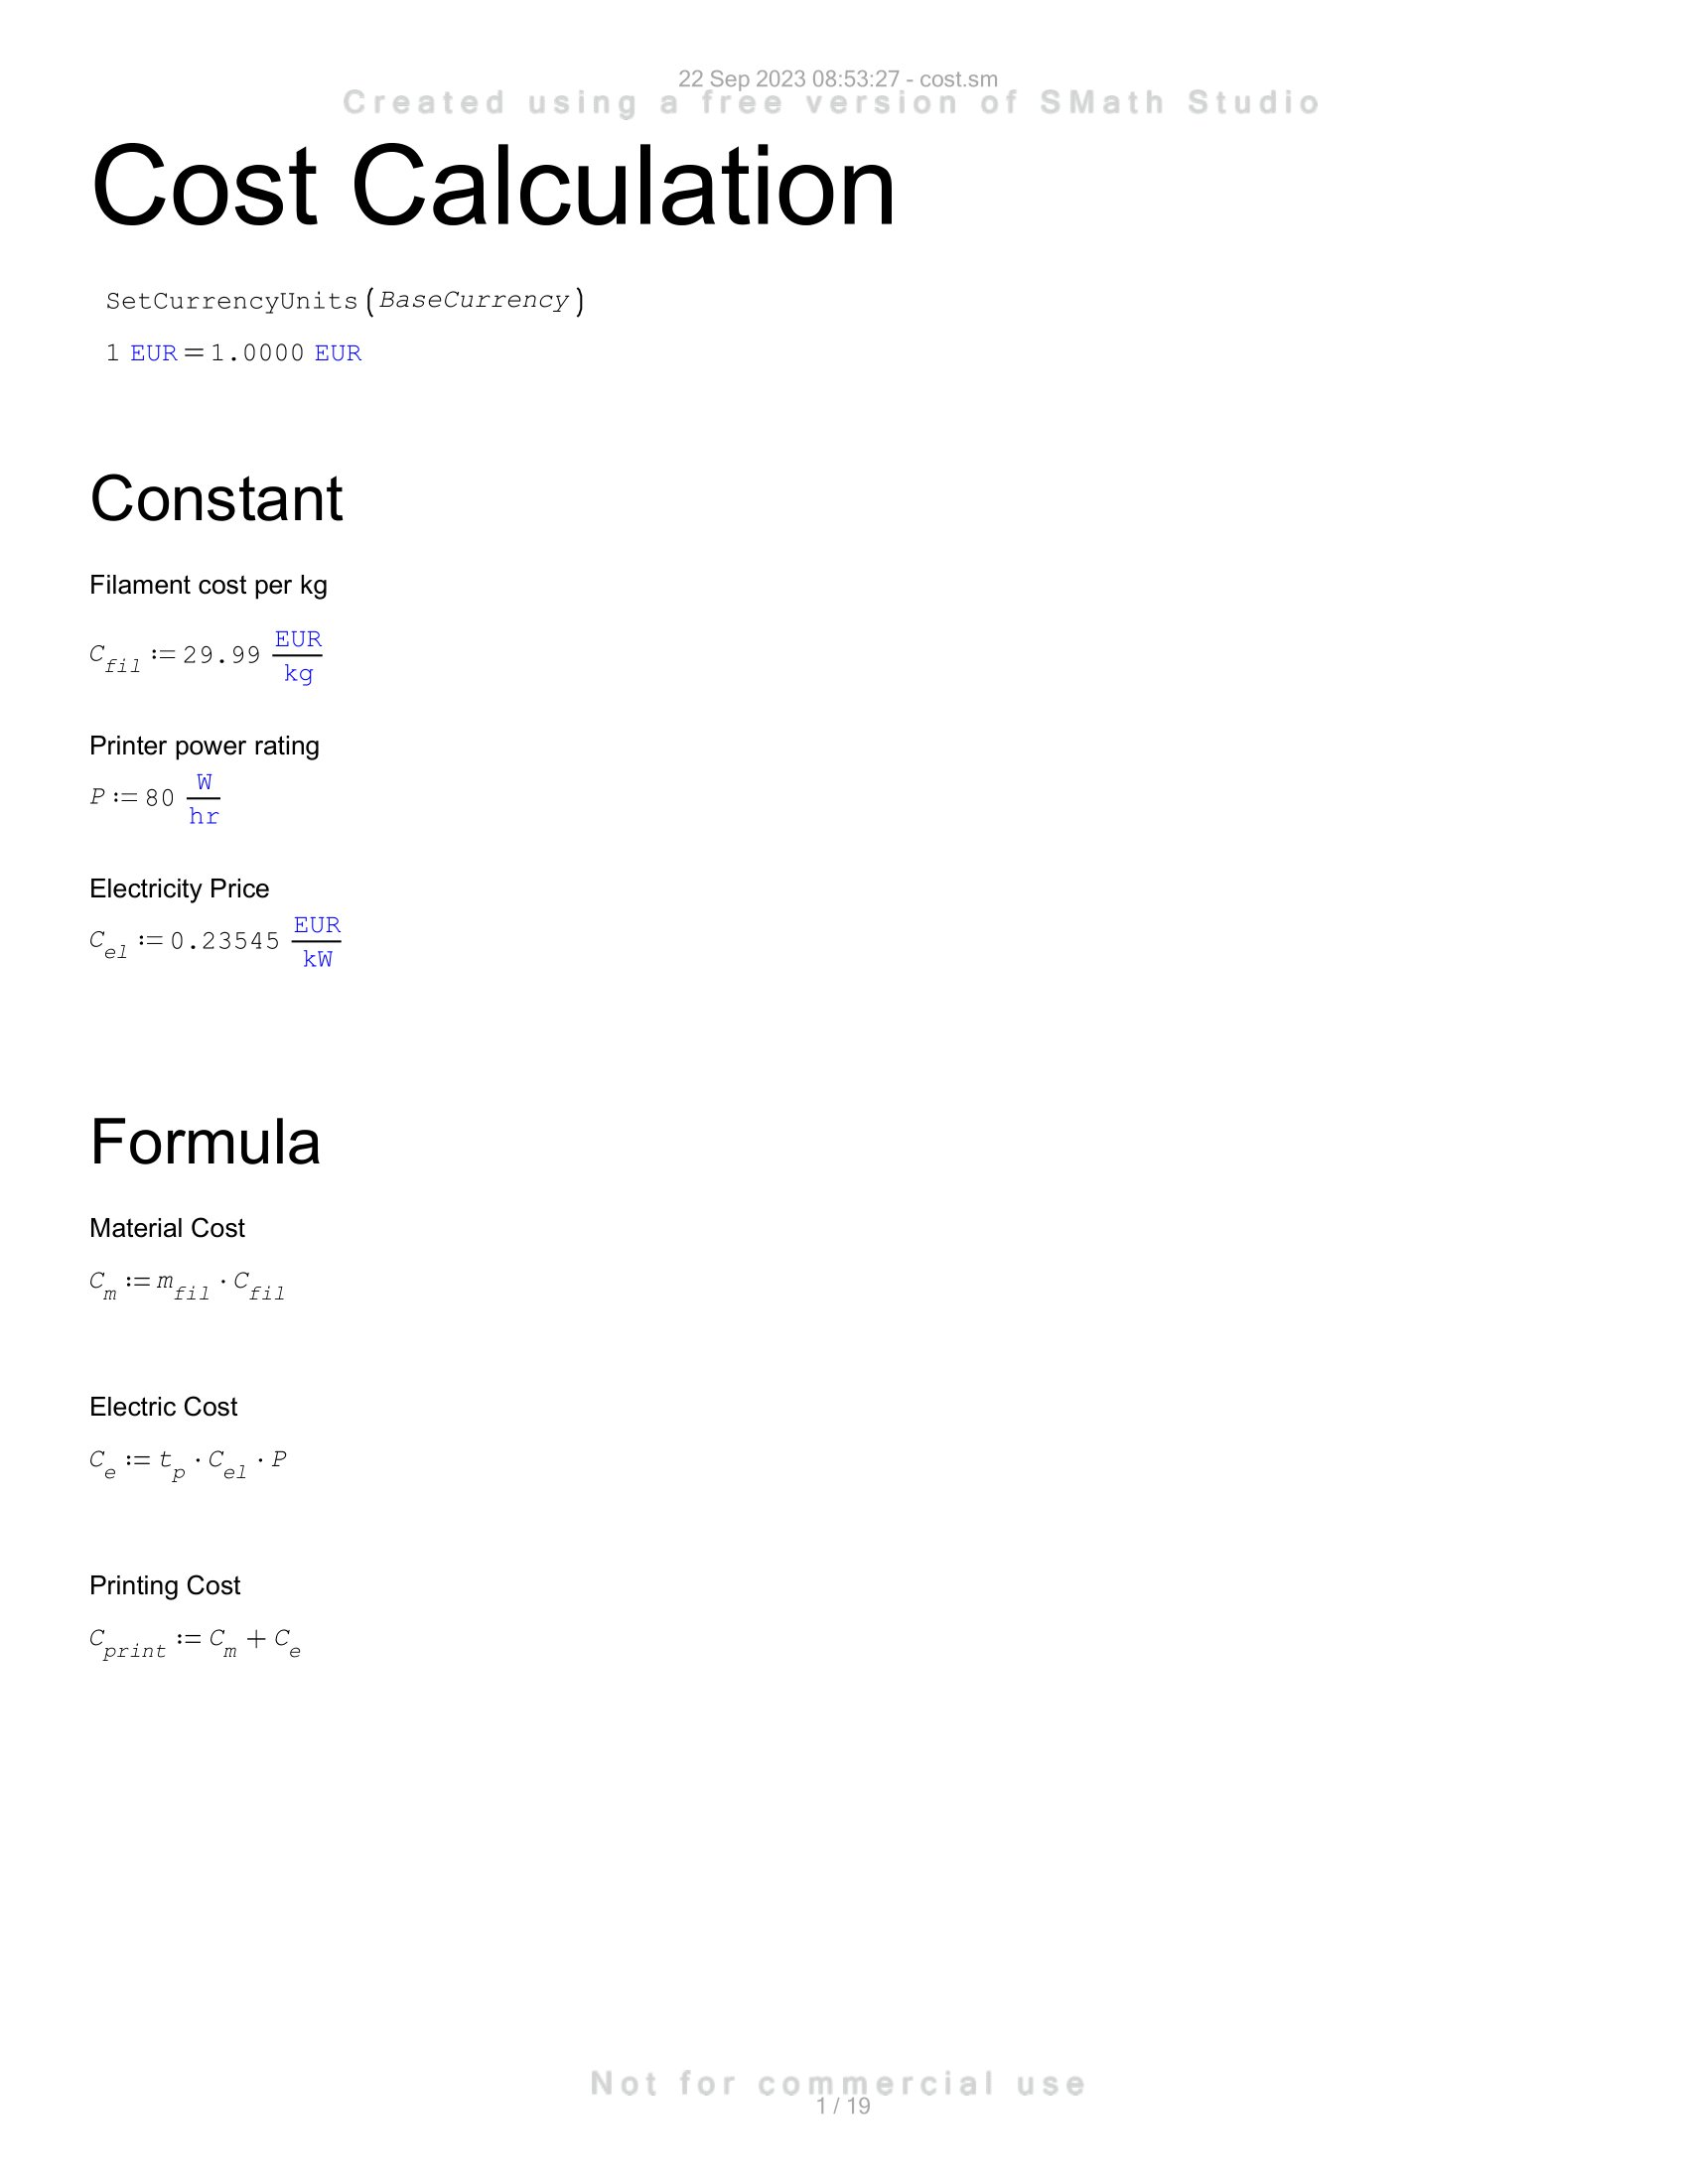
\includegraphics[width=\linewidth]{texs/appendix/data/costcalculation/cost1-01.jpg}
    \caption{Cost Calculation 1}
    \label{fig:cost-calculation-1}
\end{figure}

\begin{figure}[H]
    \centering
    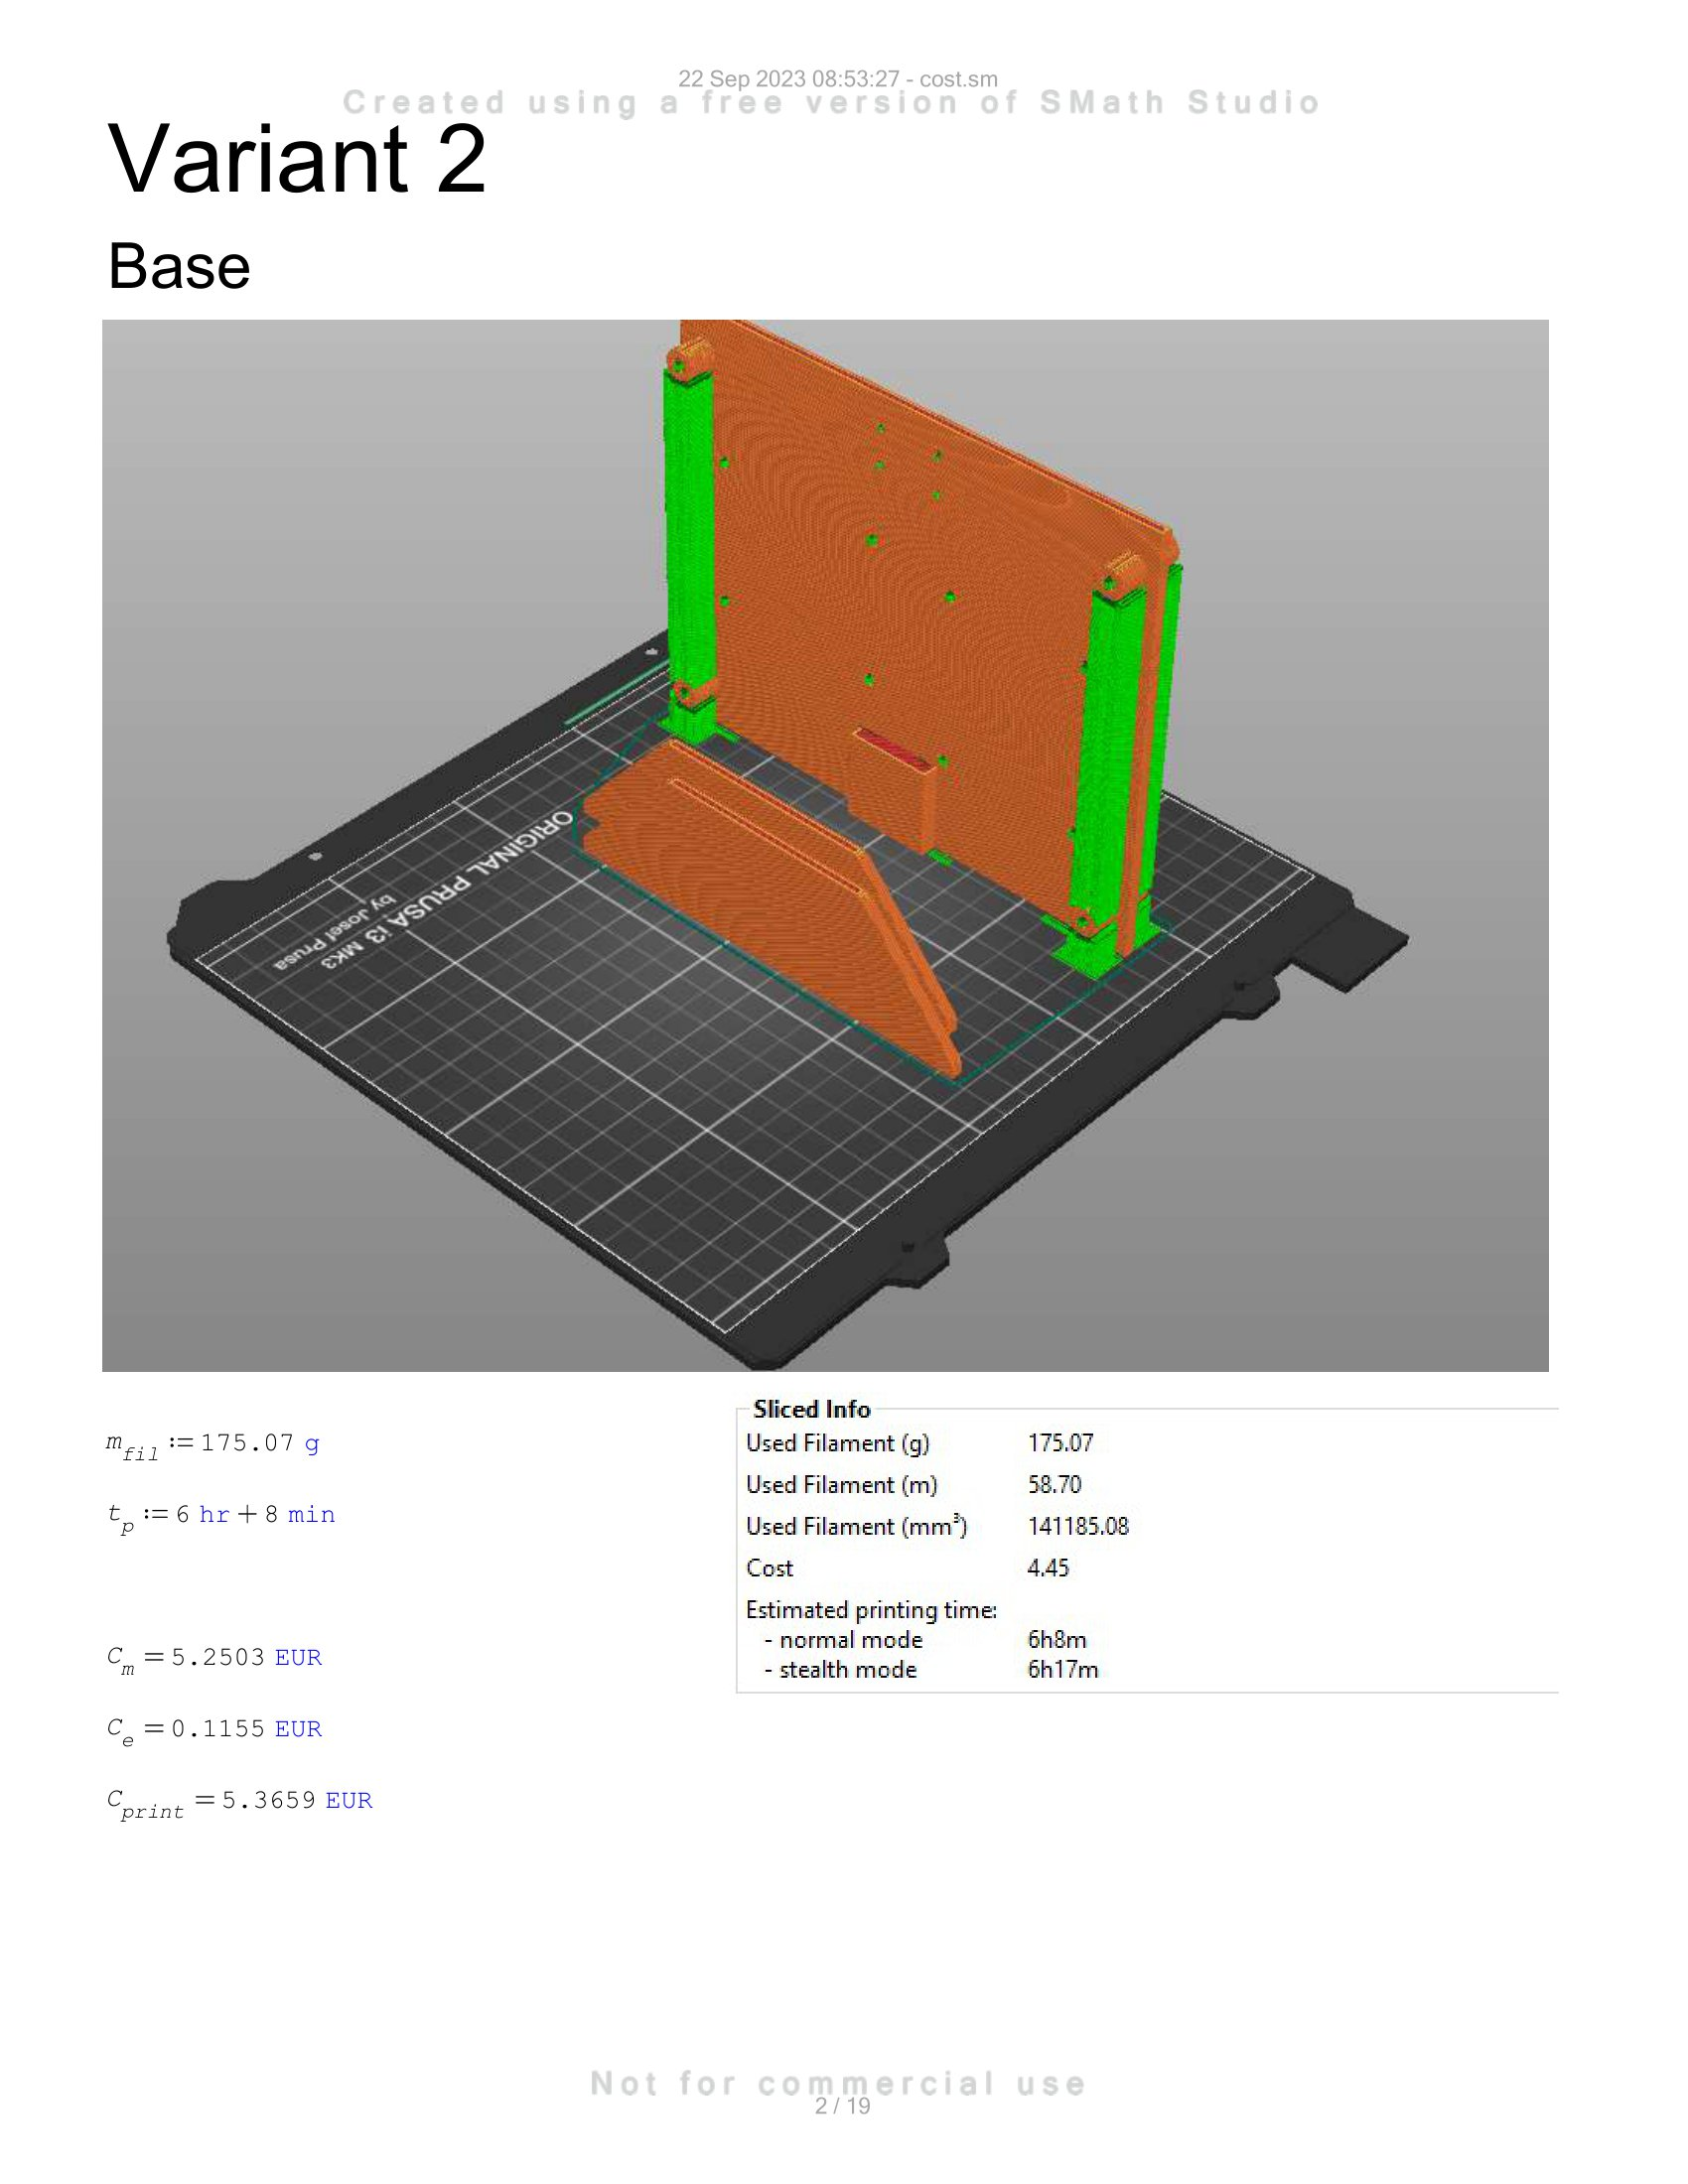
\includegraphics[width=\linewidth]{texs/appendix/data/costcalculation/cost1-02.jpg}
    \caption{Cost Calculation 2}
    \label{fig:cost-calculation-2}
\end{figure}

\begin{figure}[H]
    \centering
    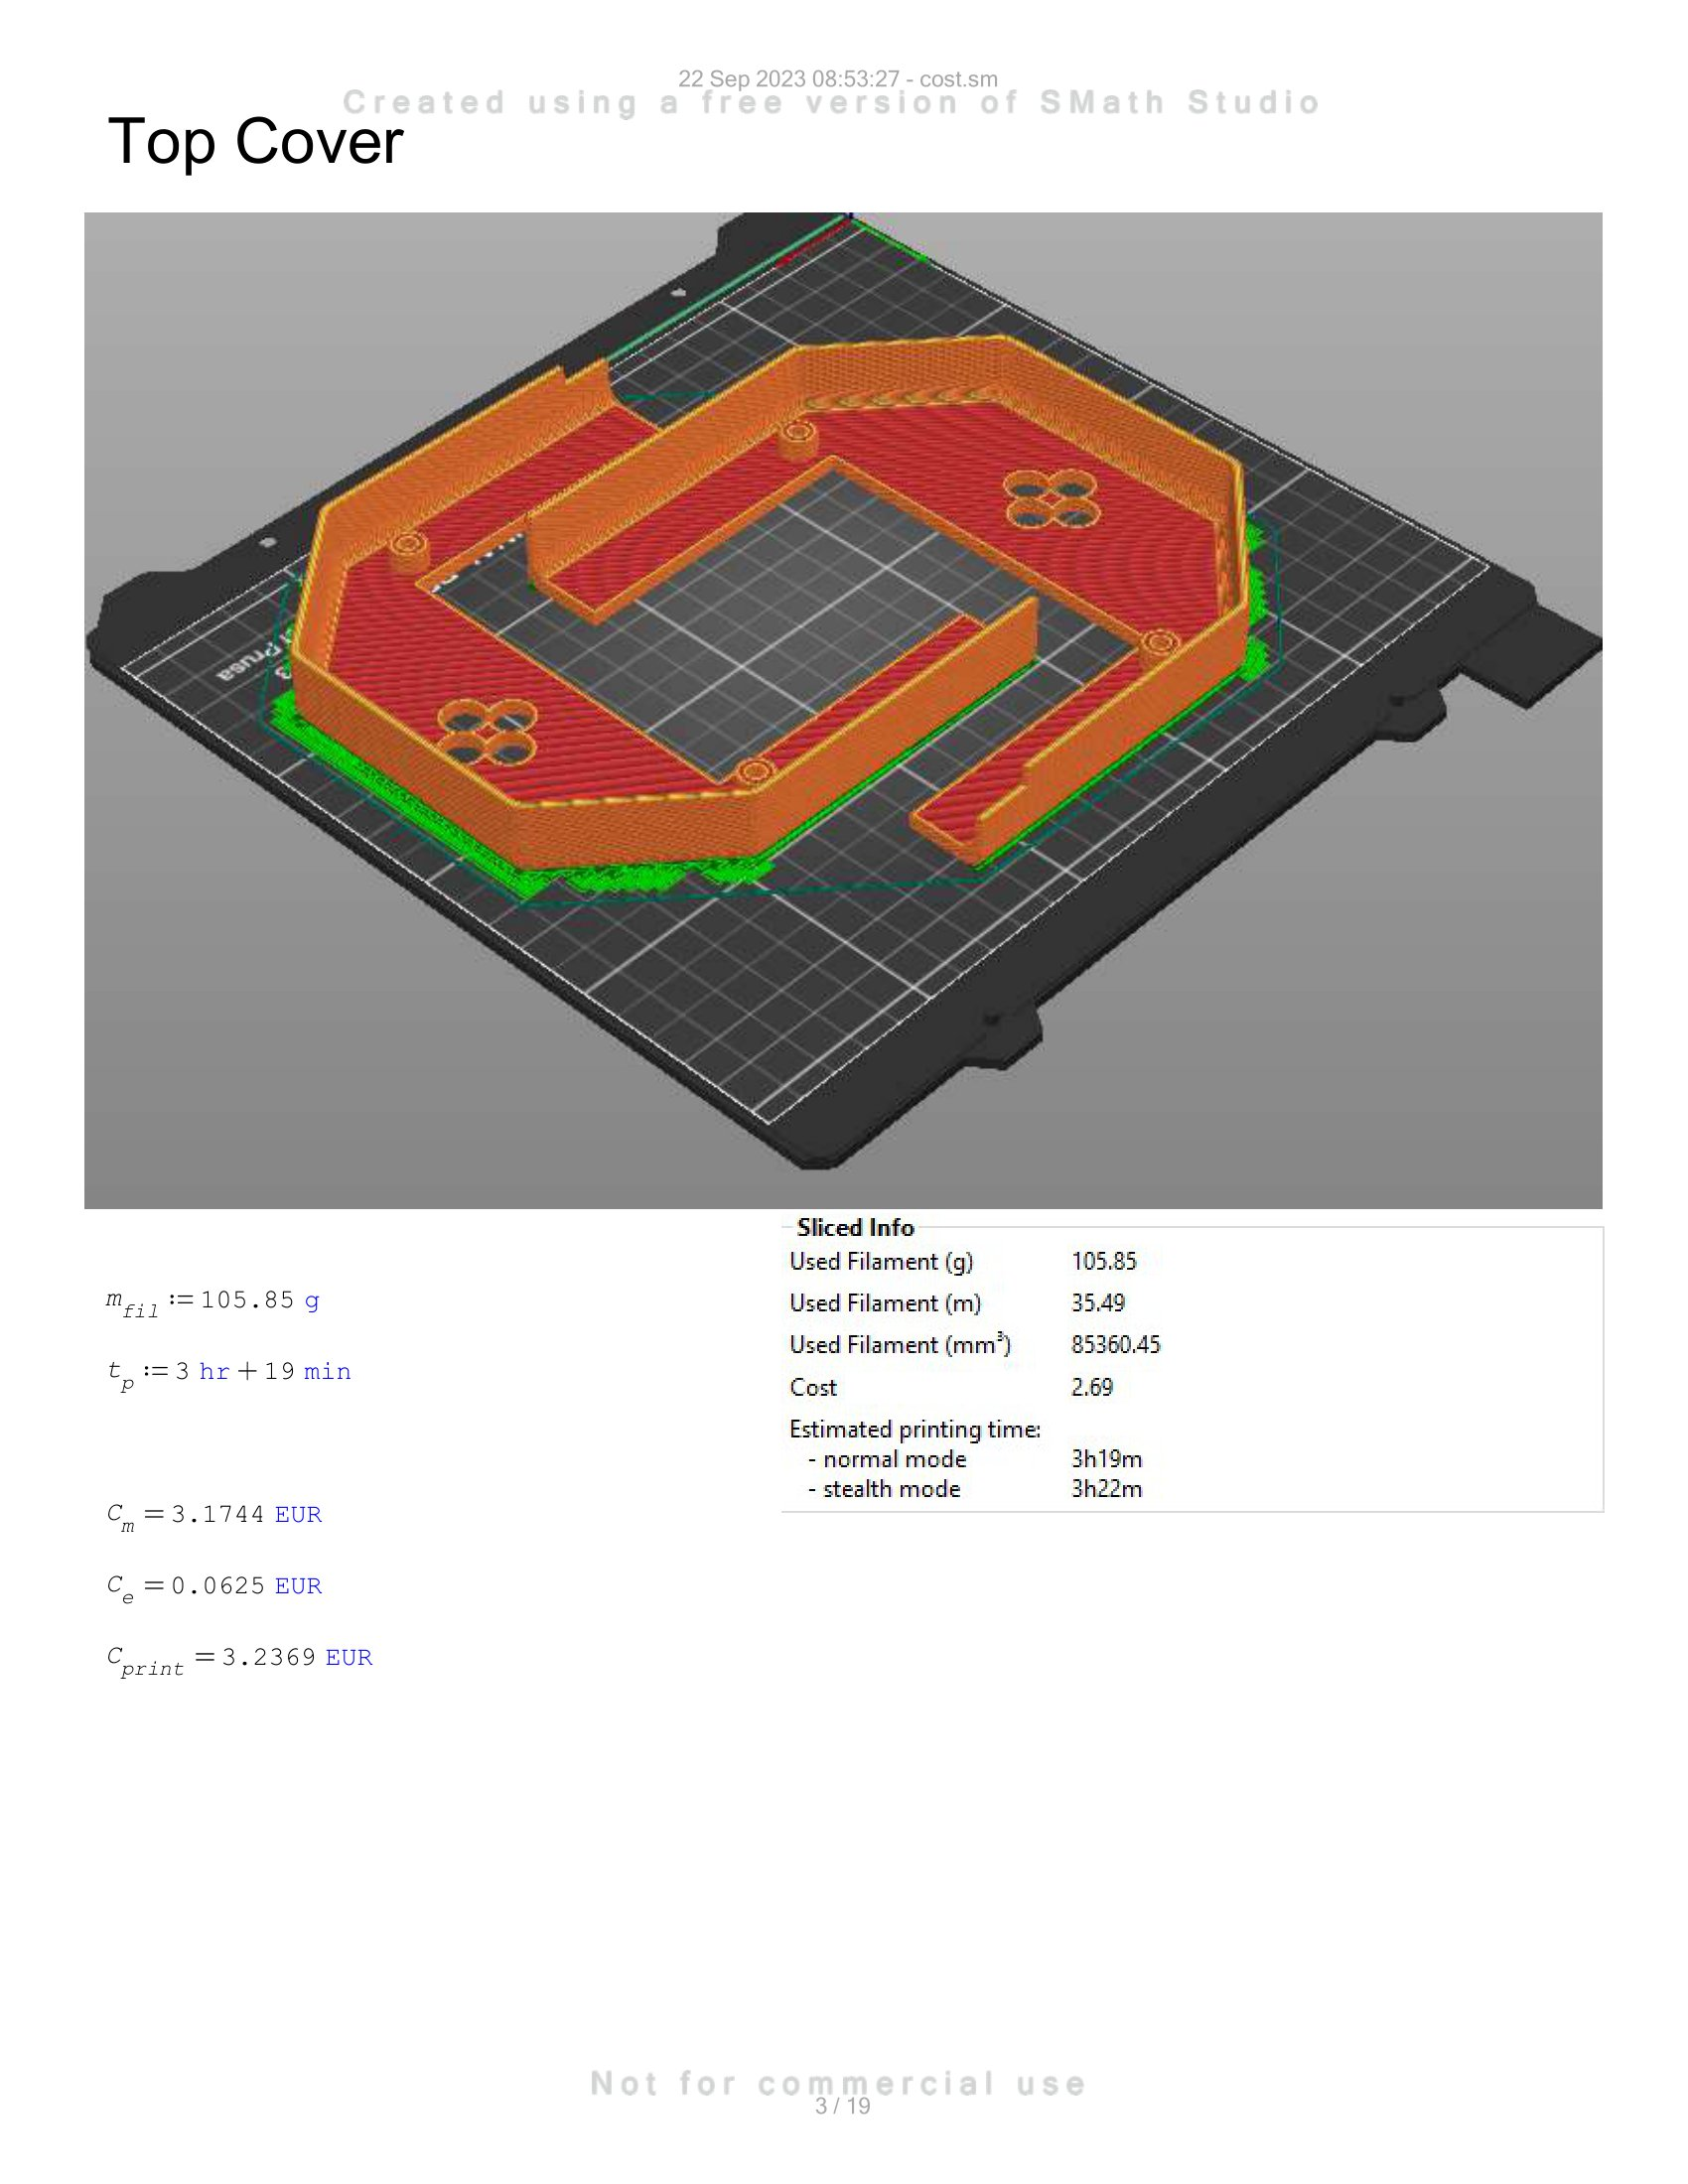
\includegraphics[width=\linewidth]{texs/appendix/data/costcalculation/cost1-03.jpg}
    \caption{Cost Calculation 3}
    \label{fig:cost-calculation-3}
\end{figure}

\begin{figure}[H]
    \centering
    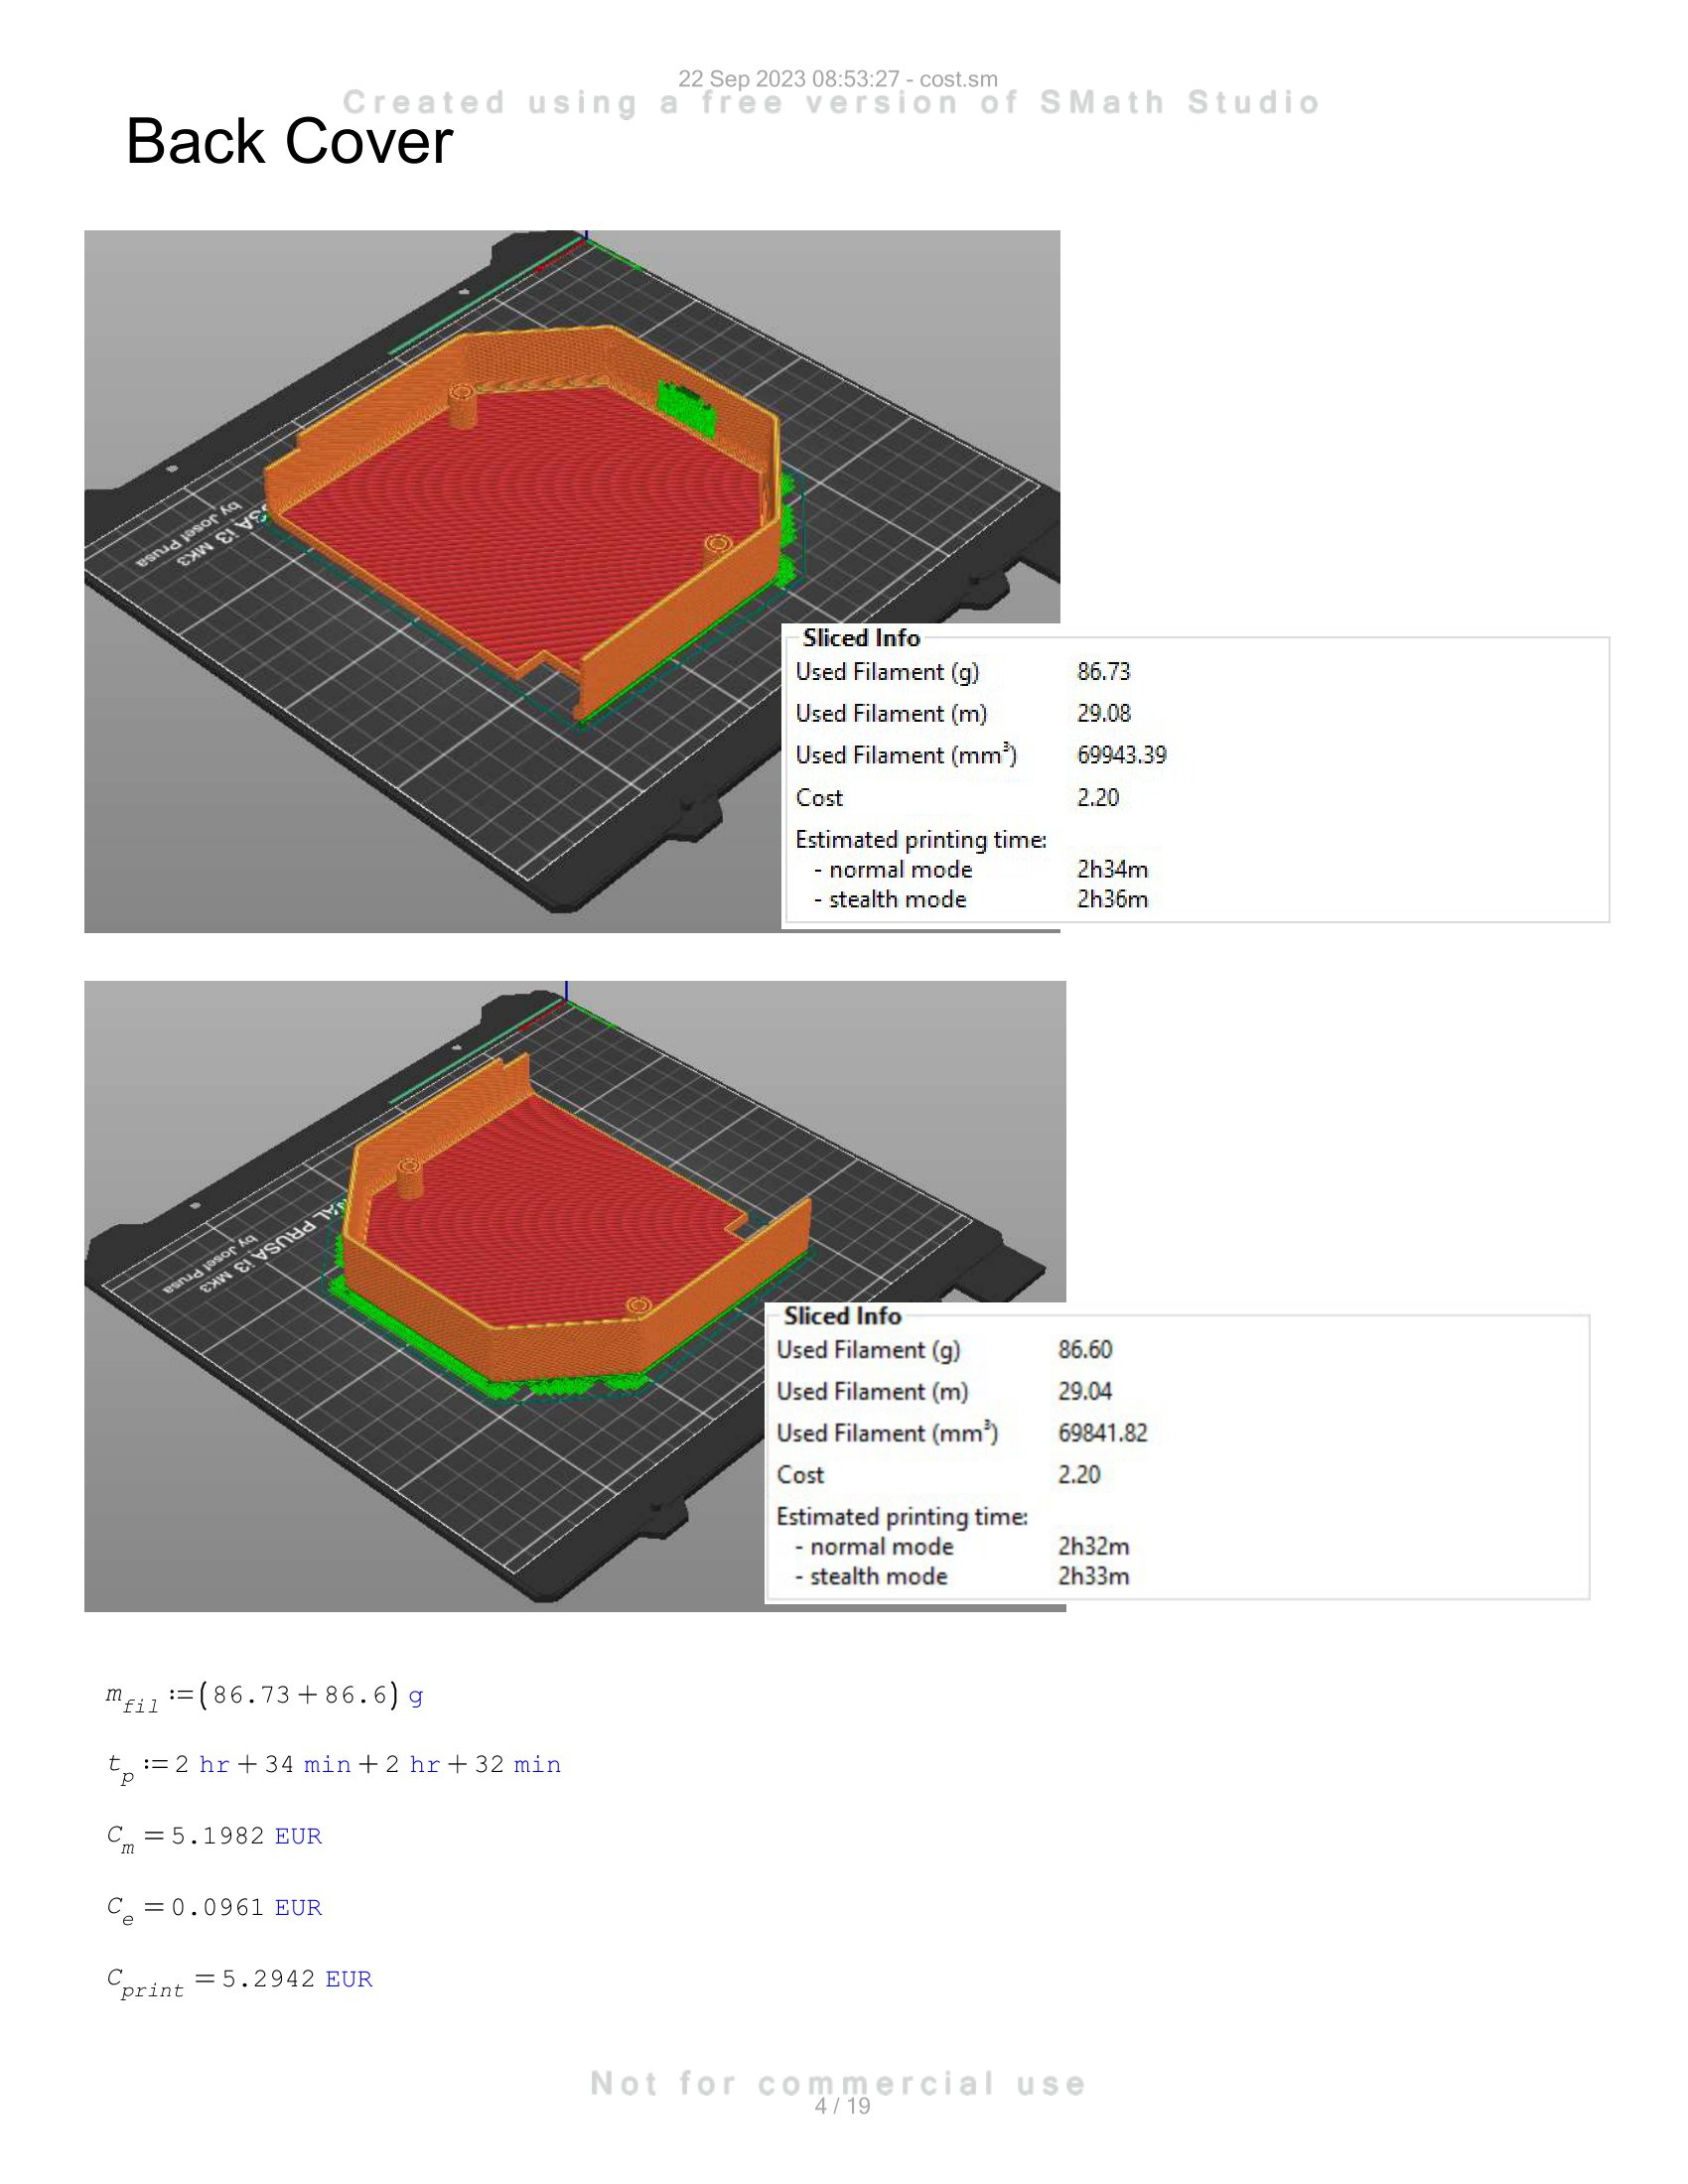
\includegraphics[width=\linewidth]{texs/appendix/data/costcalculation/cost1-04.jpg}
    \caption{Cost Calculation 4}
    \label{fig:cost-calculation-4}
\end{figure}

\begin{figure}[H]
    \centering
    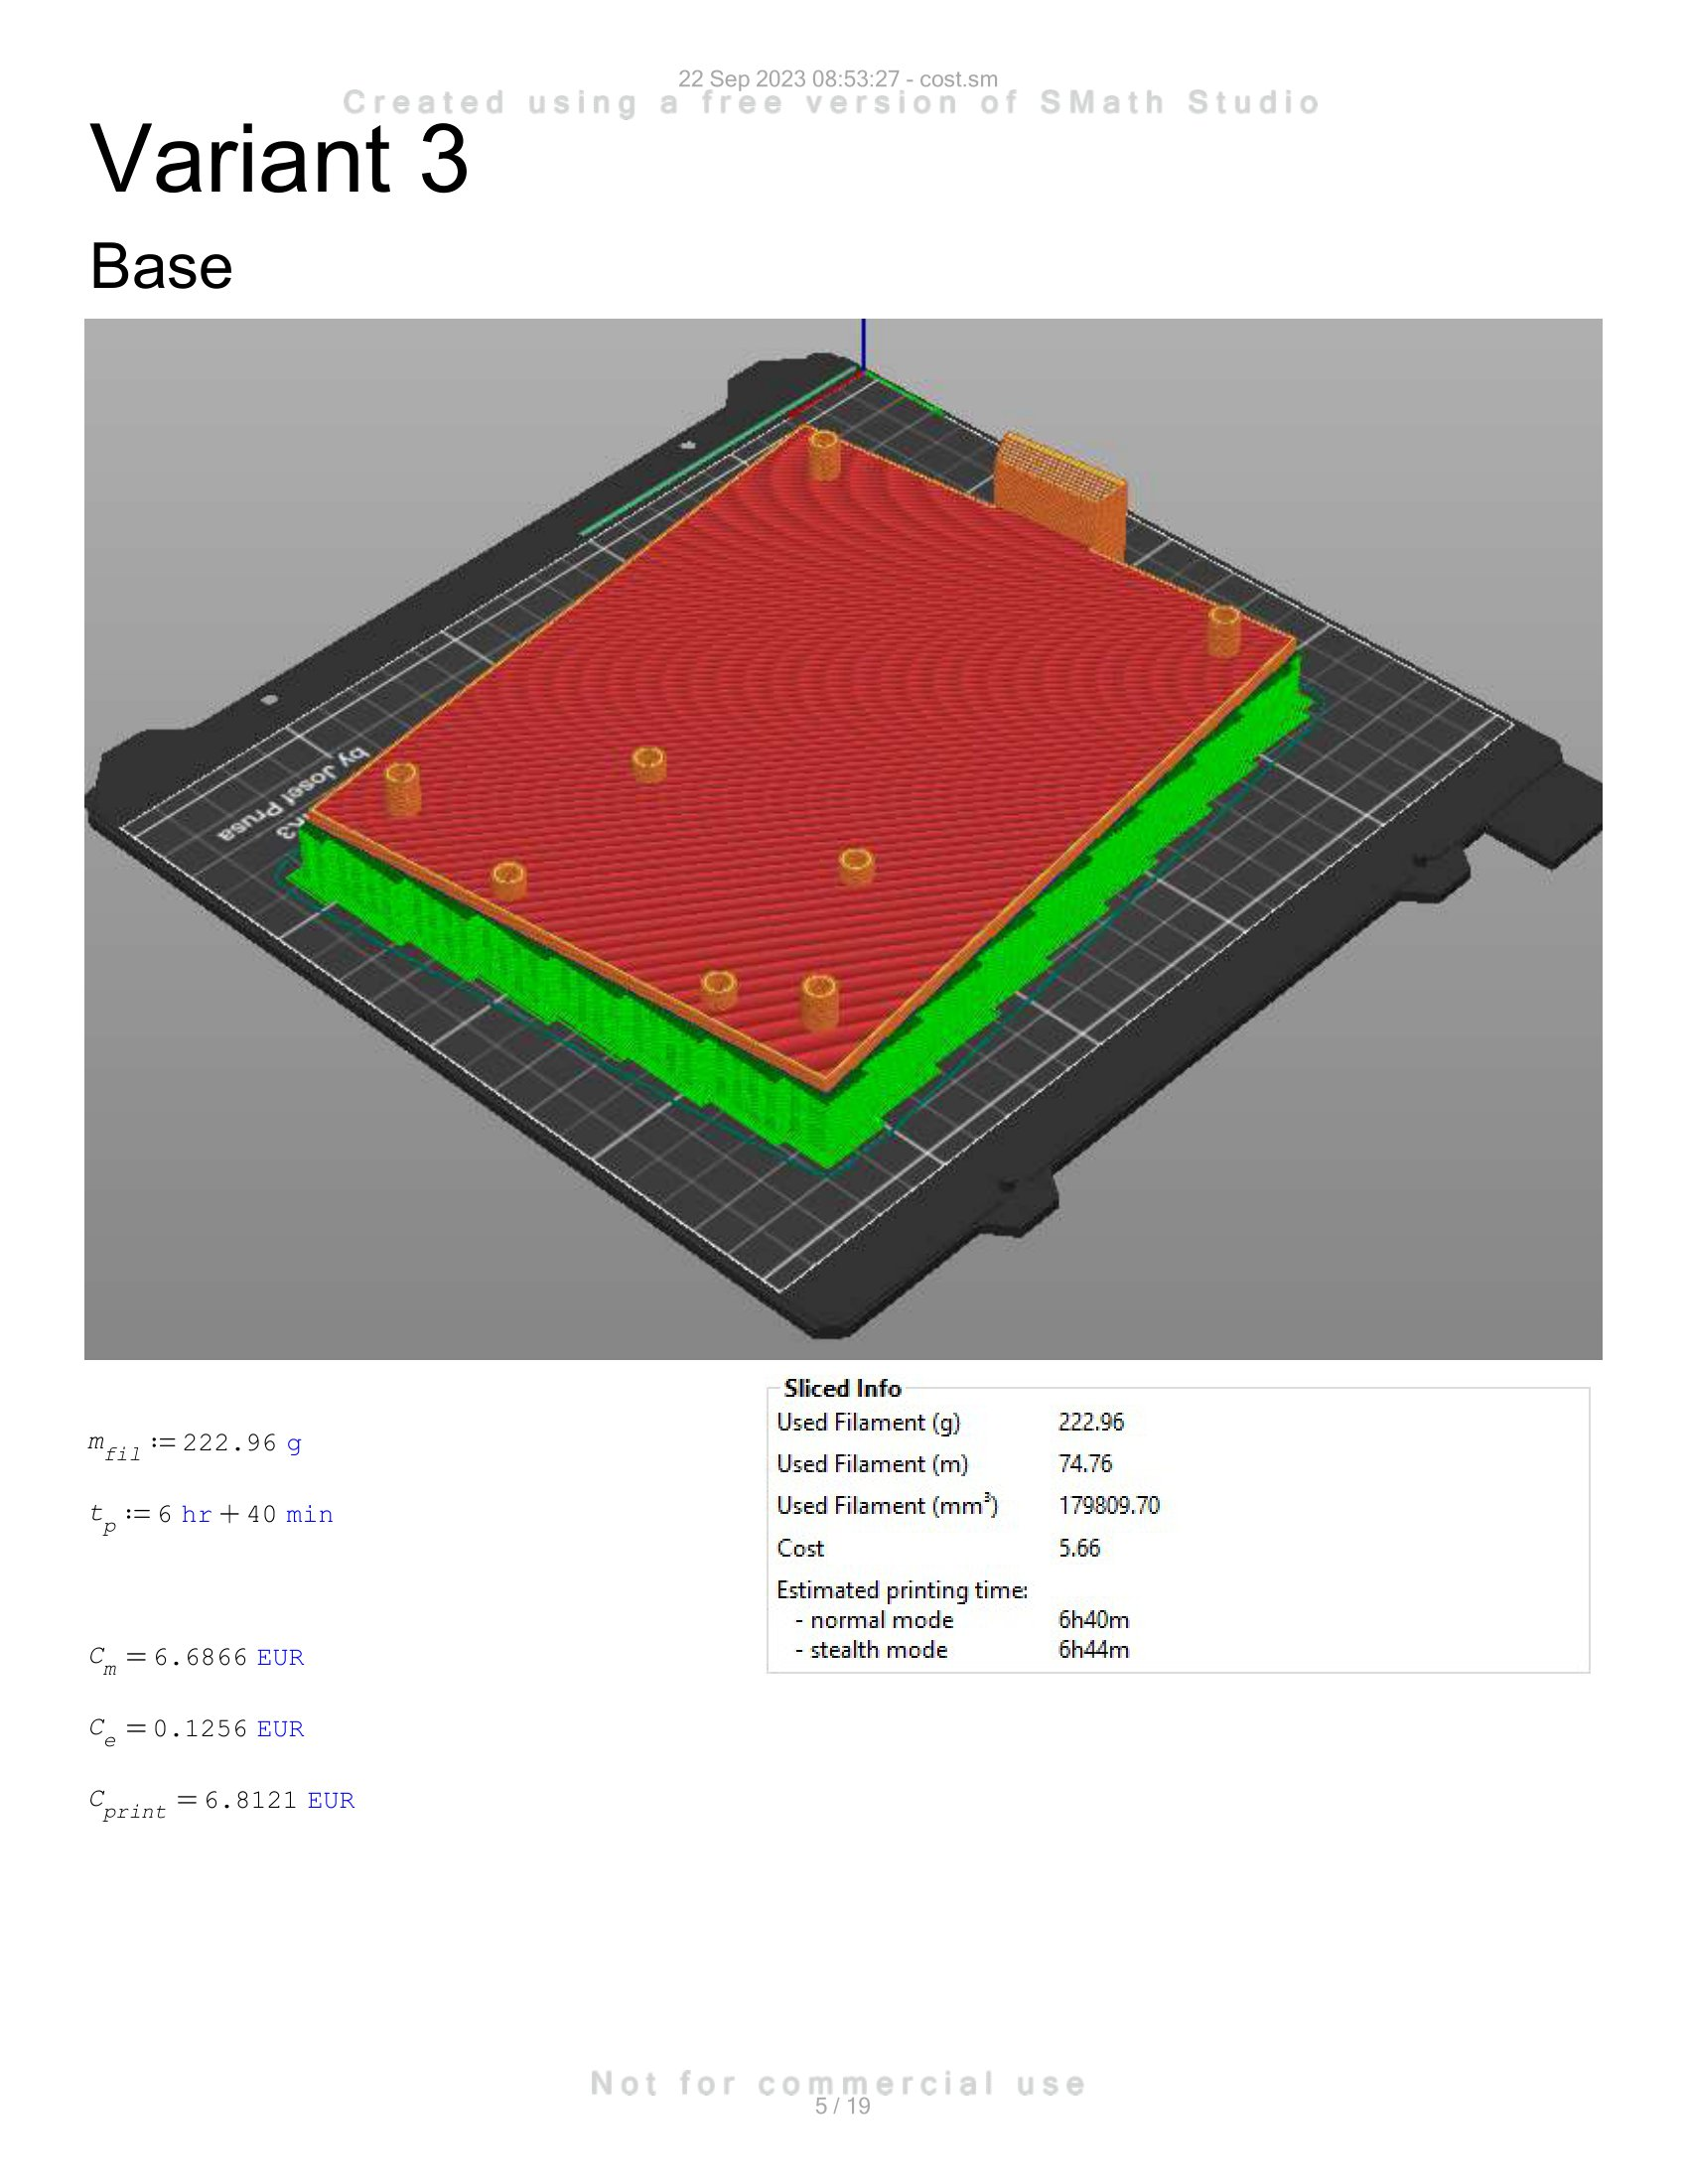
\includegraphics[width=\linewidth]{texs/appendix/data/costcalculation/cost1-05.jpg}
    \caption{Cost Calculation 5}
    \label{fig:cost-calculation-5}
\end{figure}

\begin{figure}[H]
    \centering
    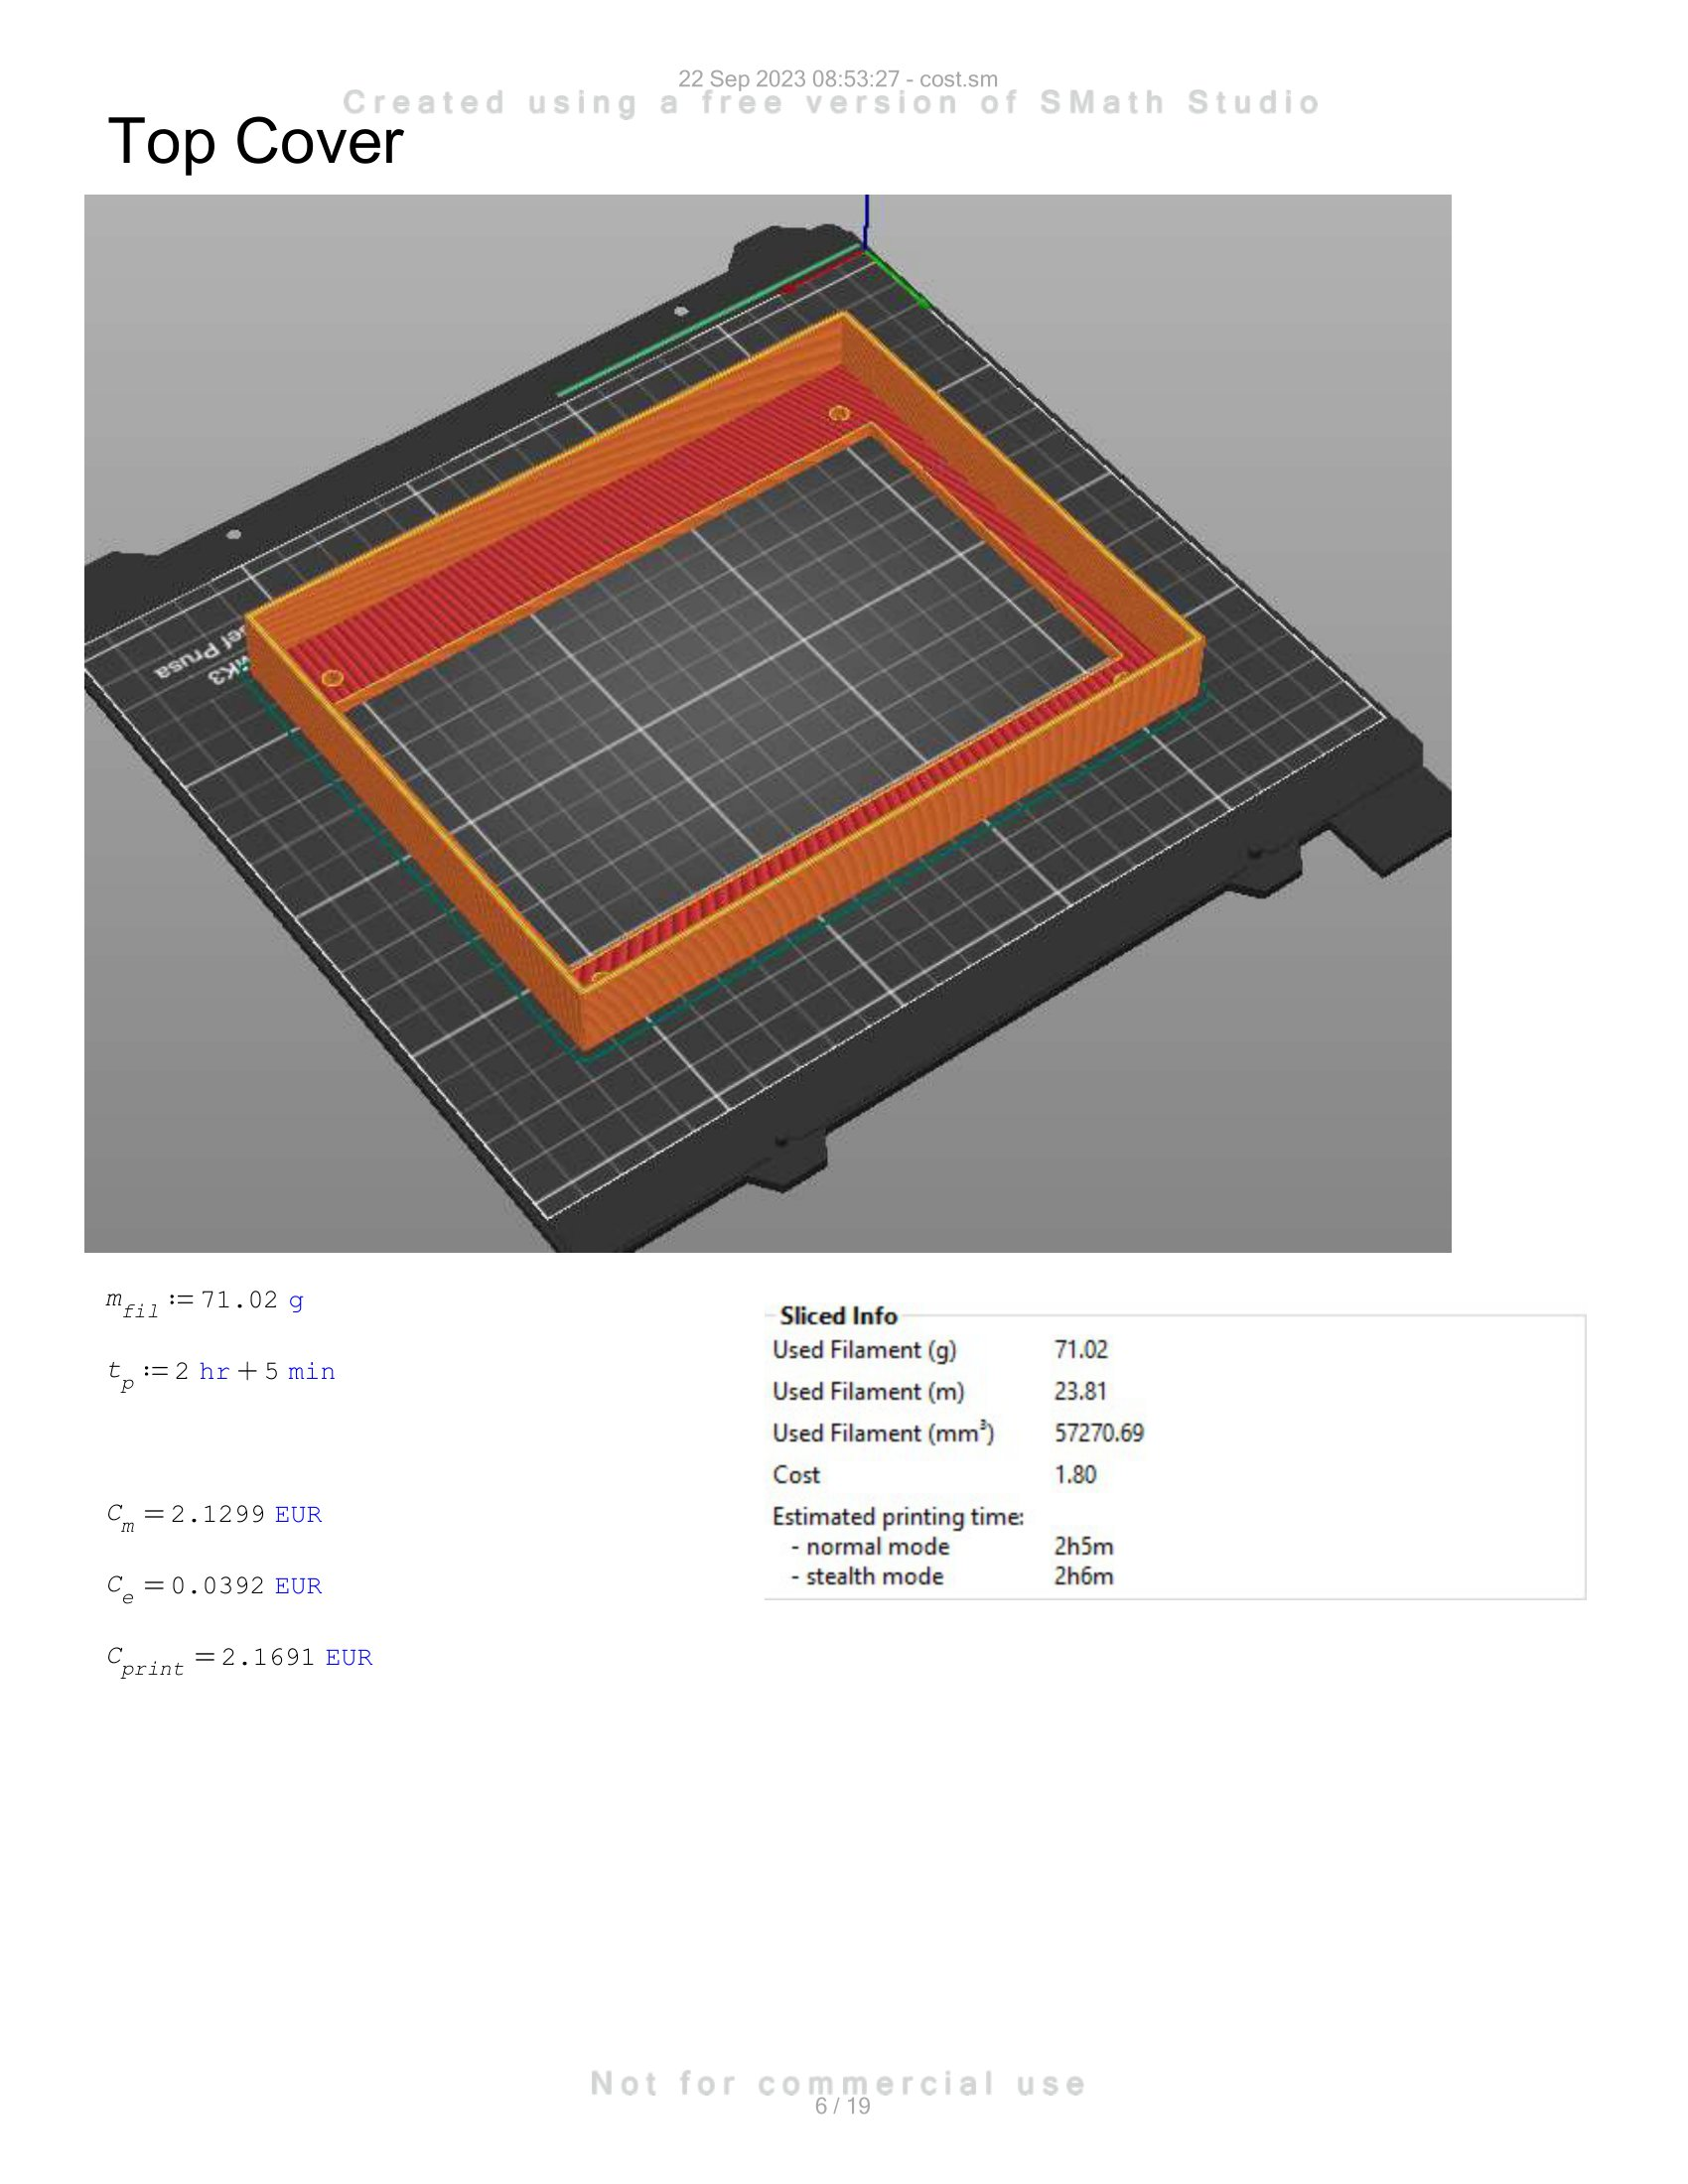
\includegraphics[width=\linewidth]{texs/appendix/data/costcalculation/cost1-06.jpg}
    \caption{Cost Calculation 6}
    \label{fig:cost-calculation-6}
\end{figure}

\begin{figure}[H]
    \centering
    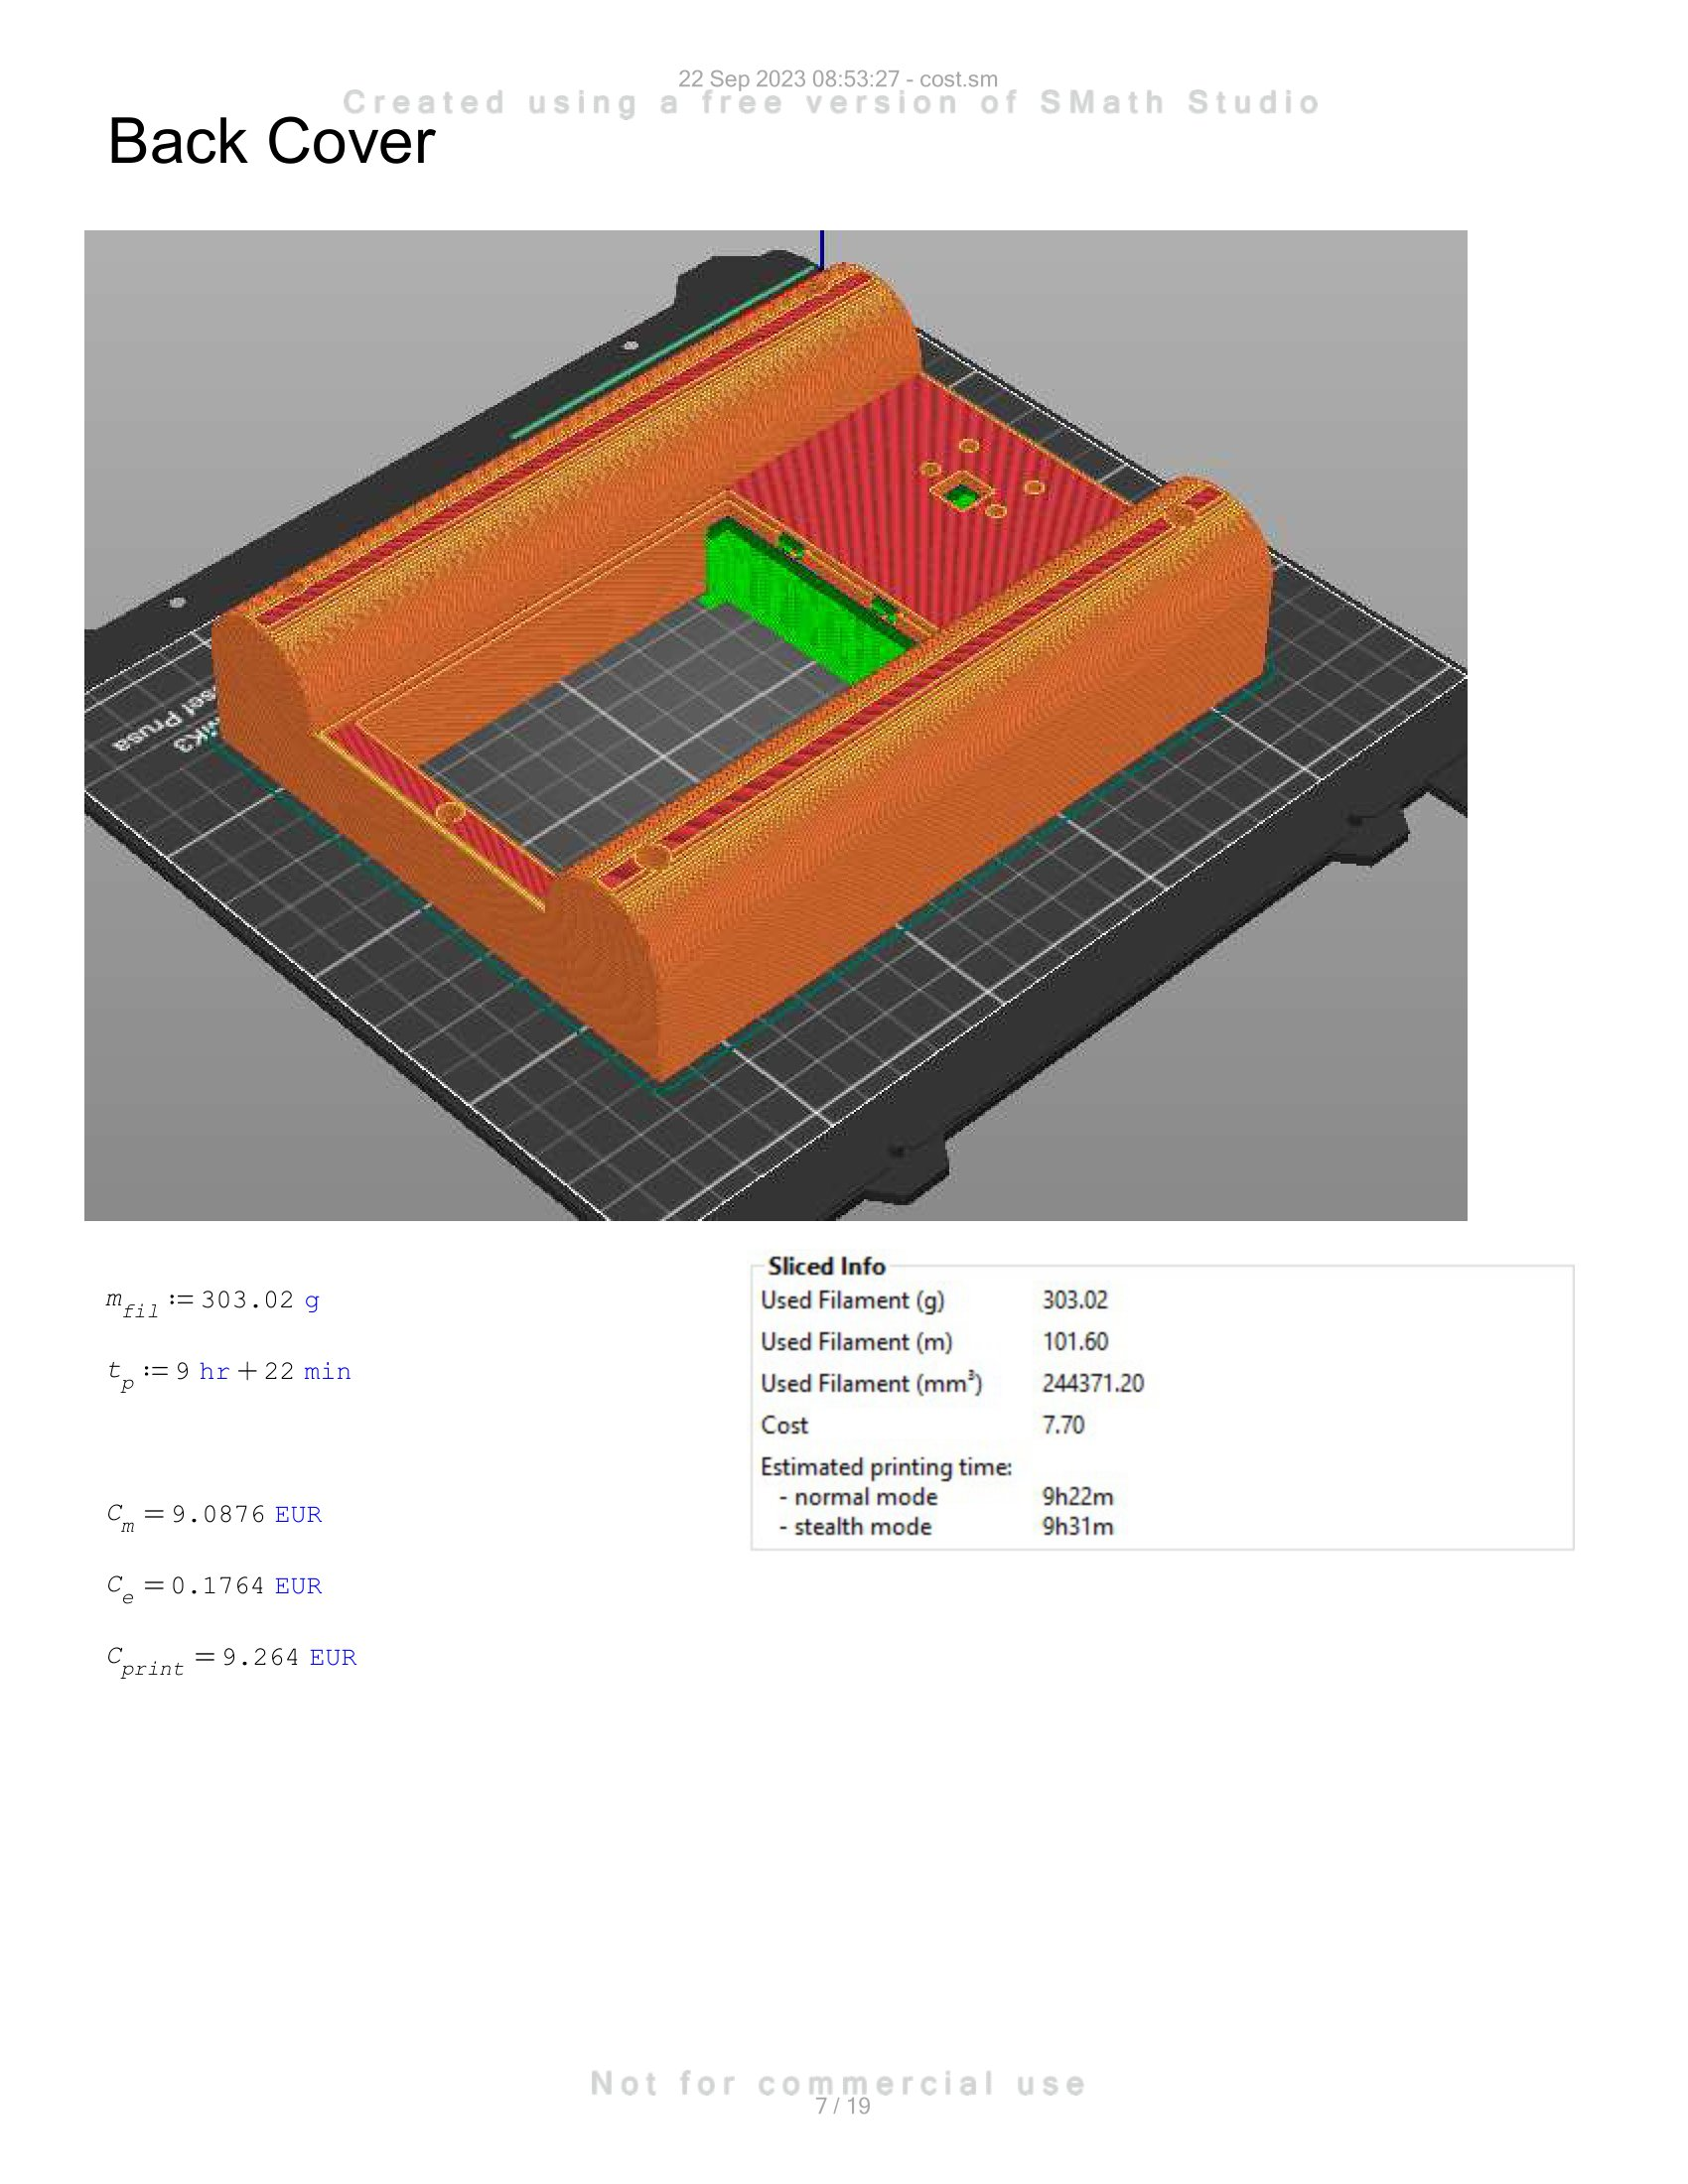
\includegraphics[width=\linewidth]{texs/appendix/data/costcalculation/cost1-07.jpg}
    \caption{Cost Calculation 7}
    \label{fig:cost-calculation-7}
\end{figure}

\begin{figure}[H]
    \centering
    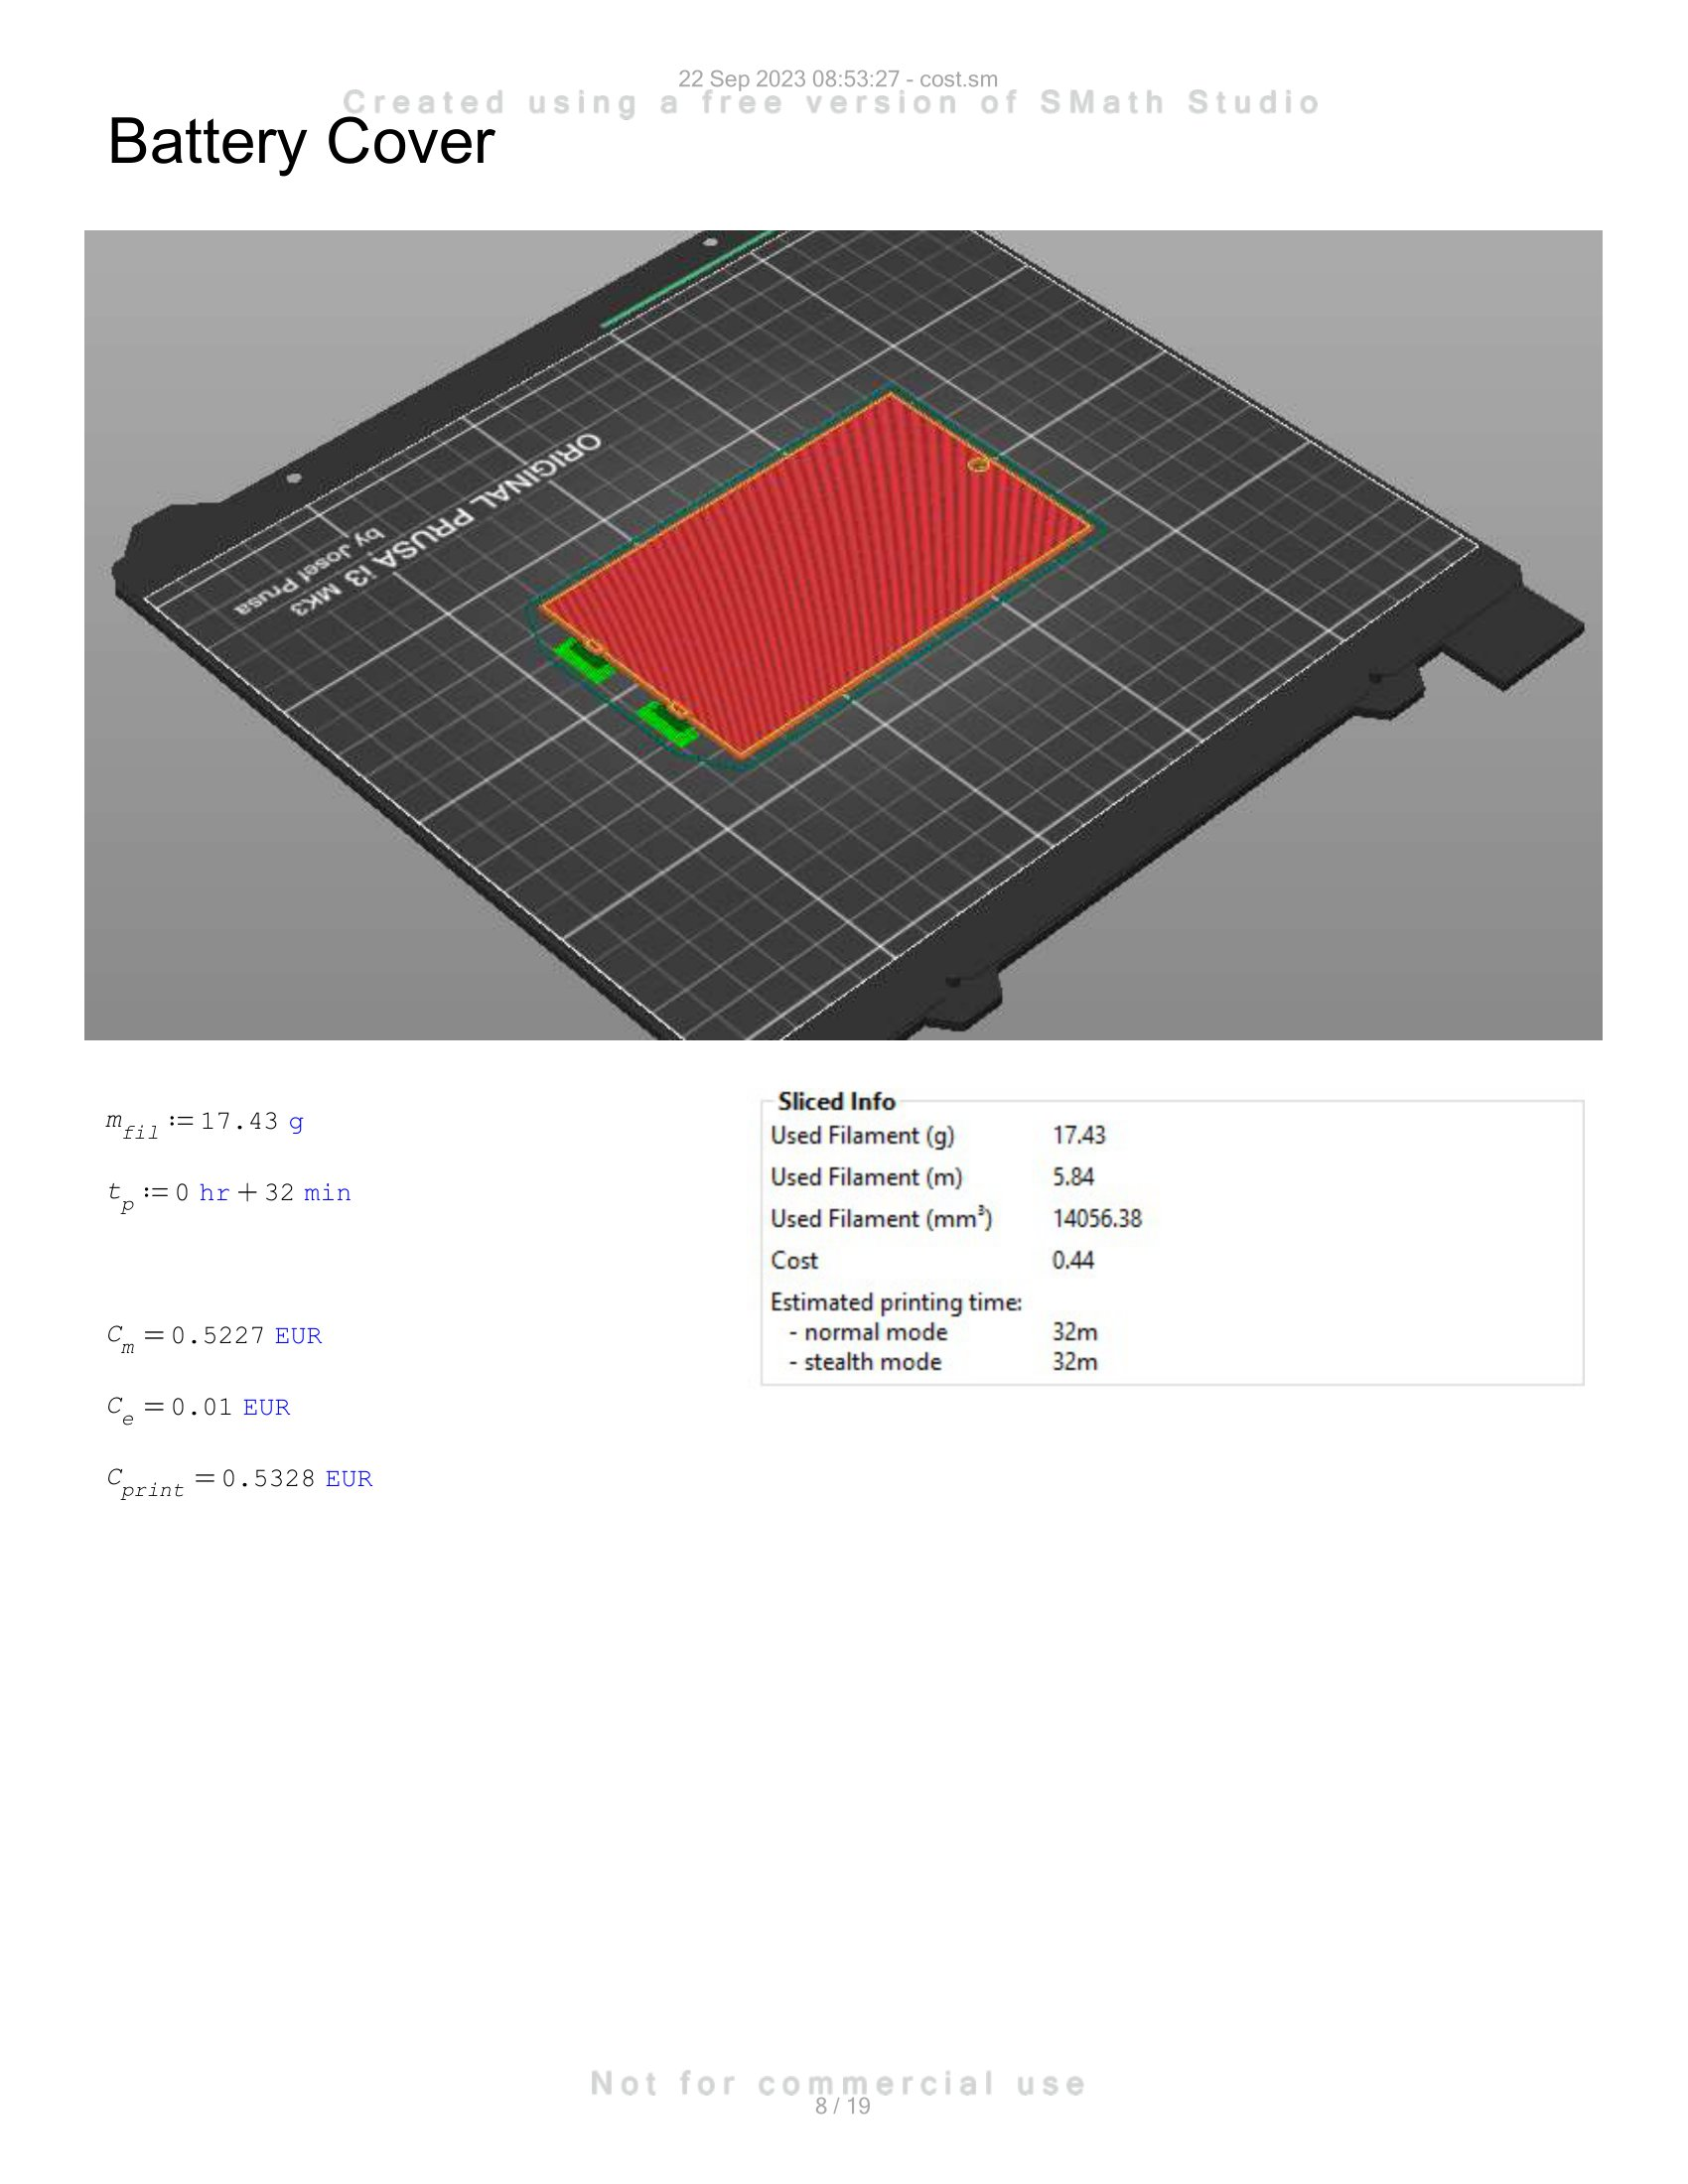
\includegraphics[width=\linewidth]{texs/appendix/data/costcalculation/cost1-08.jpg}
    \caption{Cost Calculation 8}
    \label{fig:cost-calculation-8}
\end{figure}

\begin{figure}[H]
    \centering
    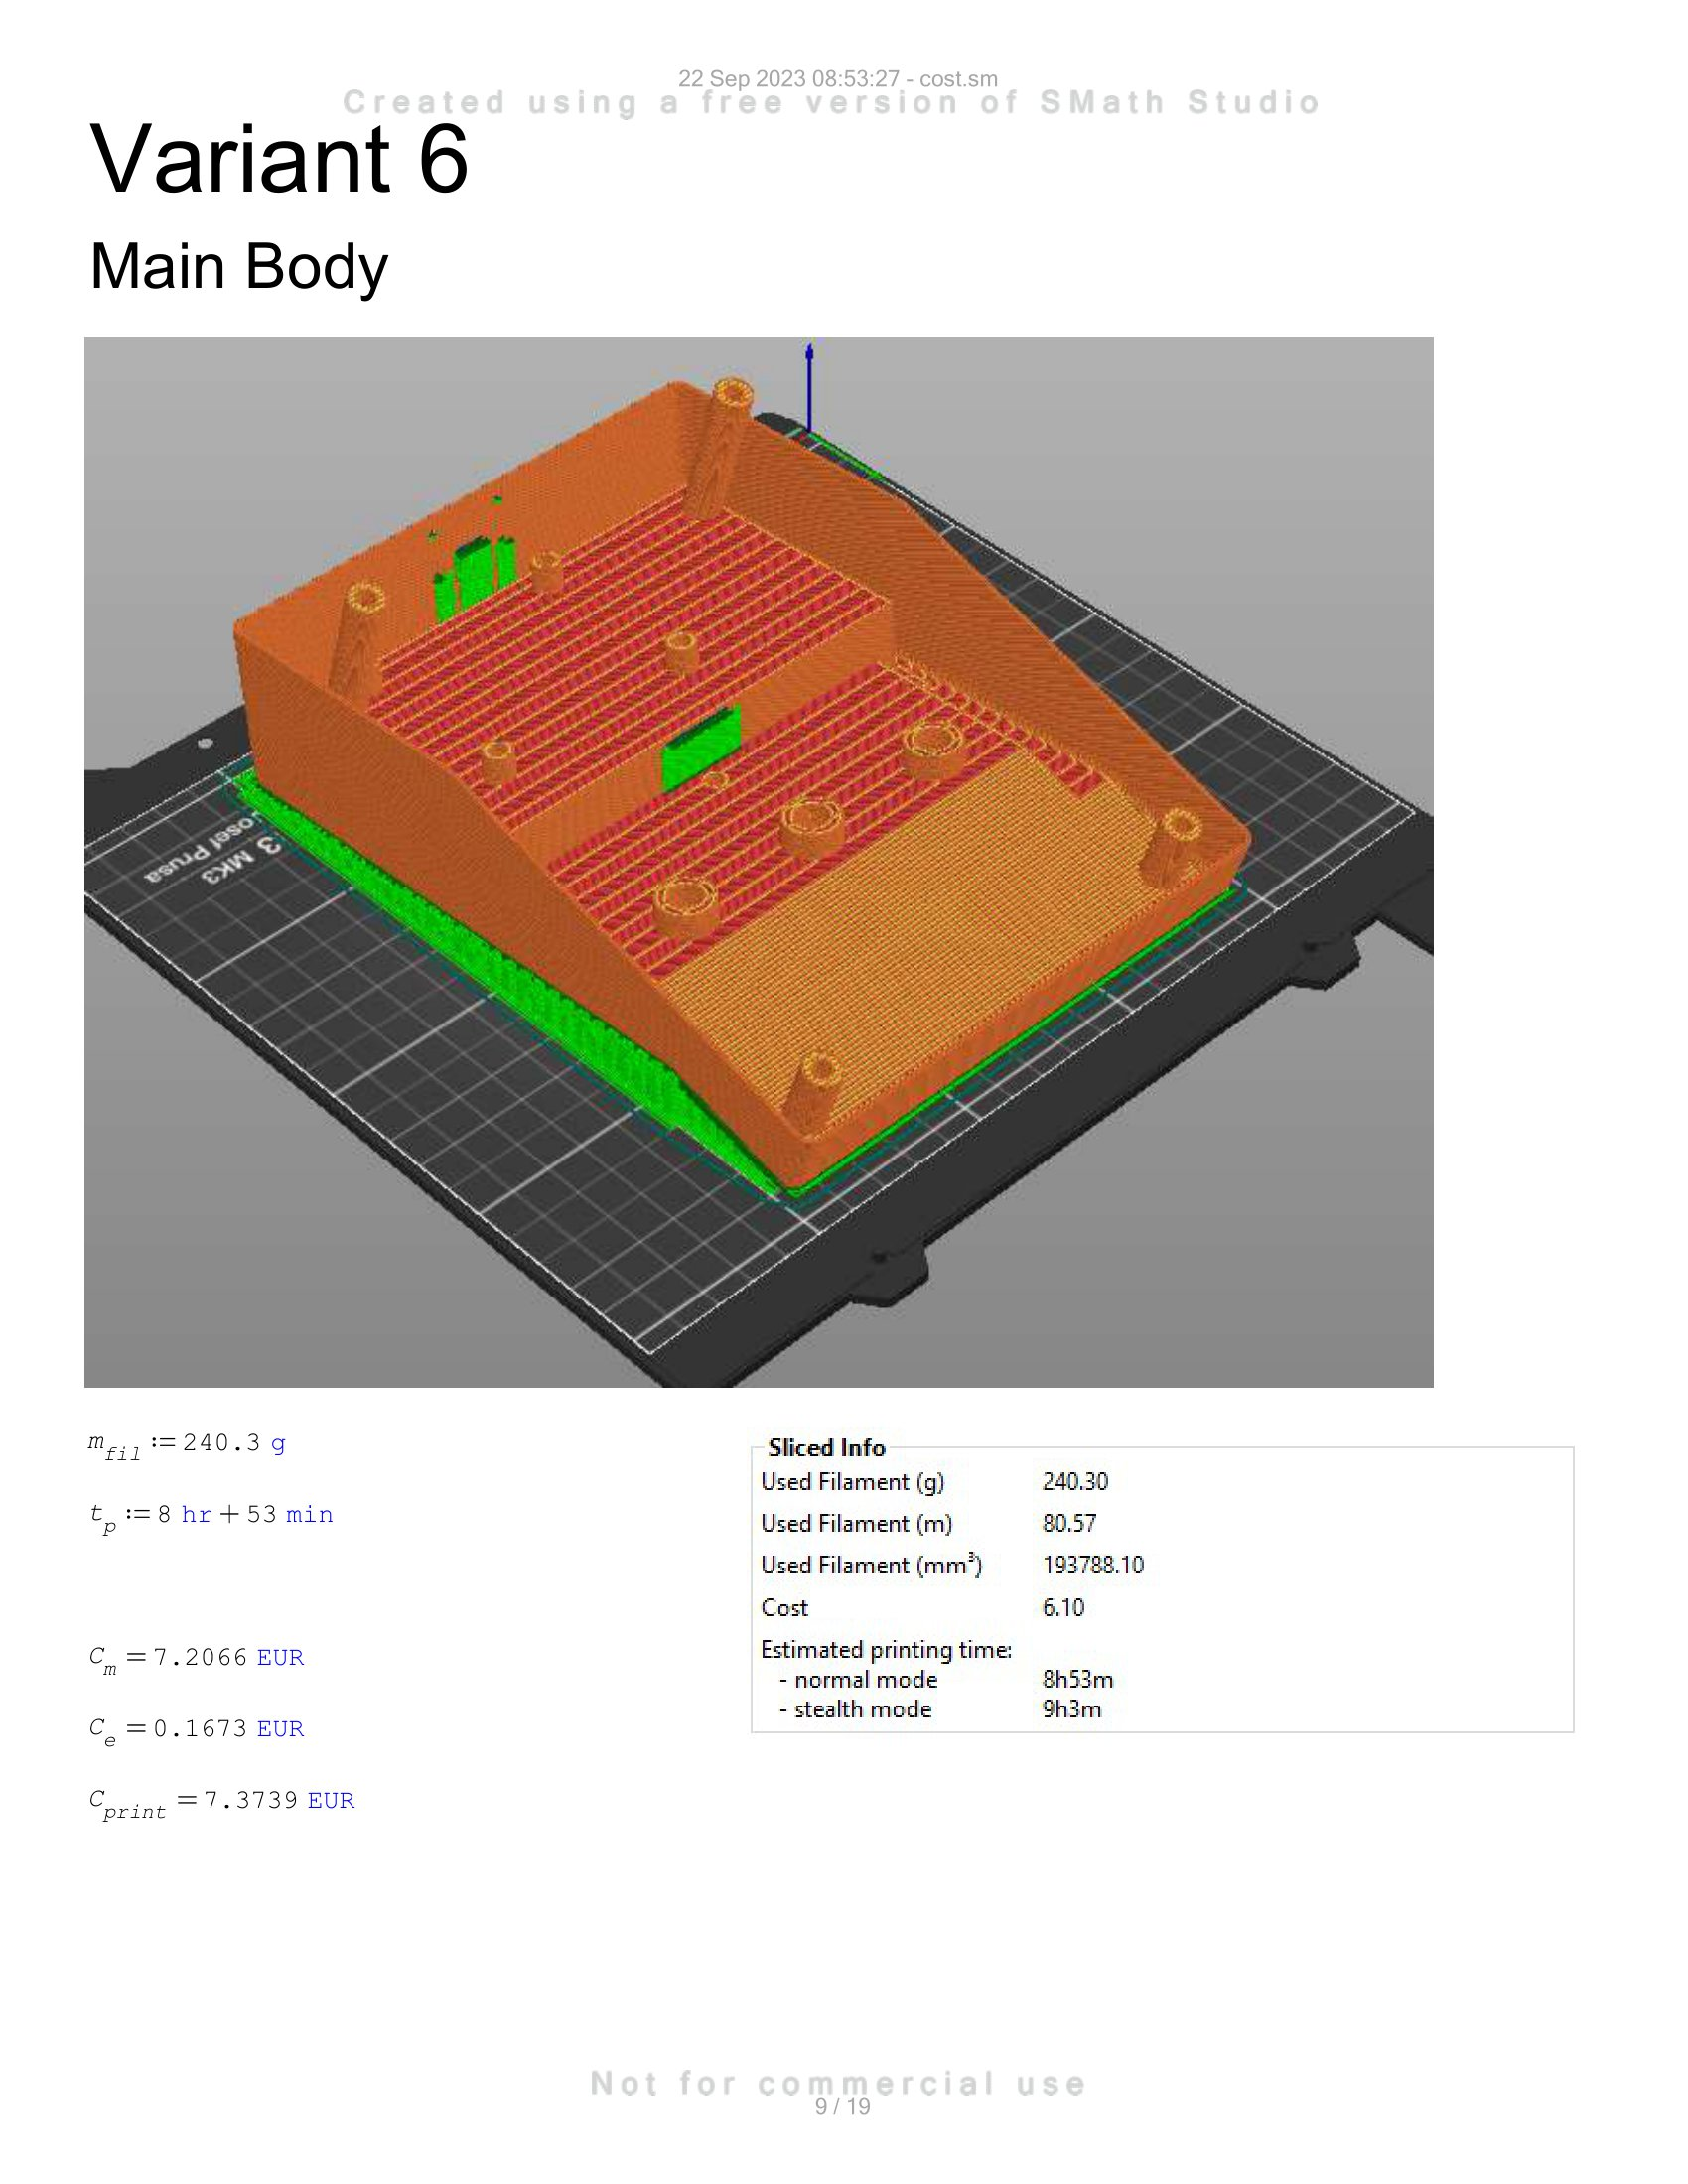
\includegraphics[width=\linewidth]{texs/appendix/data/costcalculation/cost1-09.jpg}
    \caption{Cost Calculation 9}
    \label{fig:cost-calculation-9}
\end{figure}

\begin{figure}[H]
    \centering
    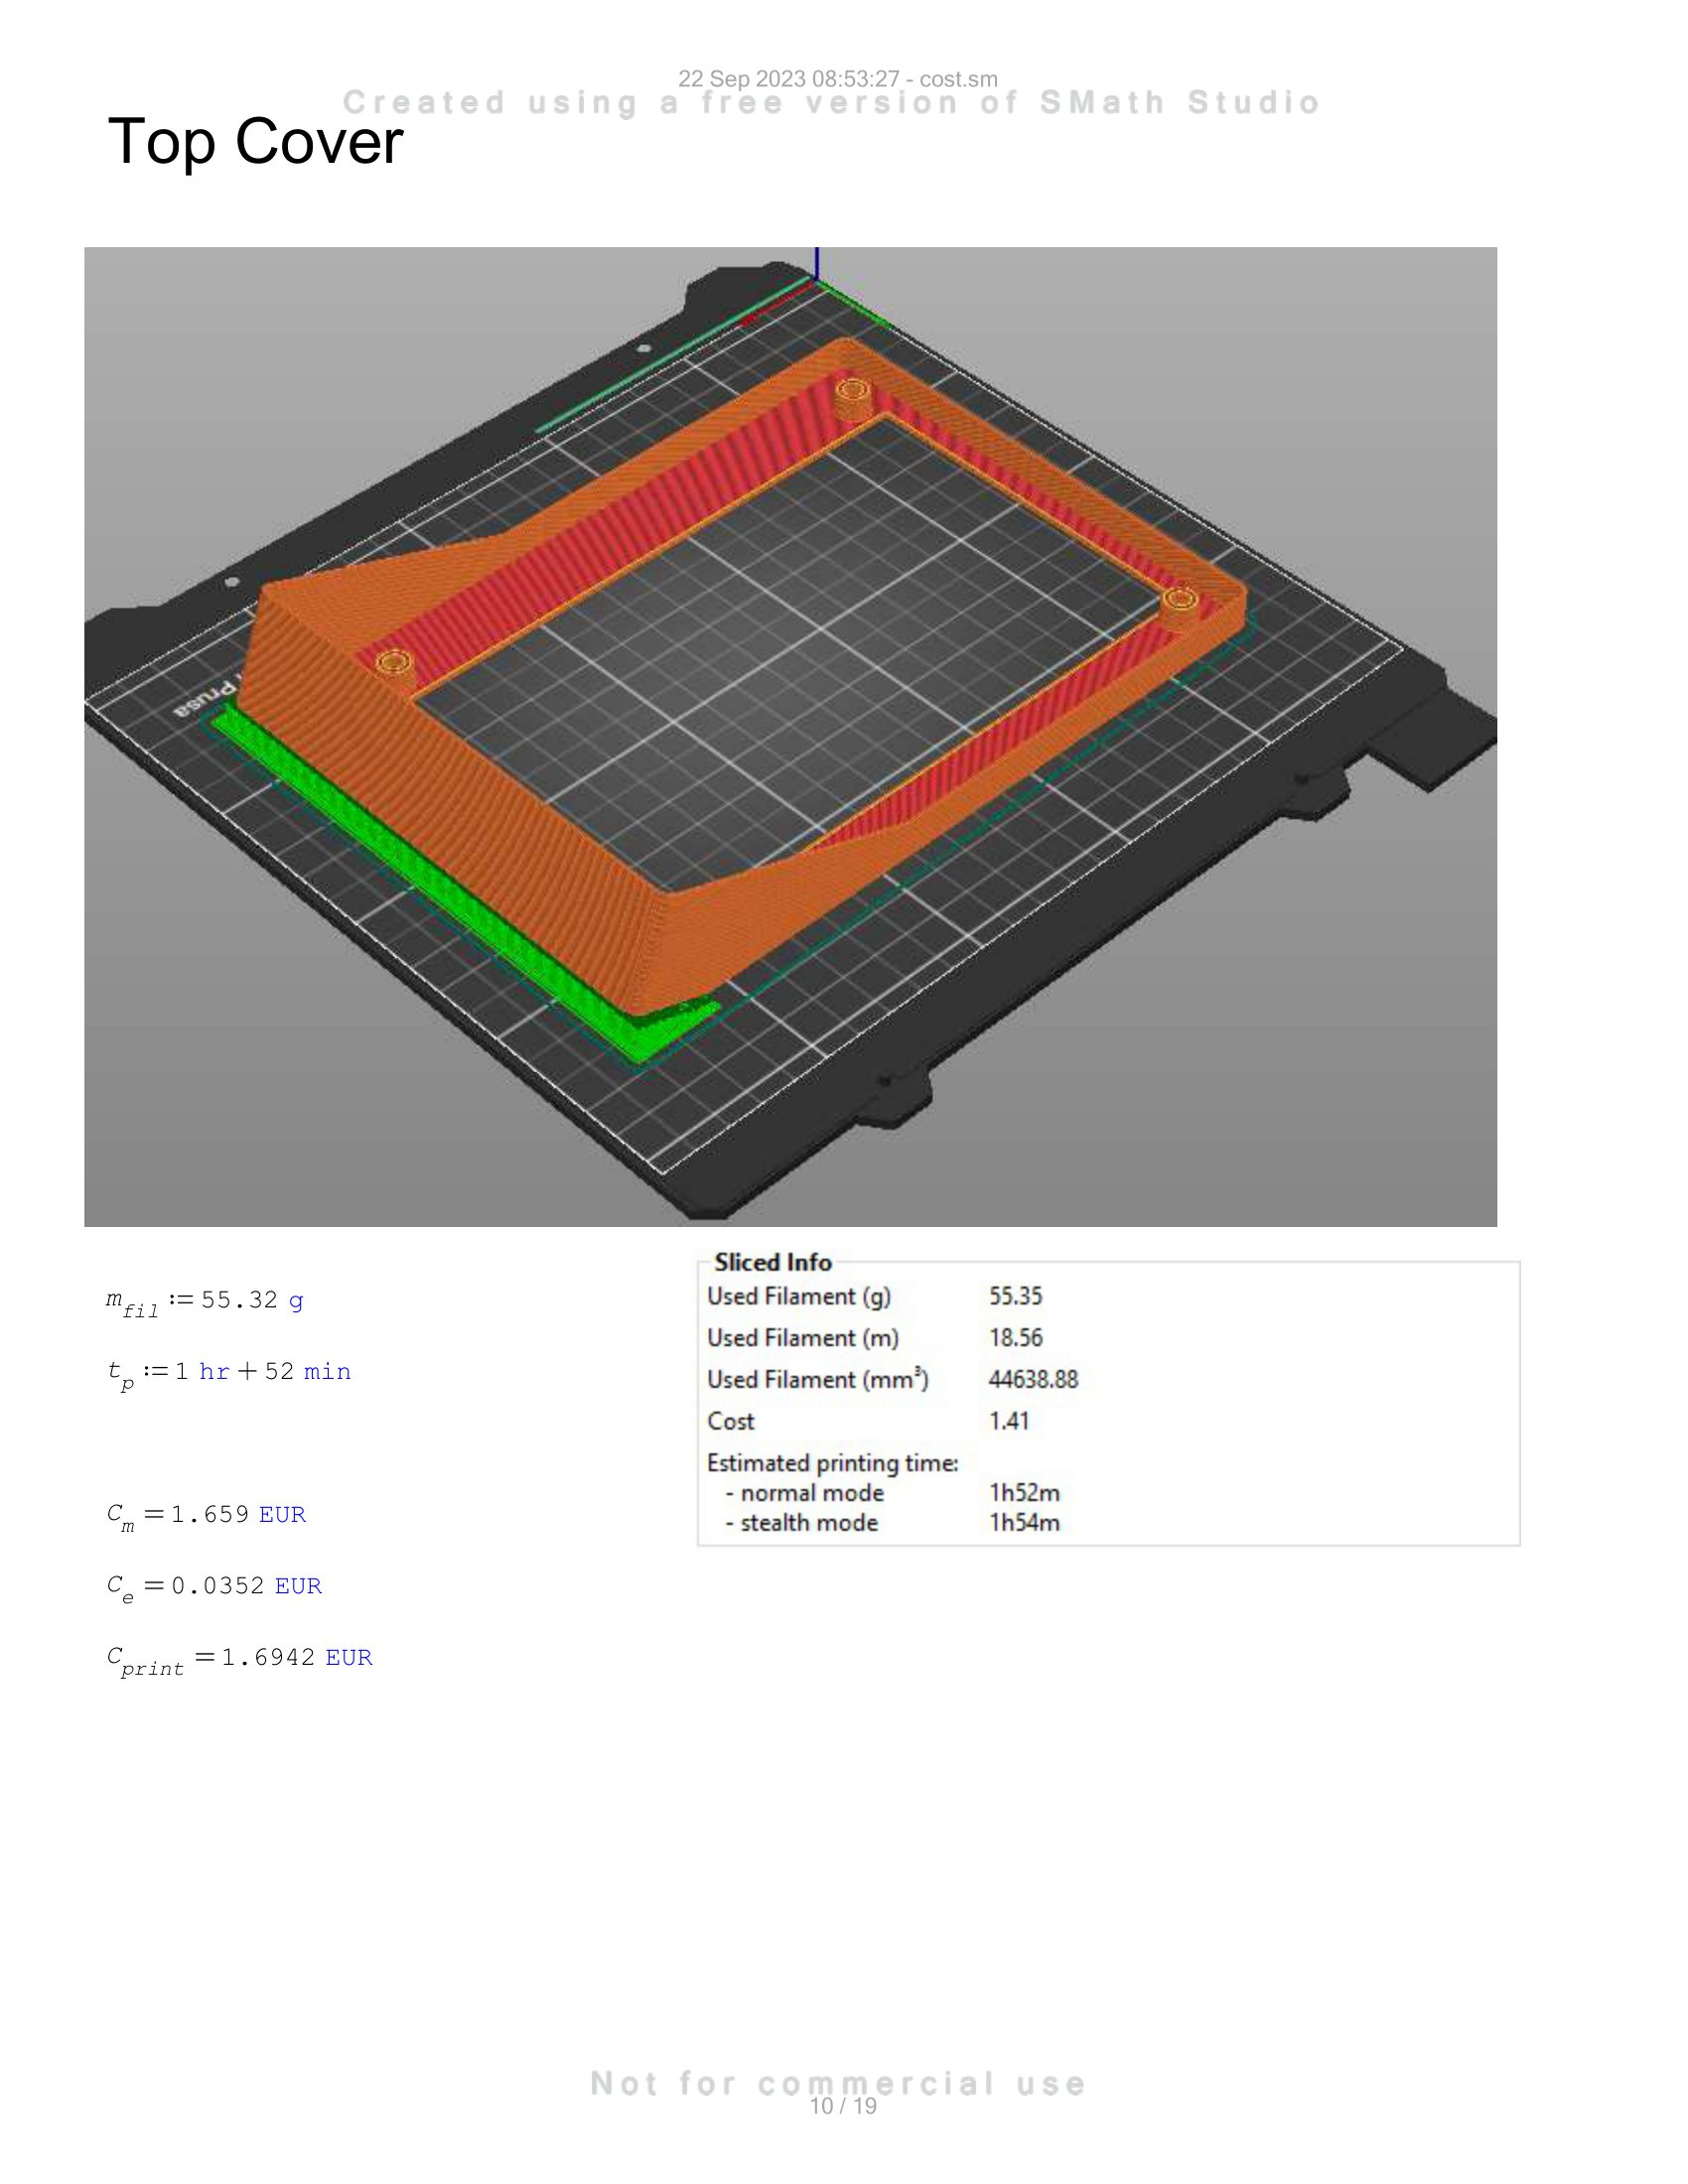
\includegraphics[width=\linewidth]{texs/appendix/data/costcalculation/cost1-10.jpg}
    \caption{Cost Calculation 10}
    \label{fig:cost-calculation-10}
\end{figure}

\begin{figure}[H]
    \centering
    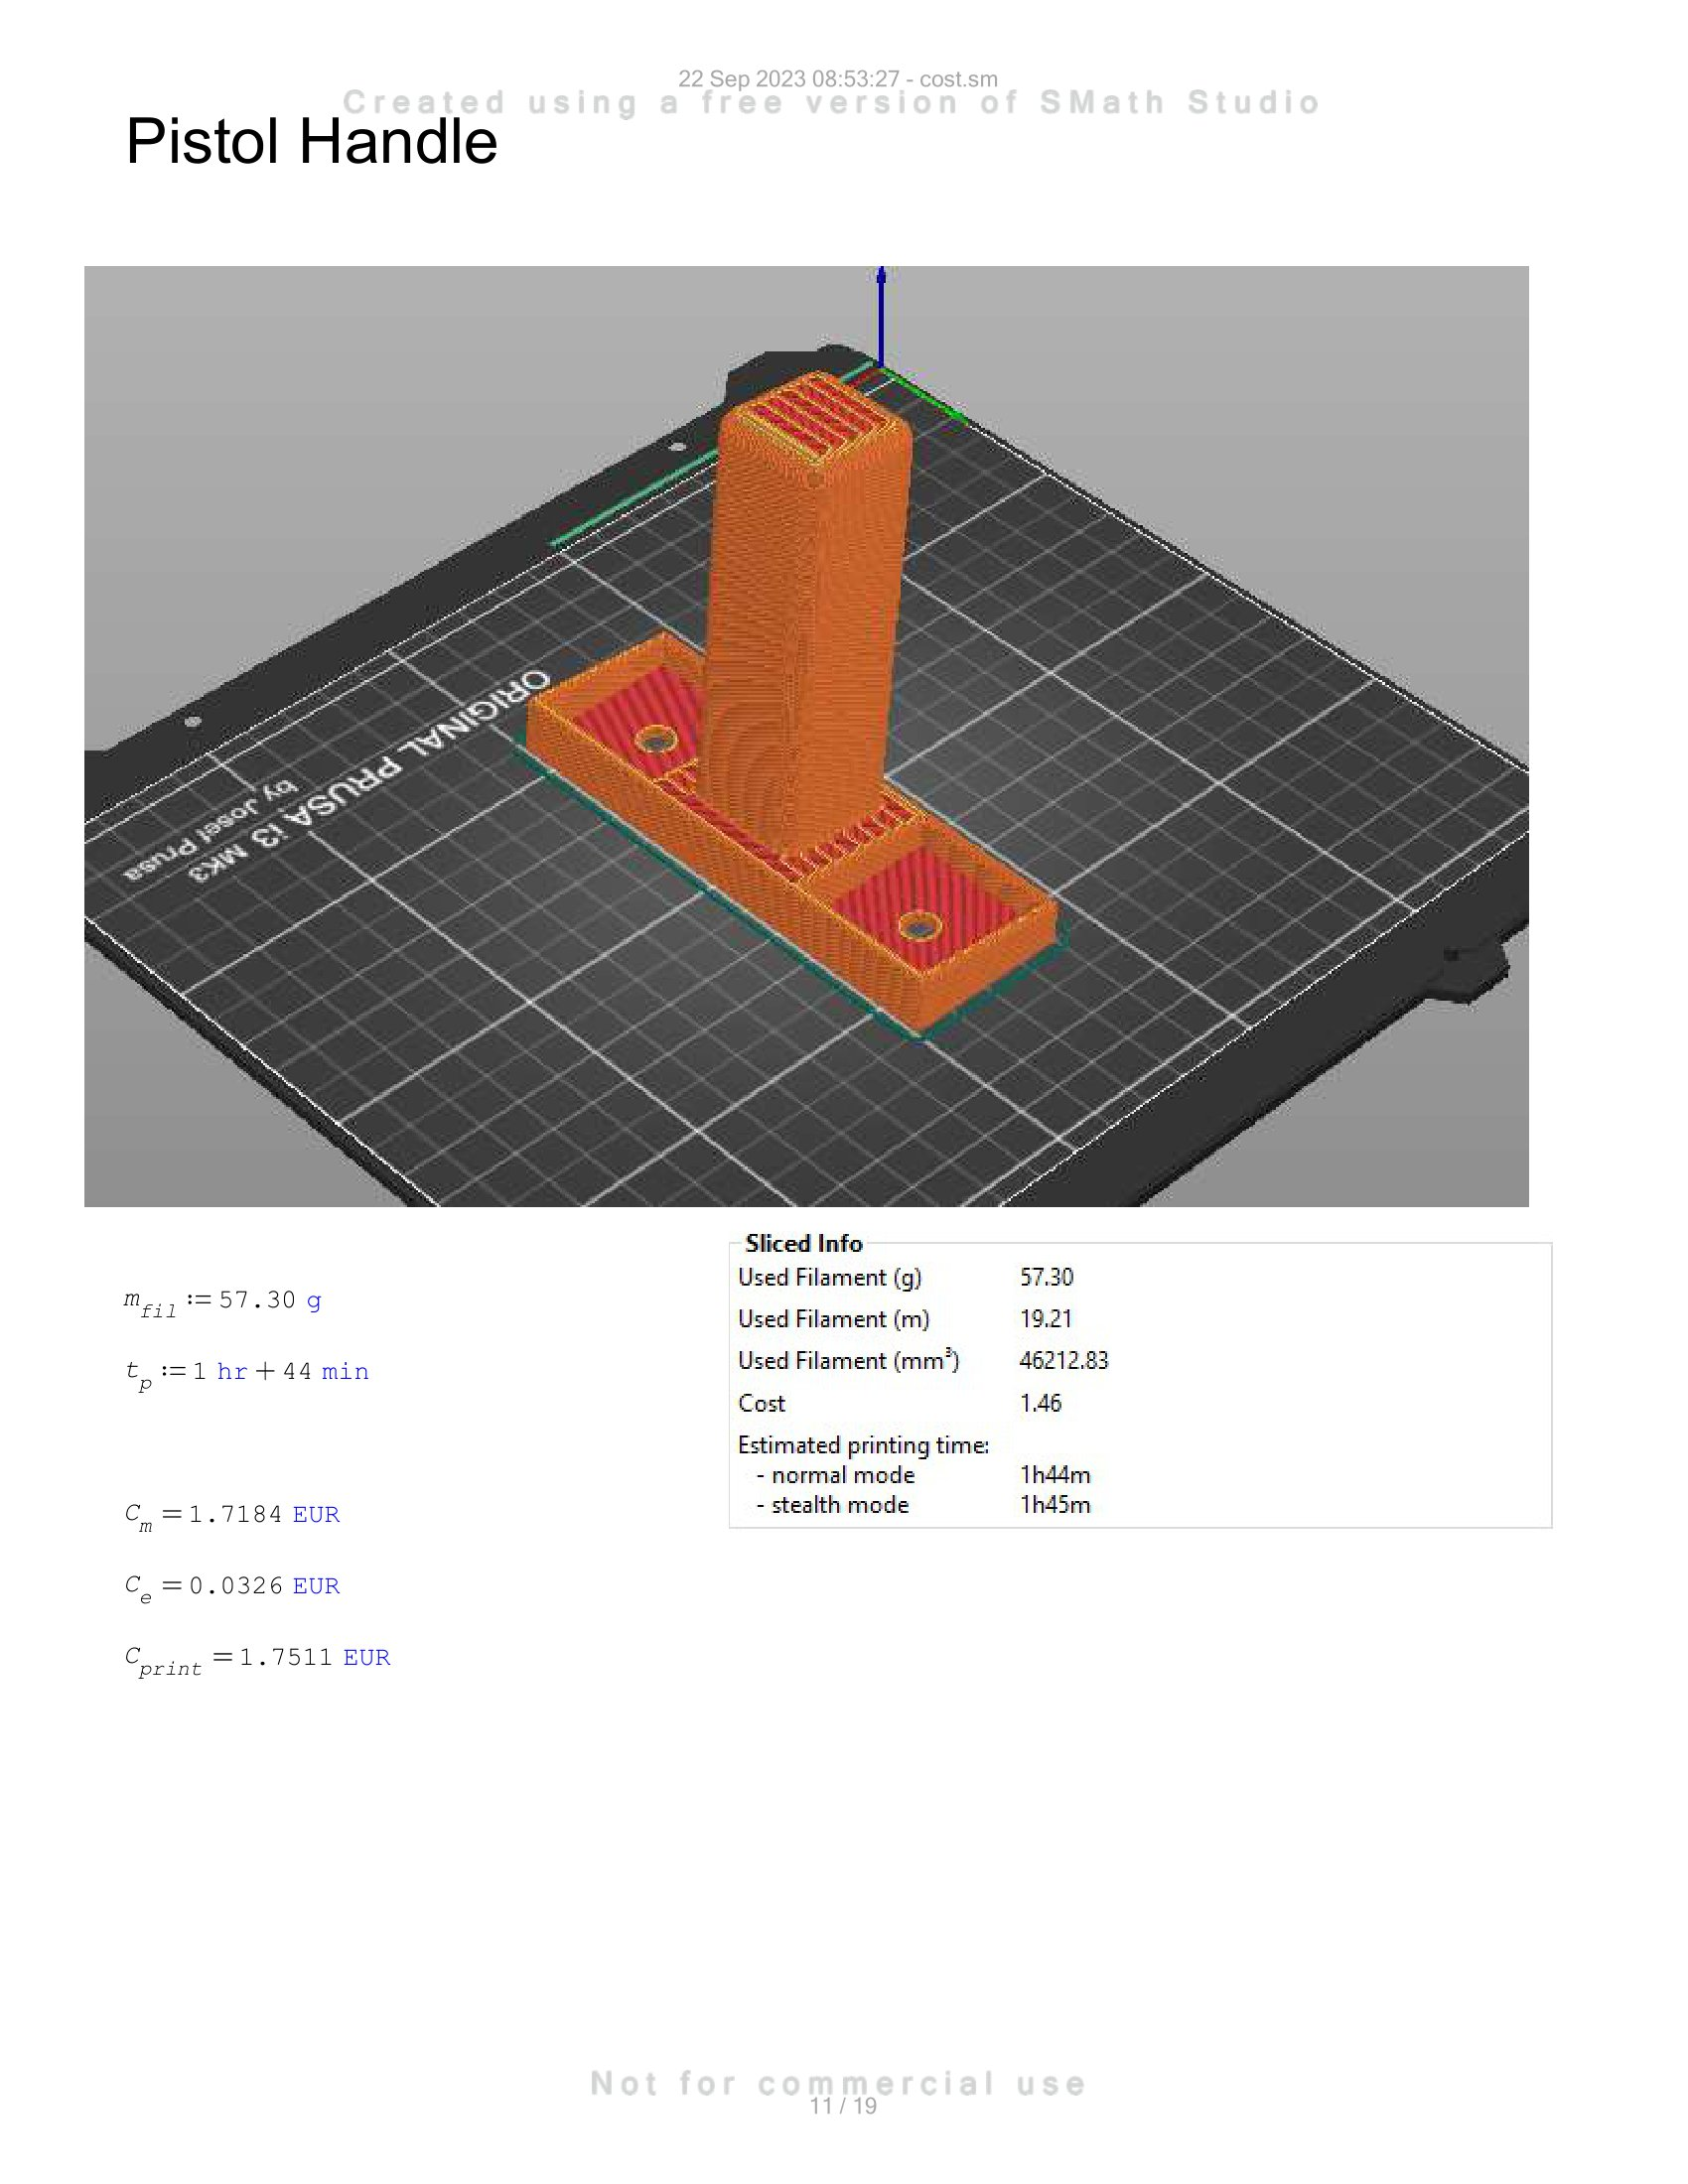
\includegraphics[width=\linewidth]{texs/appendix/data/costcalculation/cost1-11.jpg}
    \caption{Cost Calculation 11}
    \label{fig:cost-calculation-11}
\end{figure}

\begin{figure}[H]
    \centering
    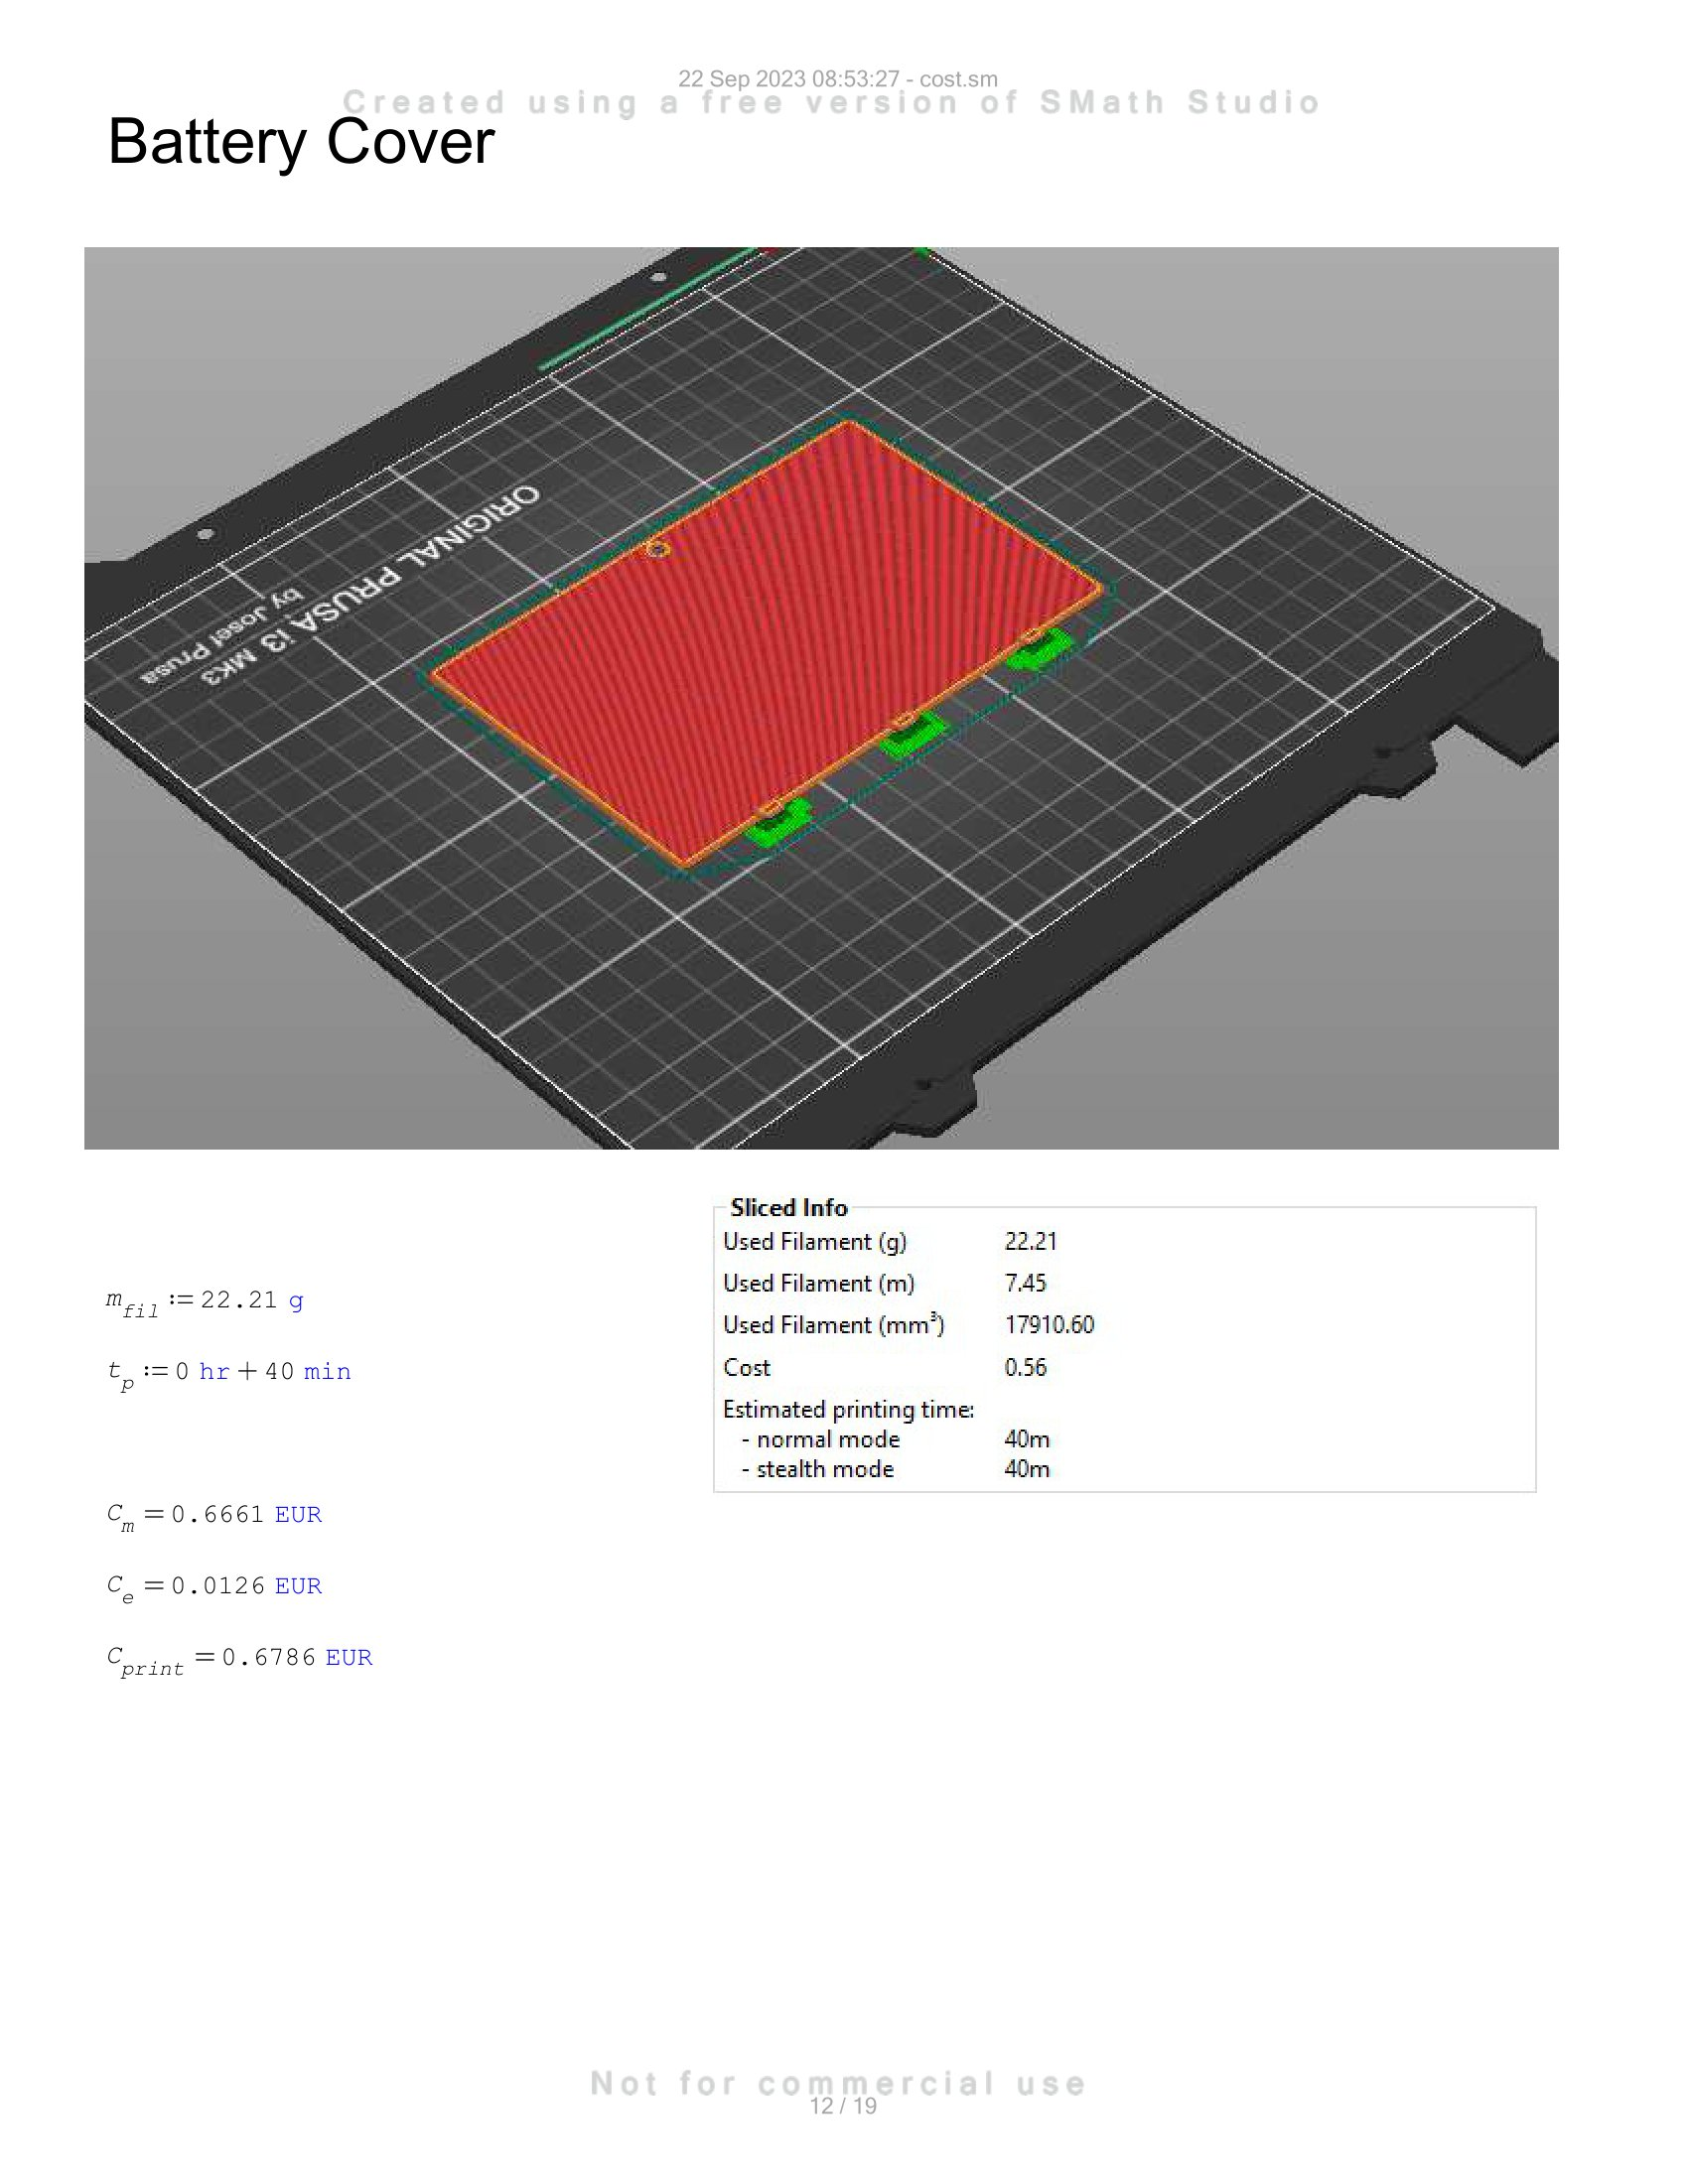
\includegraphics[width=\linewidth]{texs/appendix/data/costcalculation/cost1-12.jpg}
    \caption{Cost Calculation 12}
    \label{fig:cost-calculation-12}
\end{figure}

\begin{figure}[H]
    \centering
    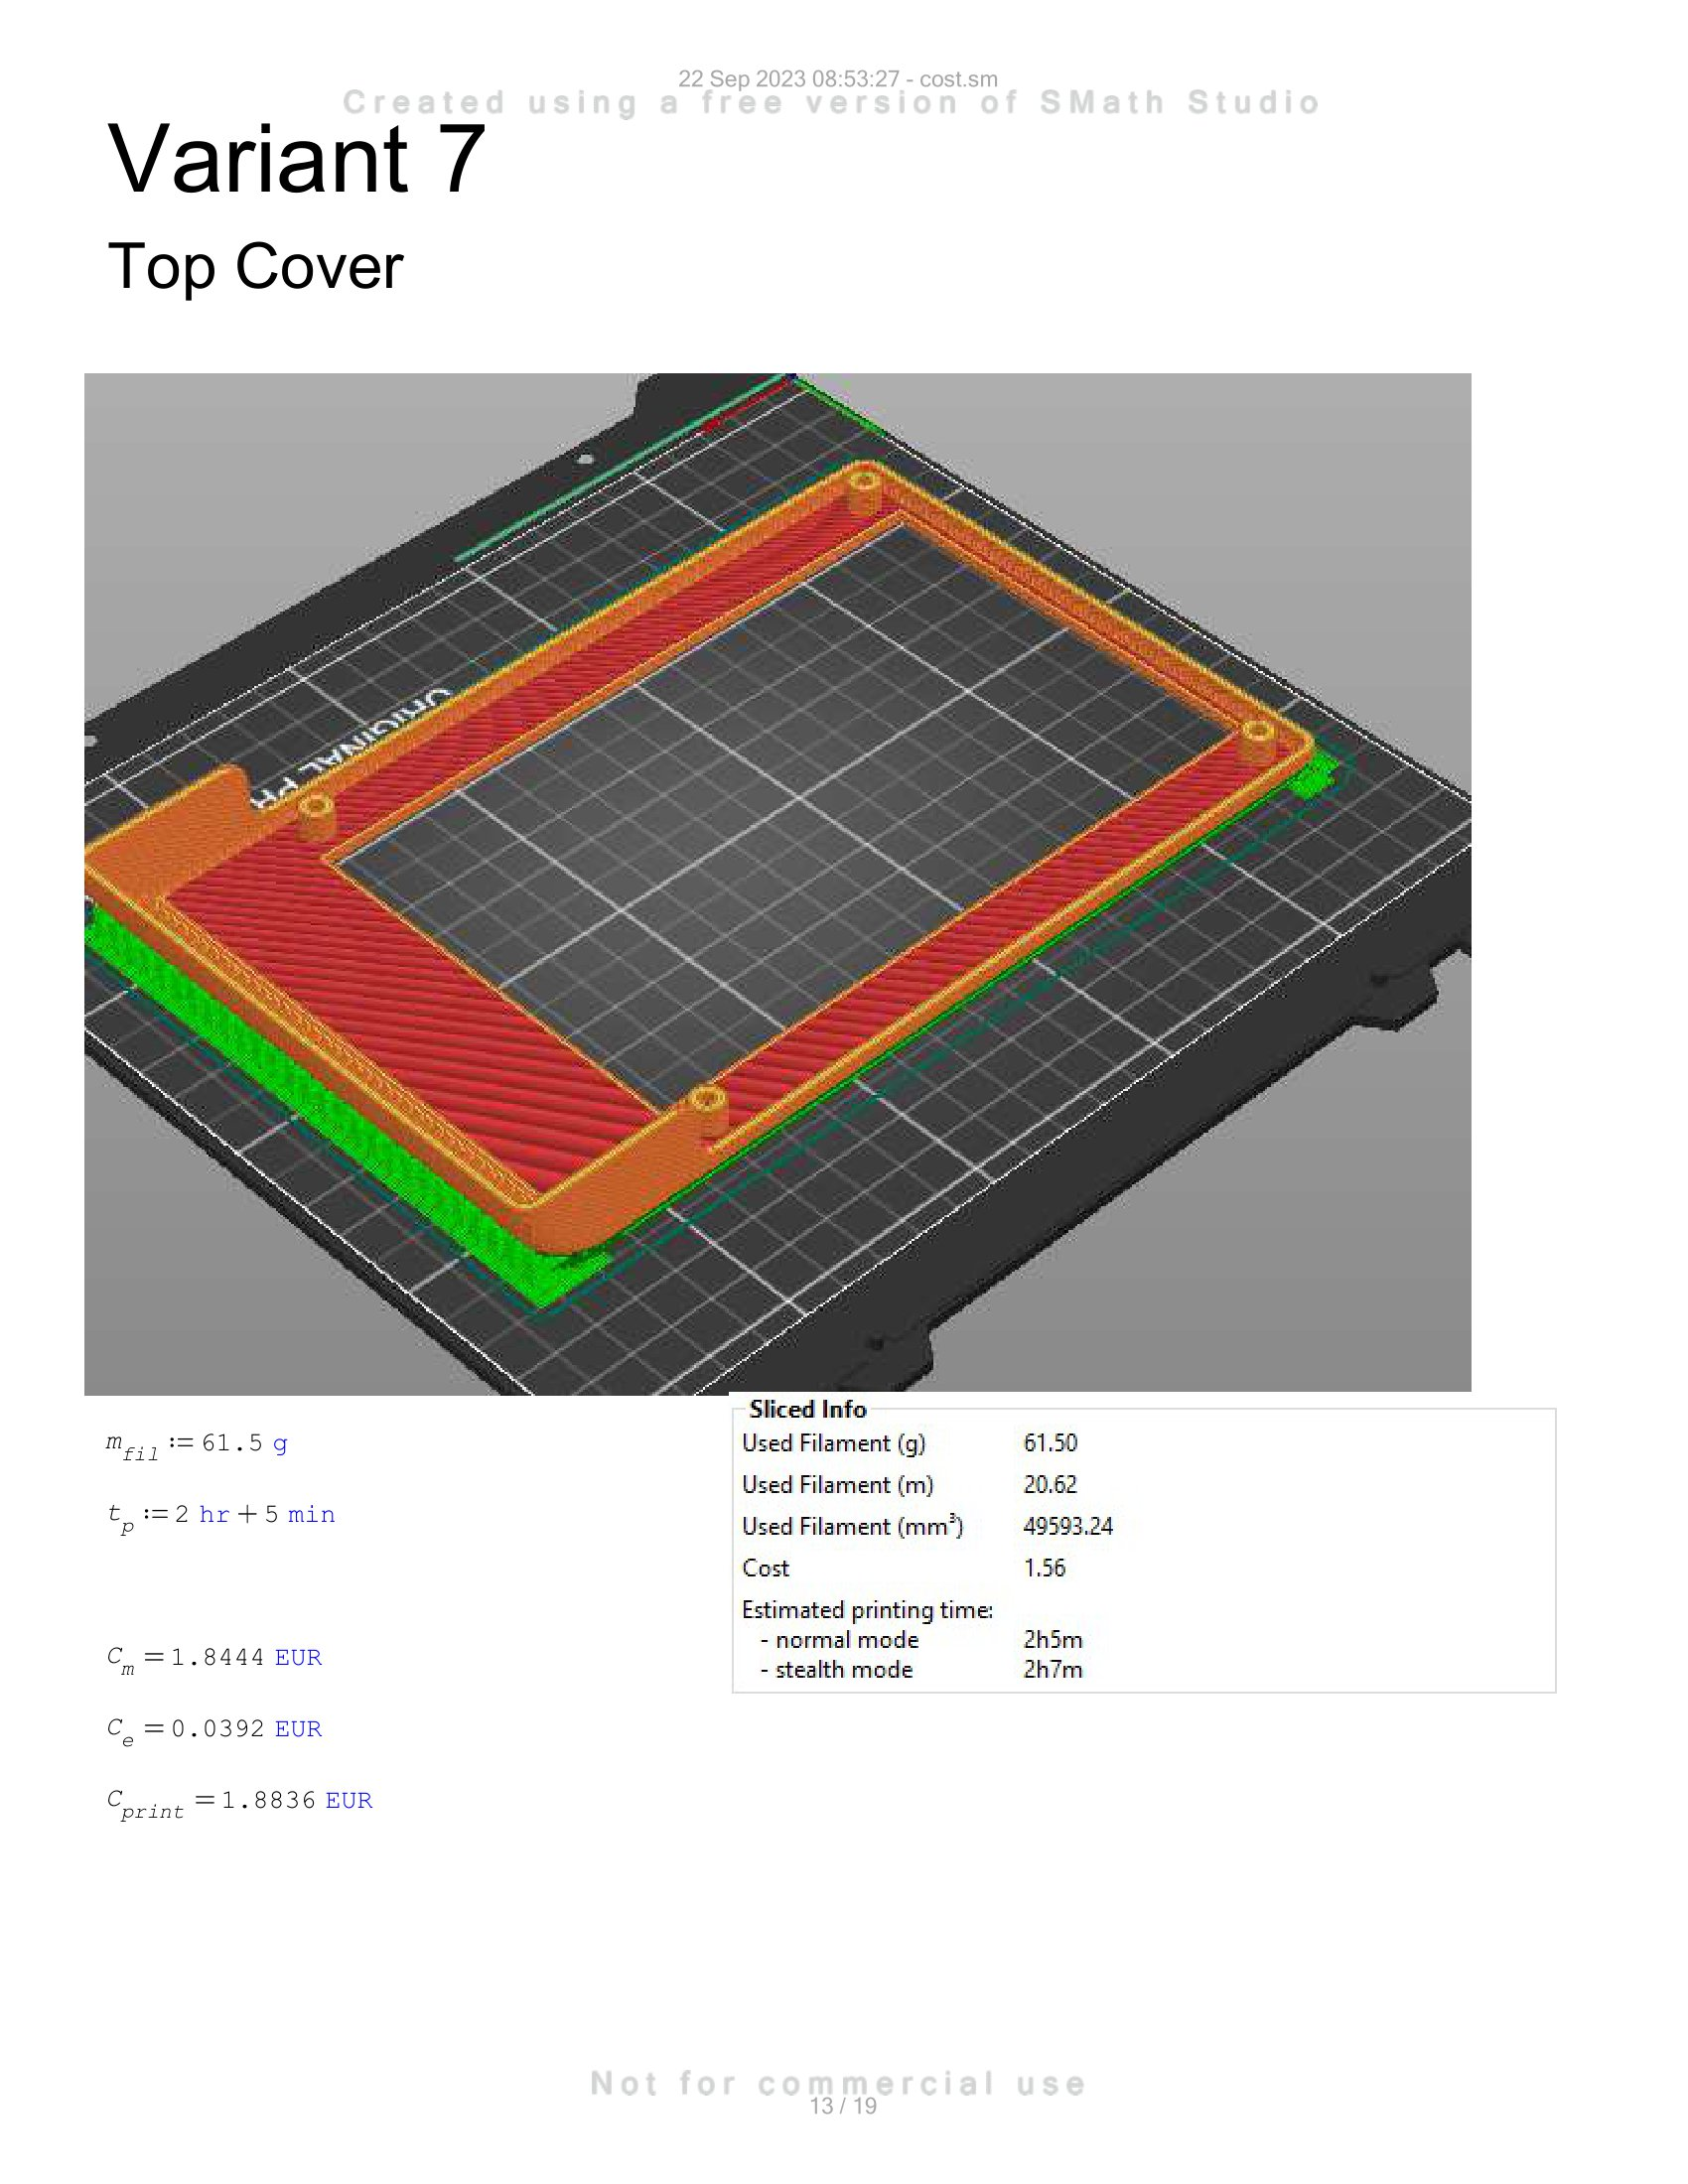
\includegraphics[width=\linewidth]{texs/appendix/data/costcalculation/cost1-13.jpg}
    \caption{Cost Calculation 13}
    \label{fig:cost-calculation-13}
\end{figure}

\begin{figure}[H]
    \centering
    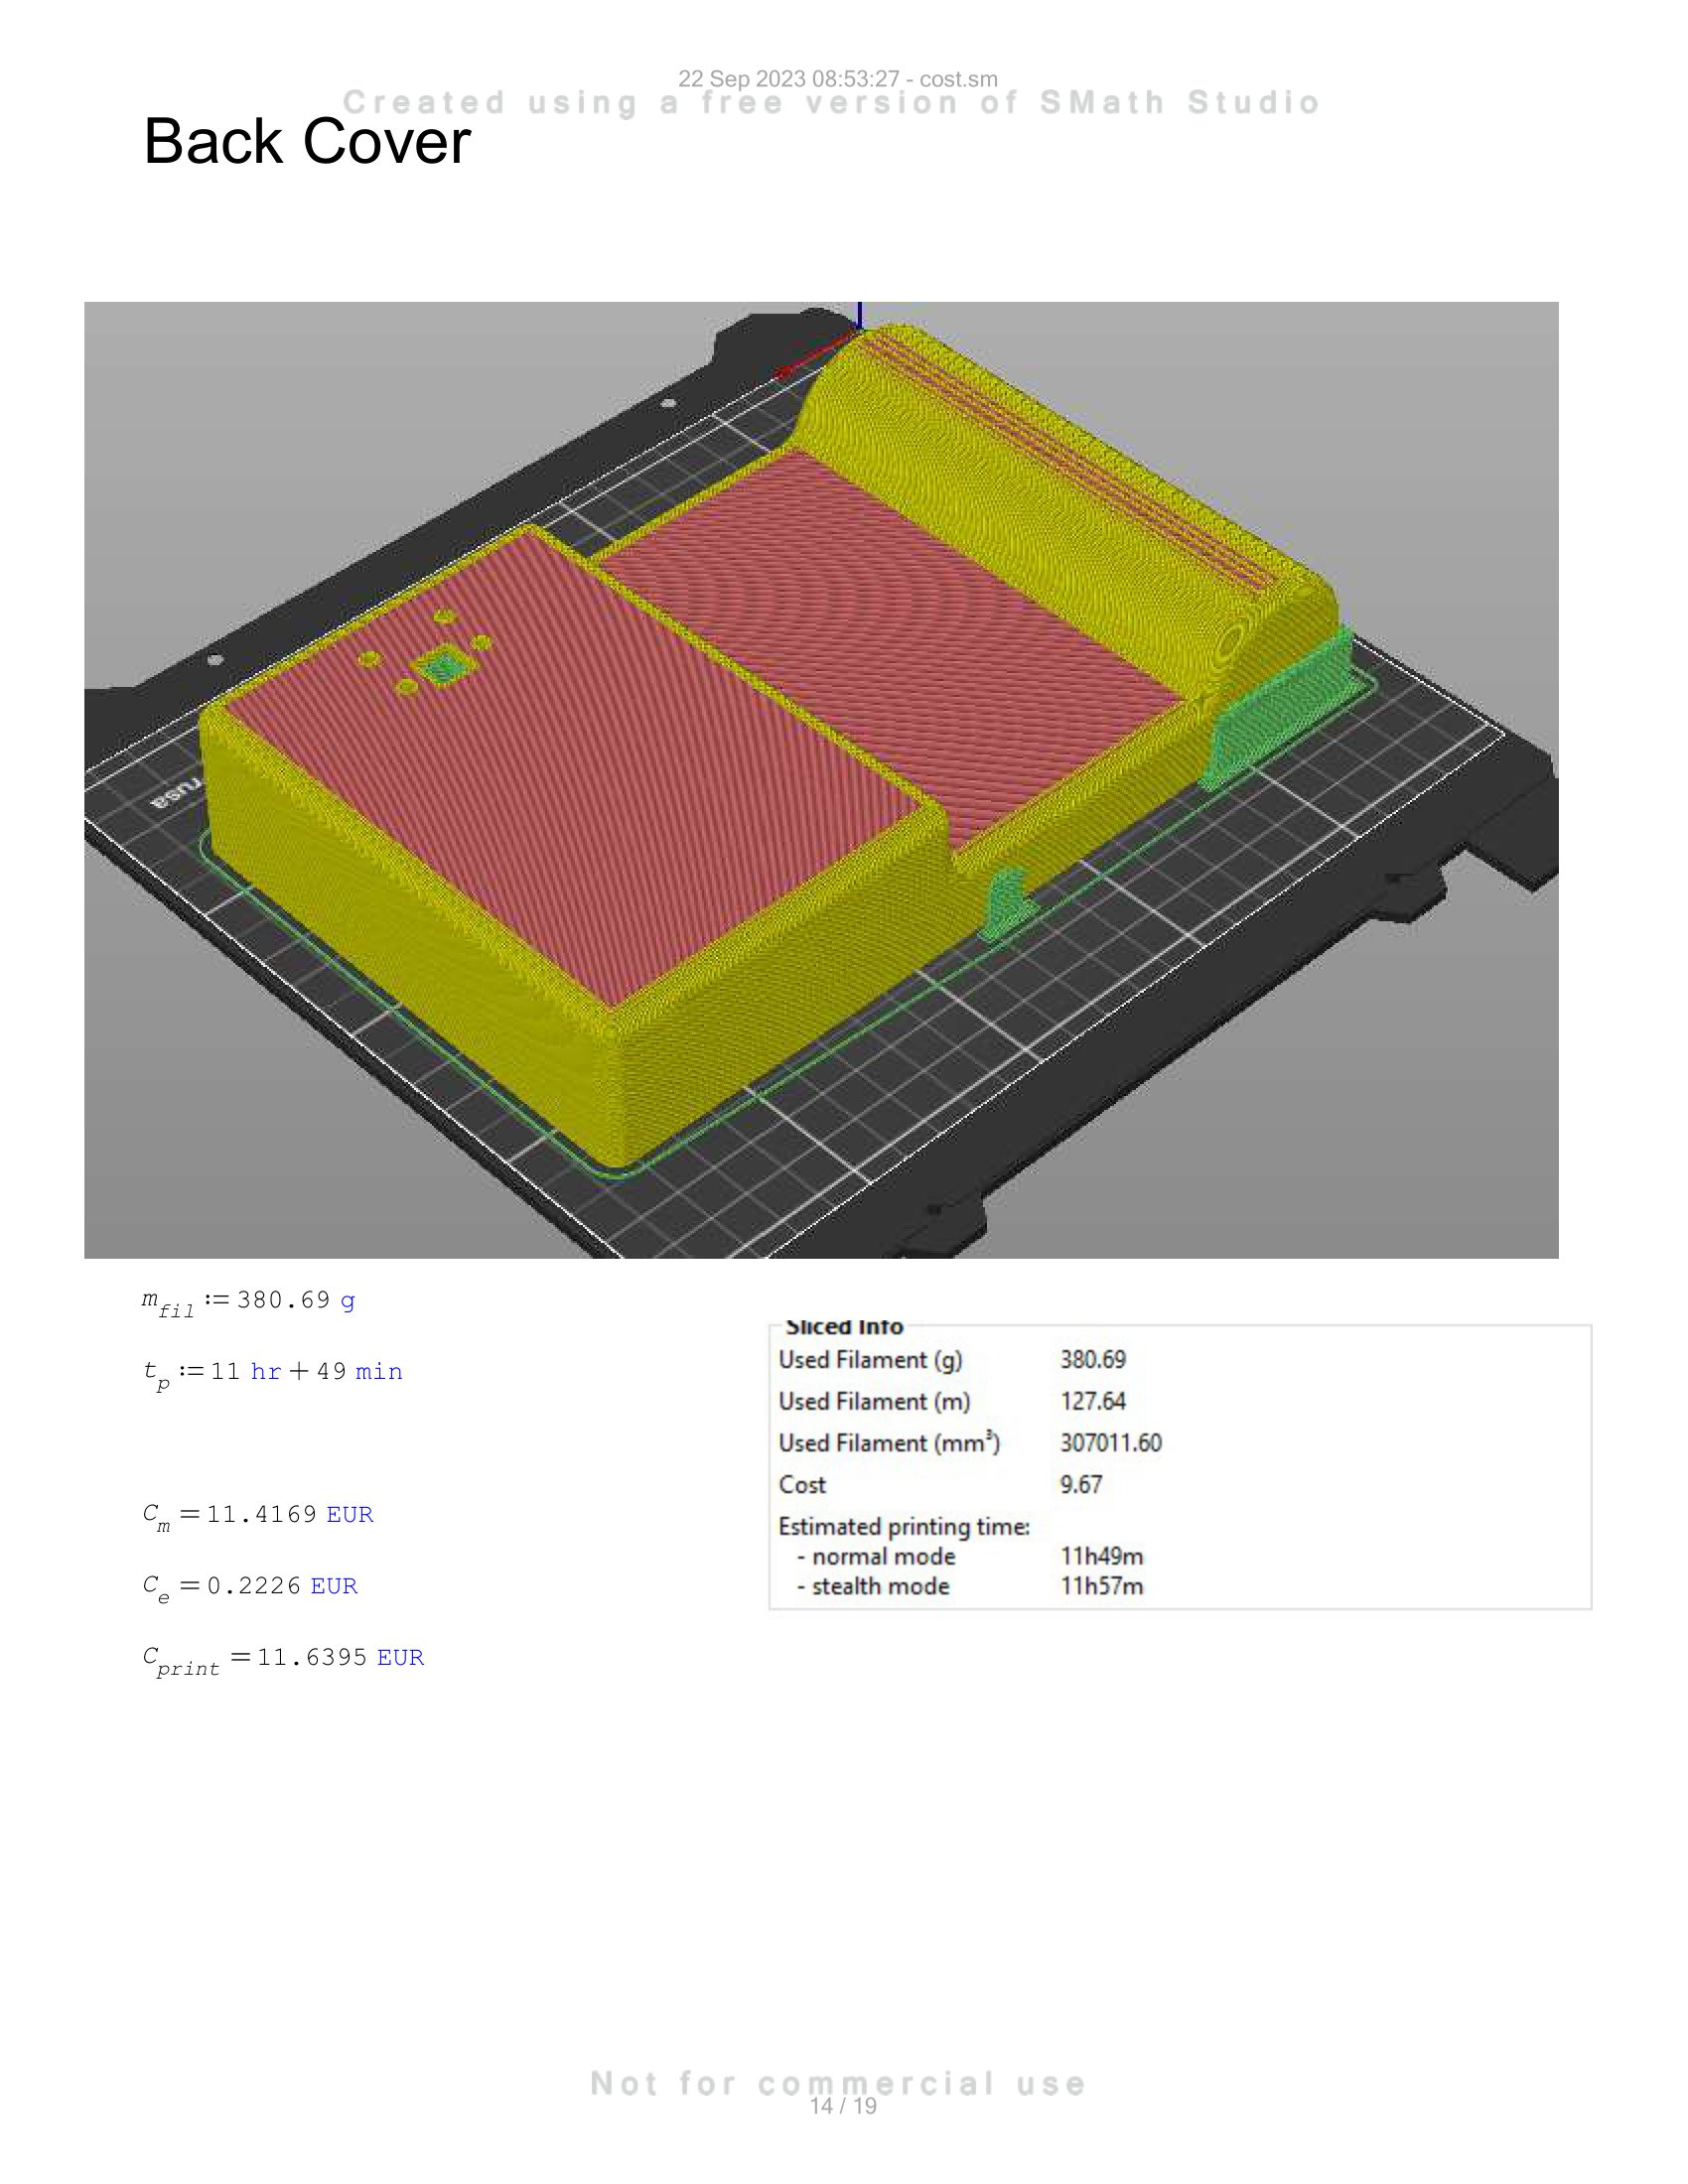
\includegraphics[width=\linewidth]{texs/appendix/data/costcalculation/cost1-14.jpg}
    \caption{Cost Calculation 14}
    \label{fig:cost-calculation-14}
\end{figure}

\begin{figure}[H]
    \centering
    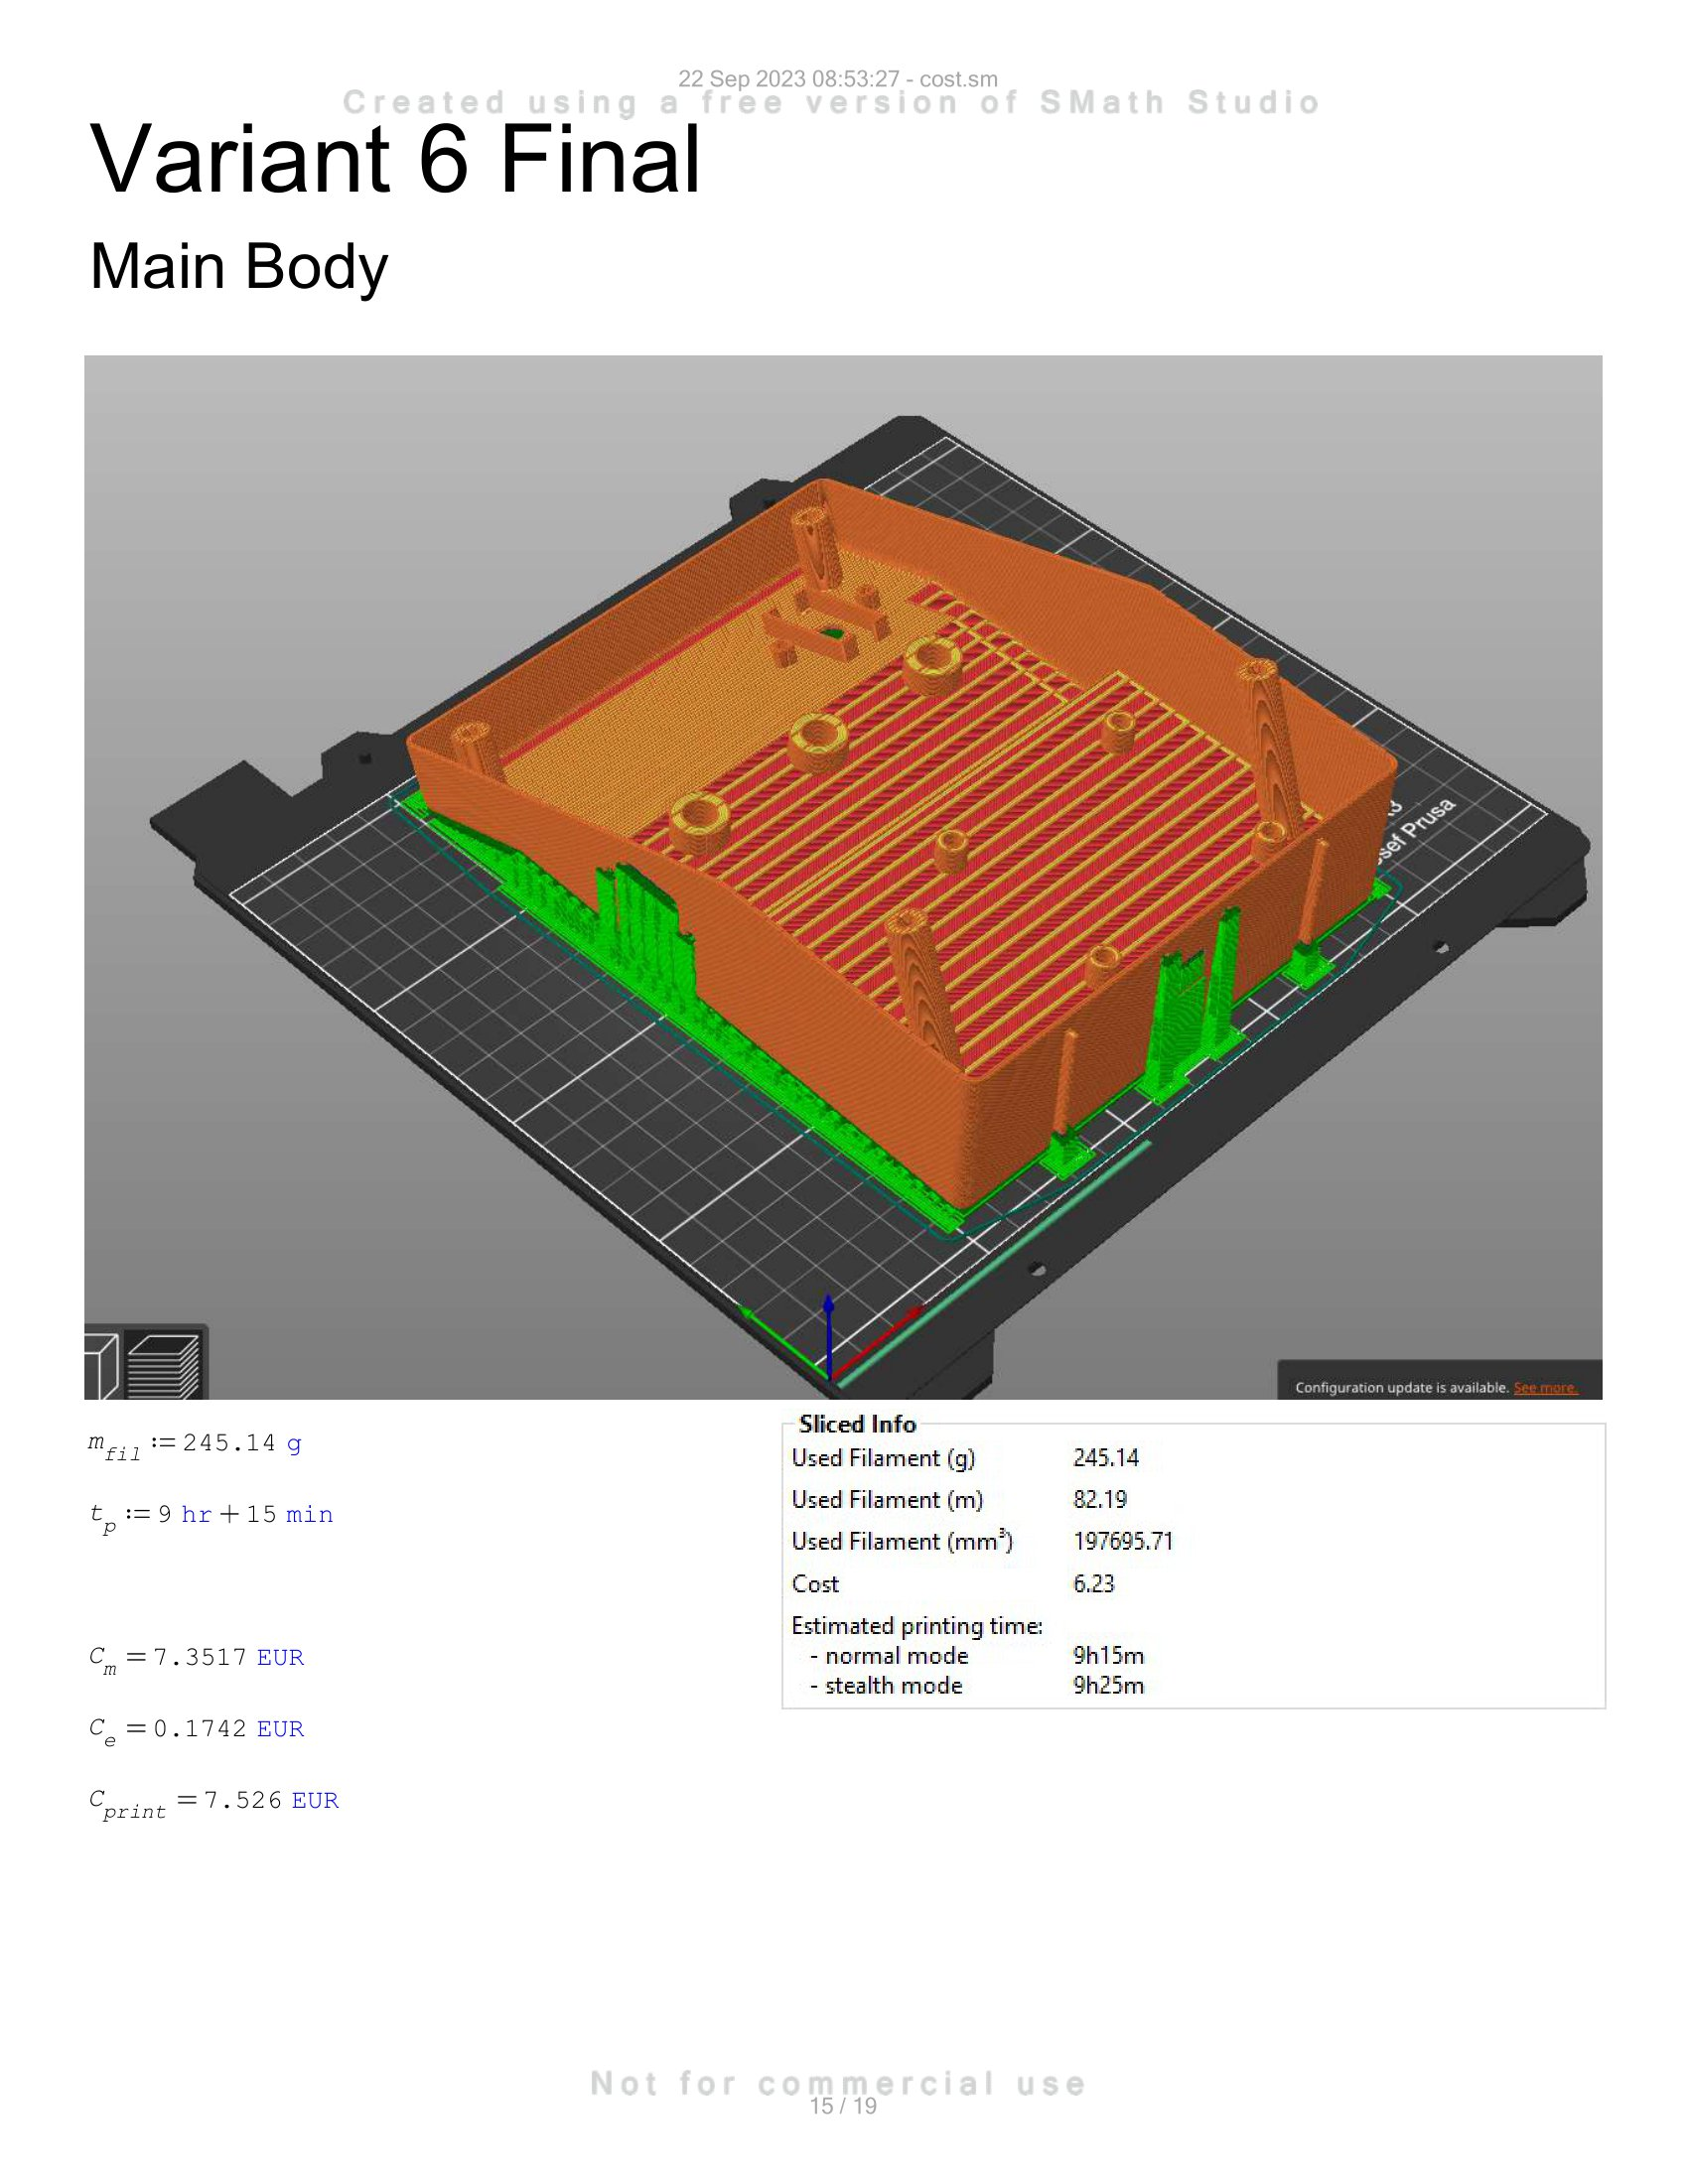
\includegraphics[width=\linewidth]{texs/appendix/data/costcalculation/cost1-15.jpg}
    \caption{Cost Calculation 15}
    \label{fig:cost-calculation-15}
\end{figure}

\begin{figure}[H]
    \centering
    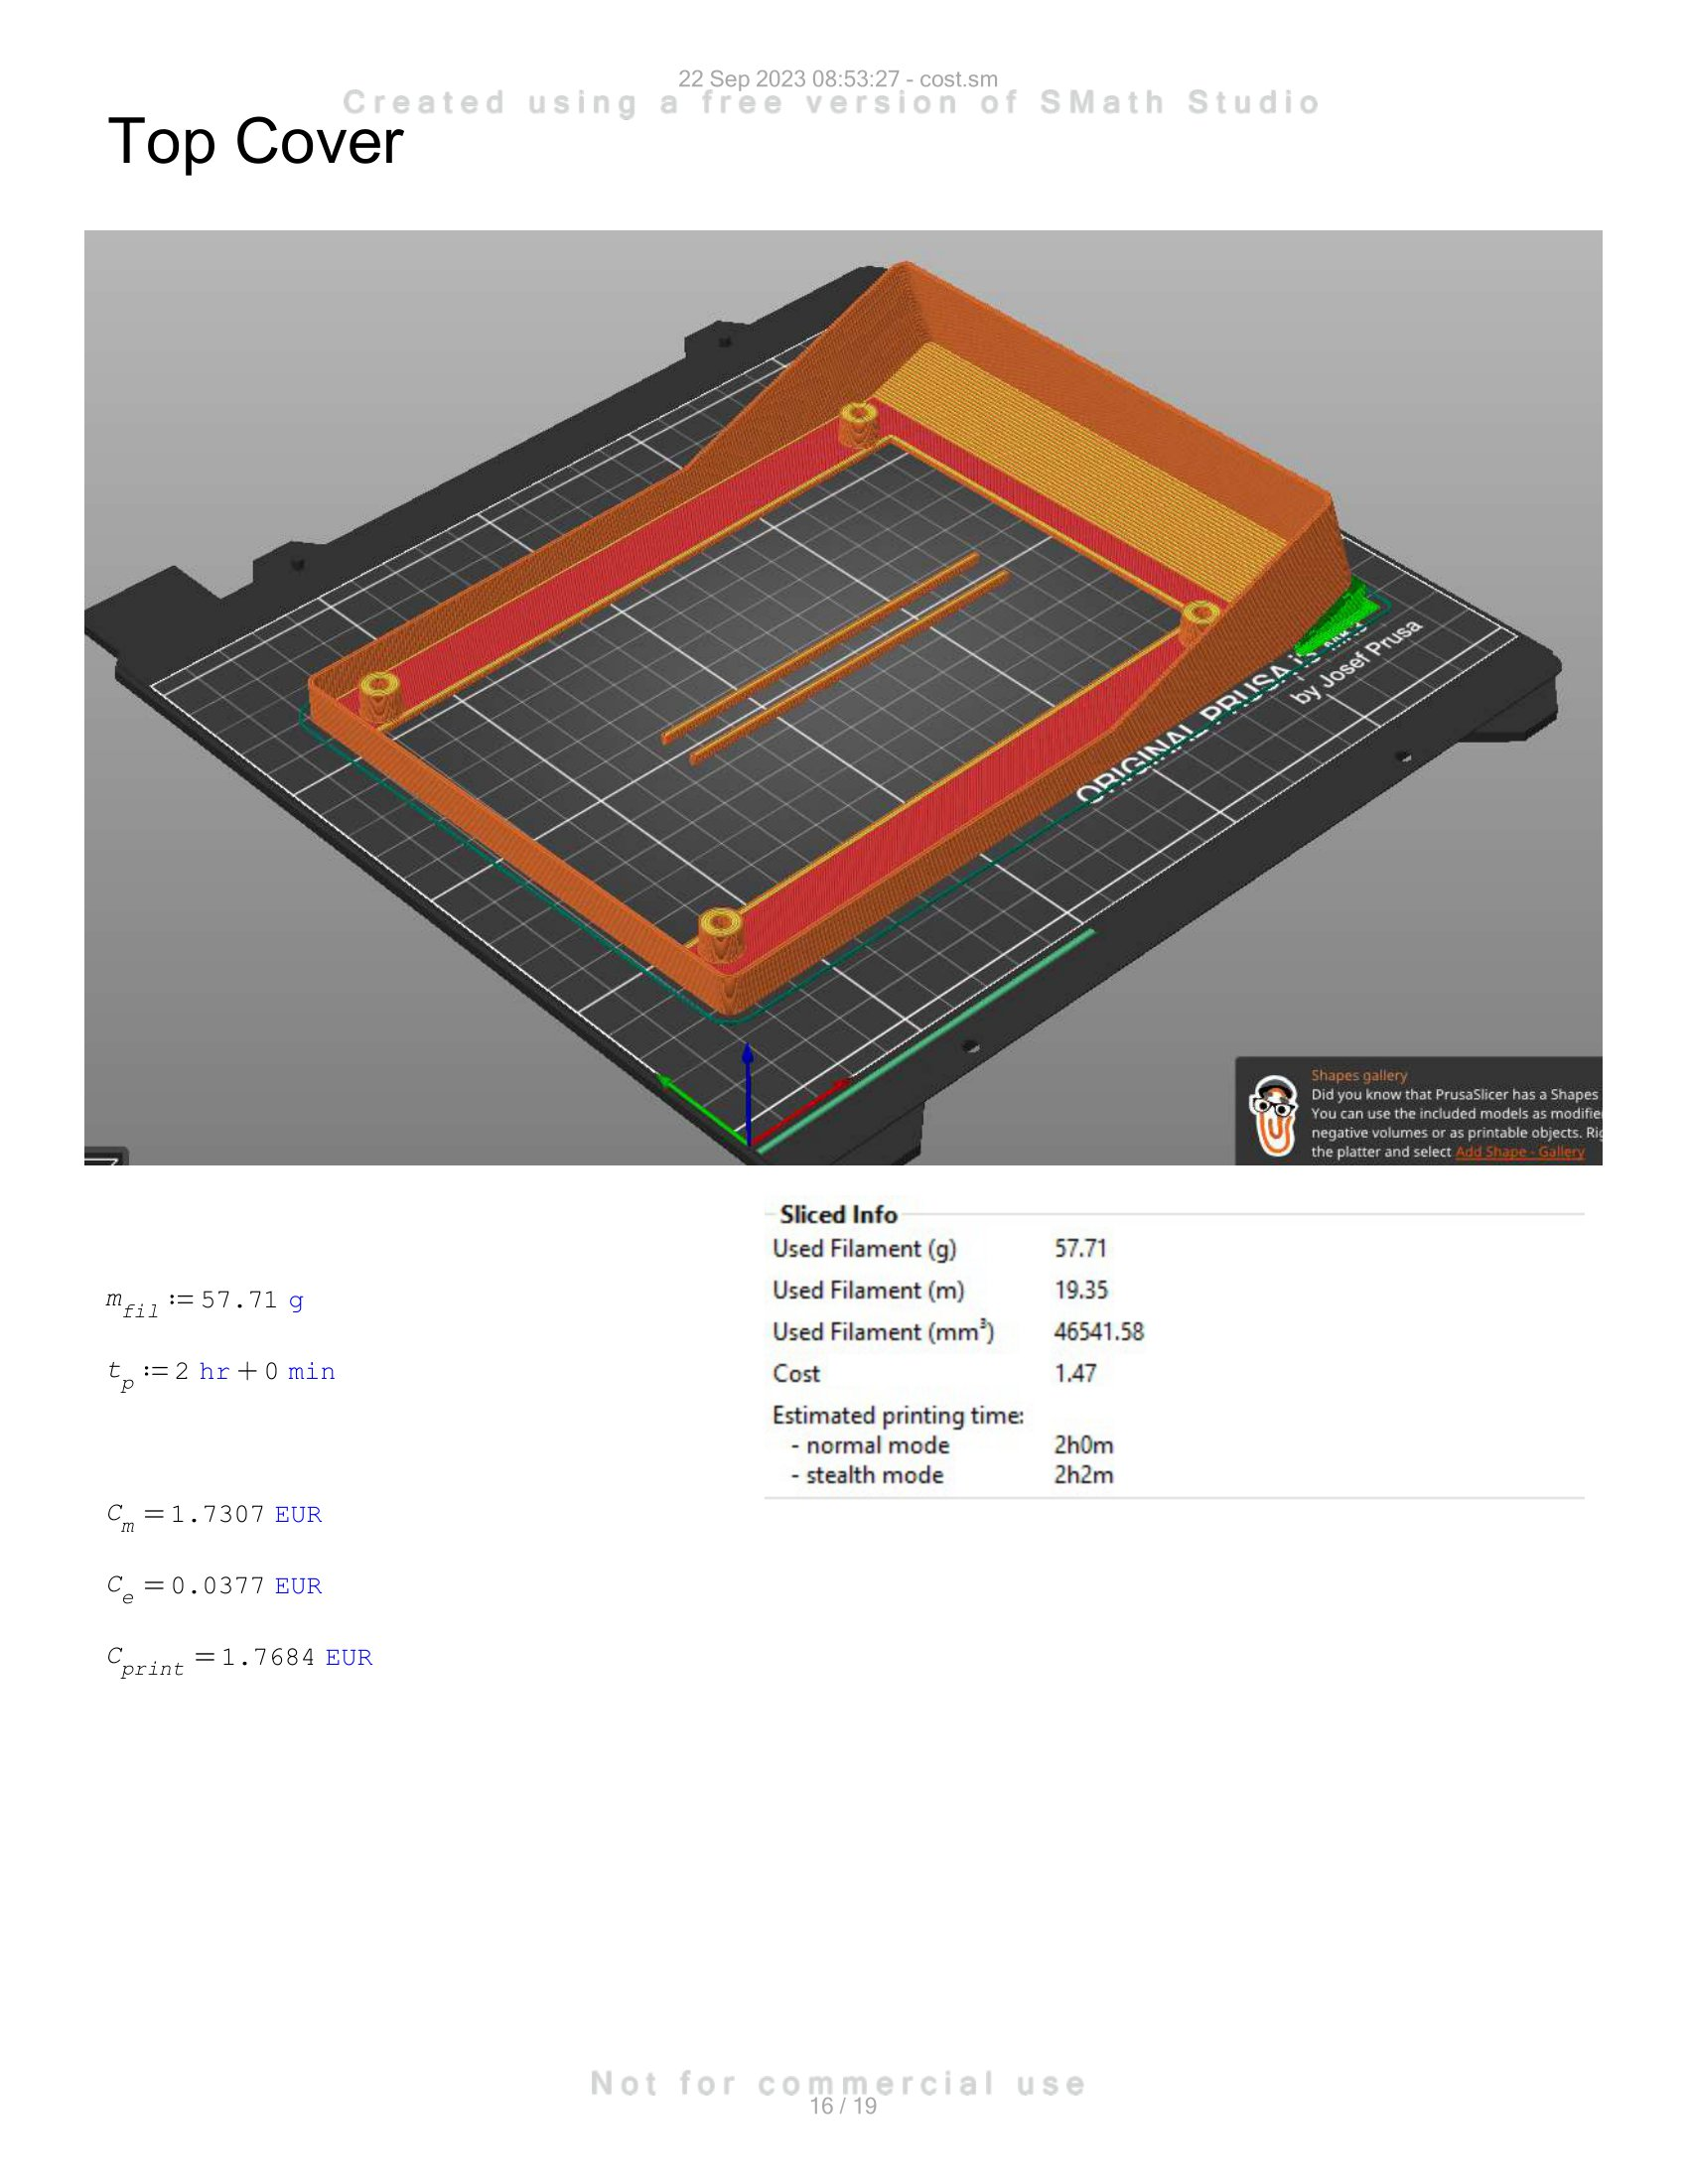
\includegraphics[width=\linewidth]{texs/appendix/data/costcalculation/cost1-16.jpg}
    \caption{Cost Calculation 16}
    \label{fig:cost-calculation-16}
\end{figure}

\begin{figure}[H]
    \centering
    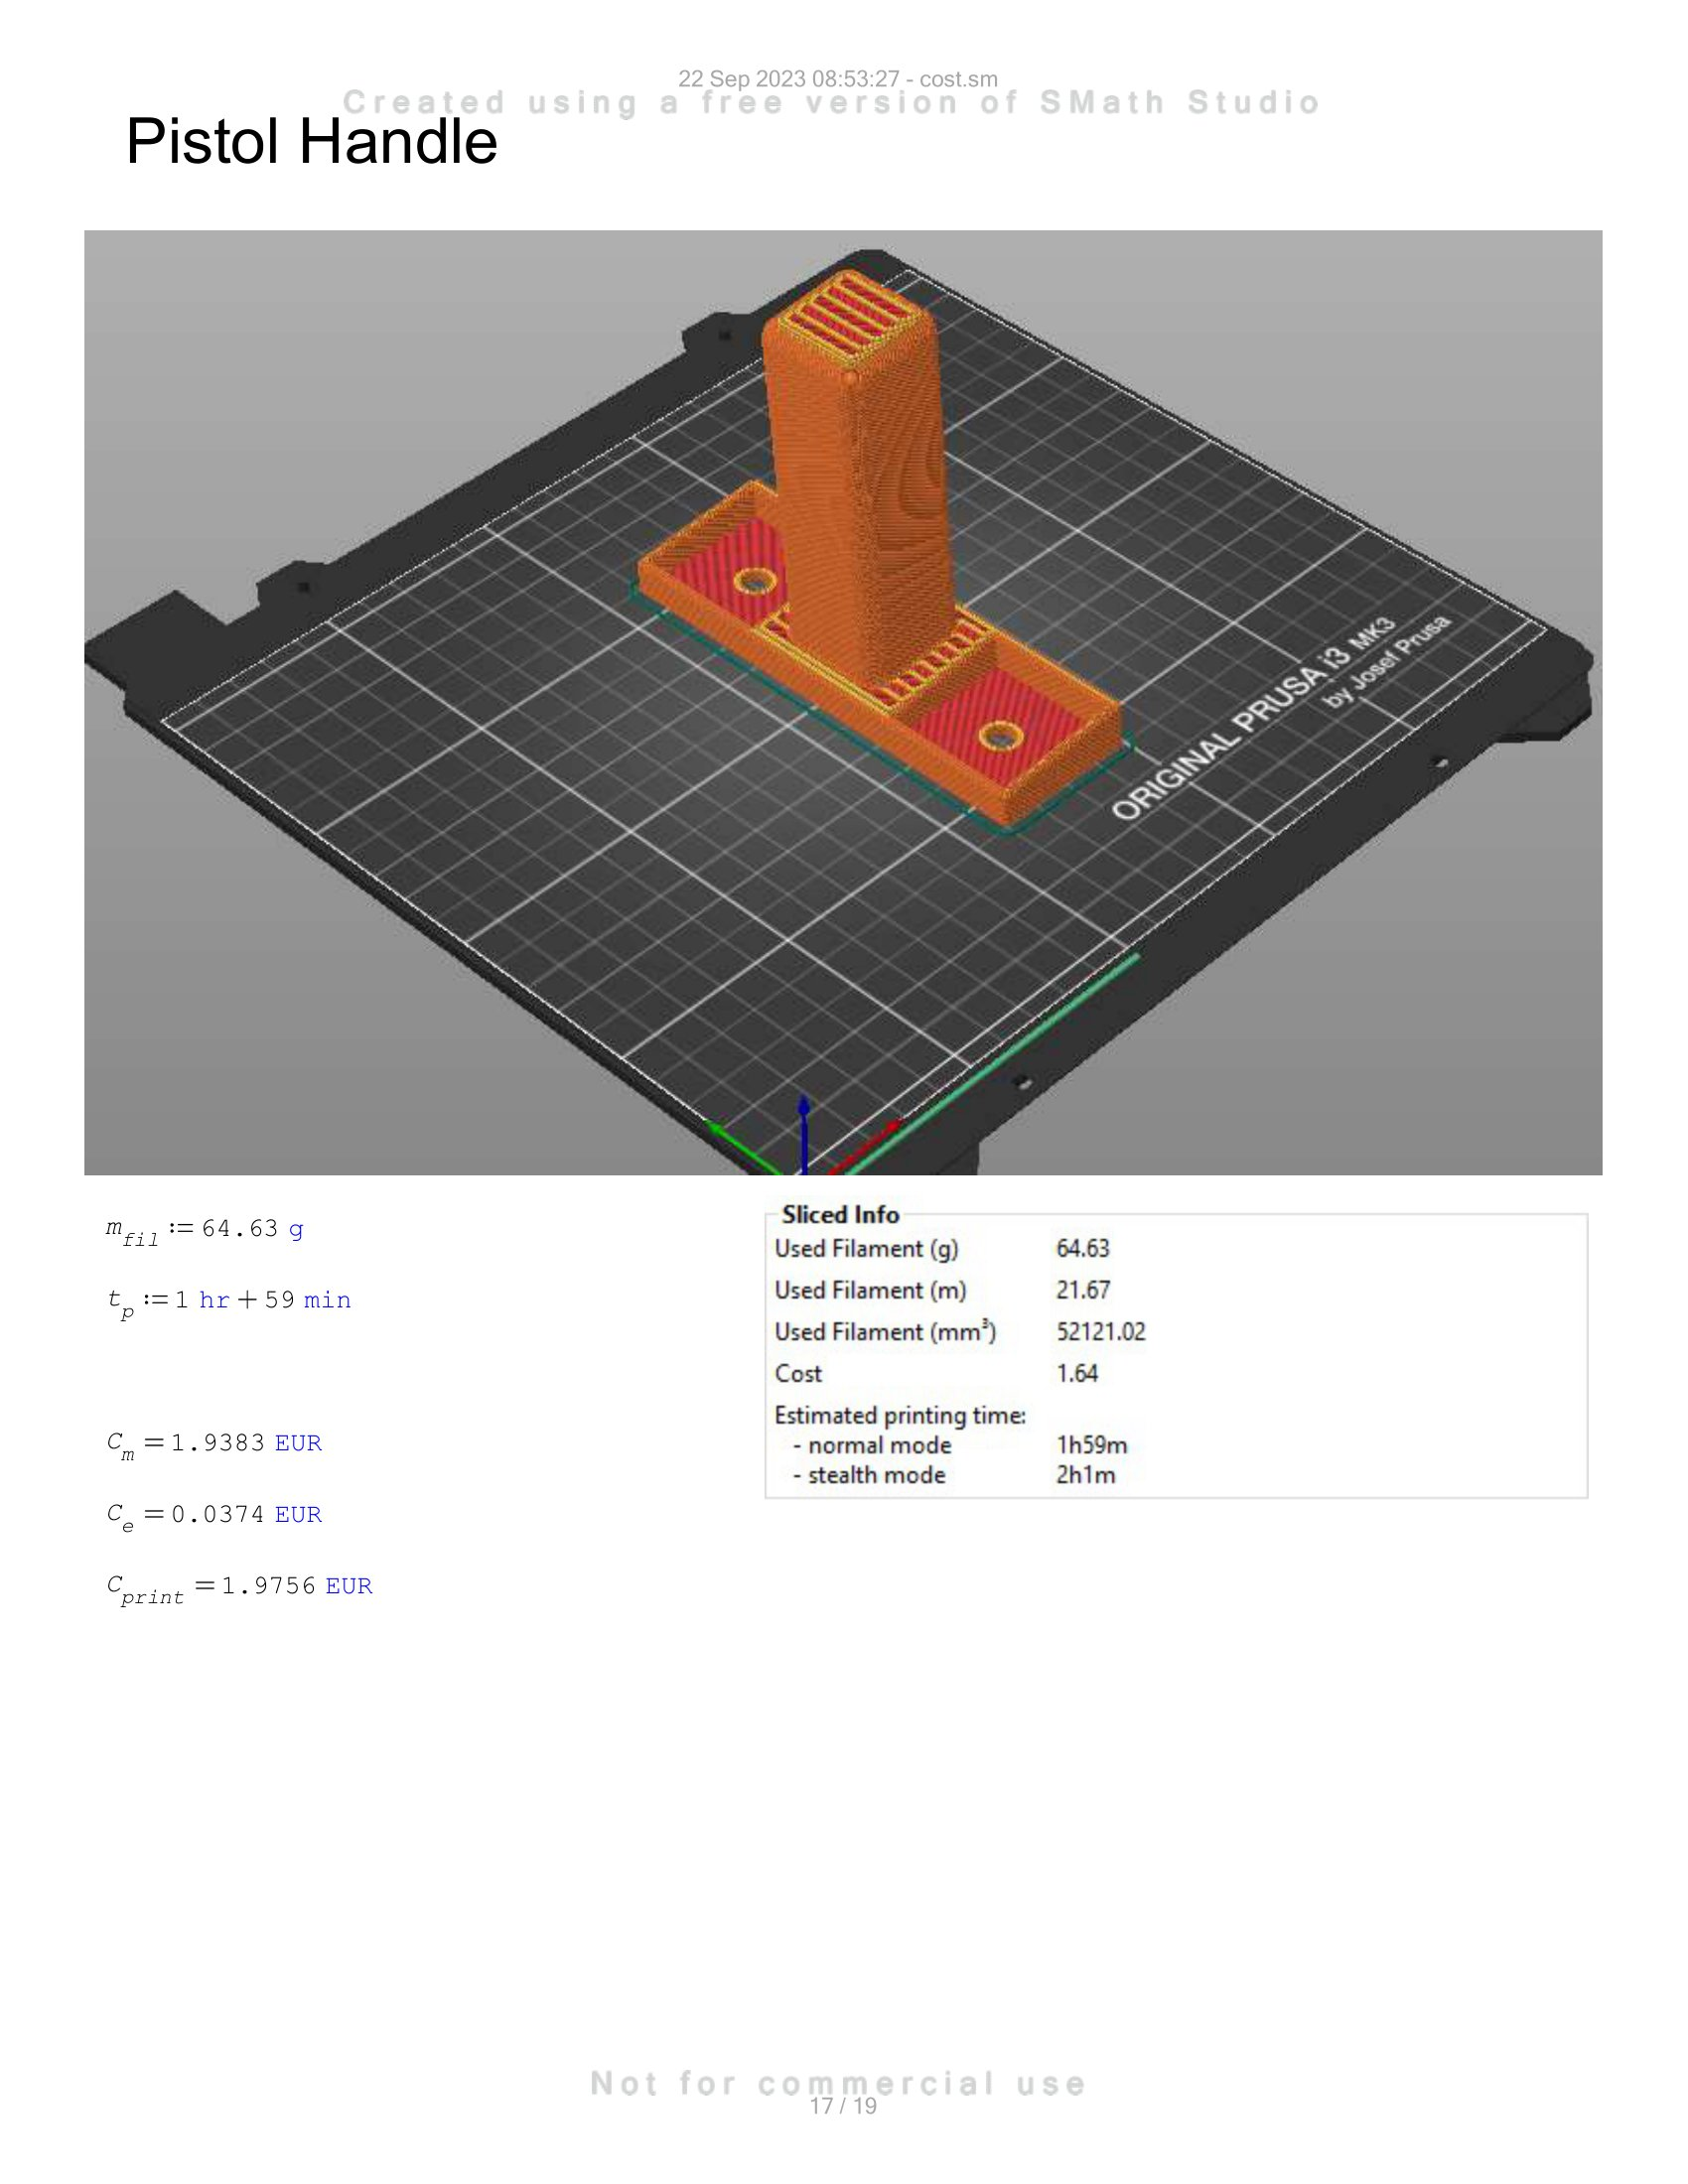
\includegraphics[width=\linewidth]{texs/appendix/data/costcalculation/cost1-17.jpg}
    \caption{Cost Calculation 17}
    \label{fig:cost-calculation-17}
\end{figure}

\begin{figure}[H]
    \centering
    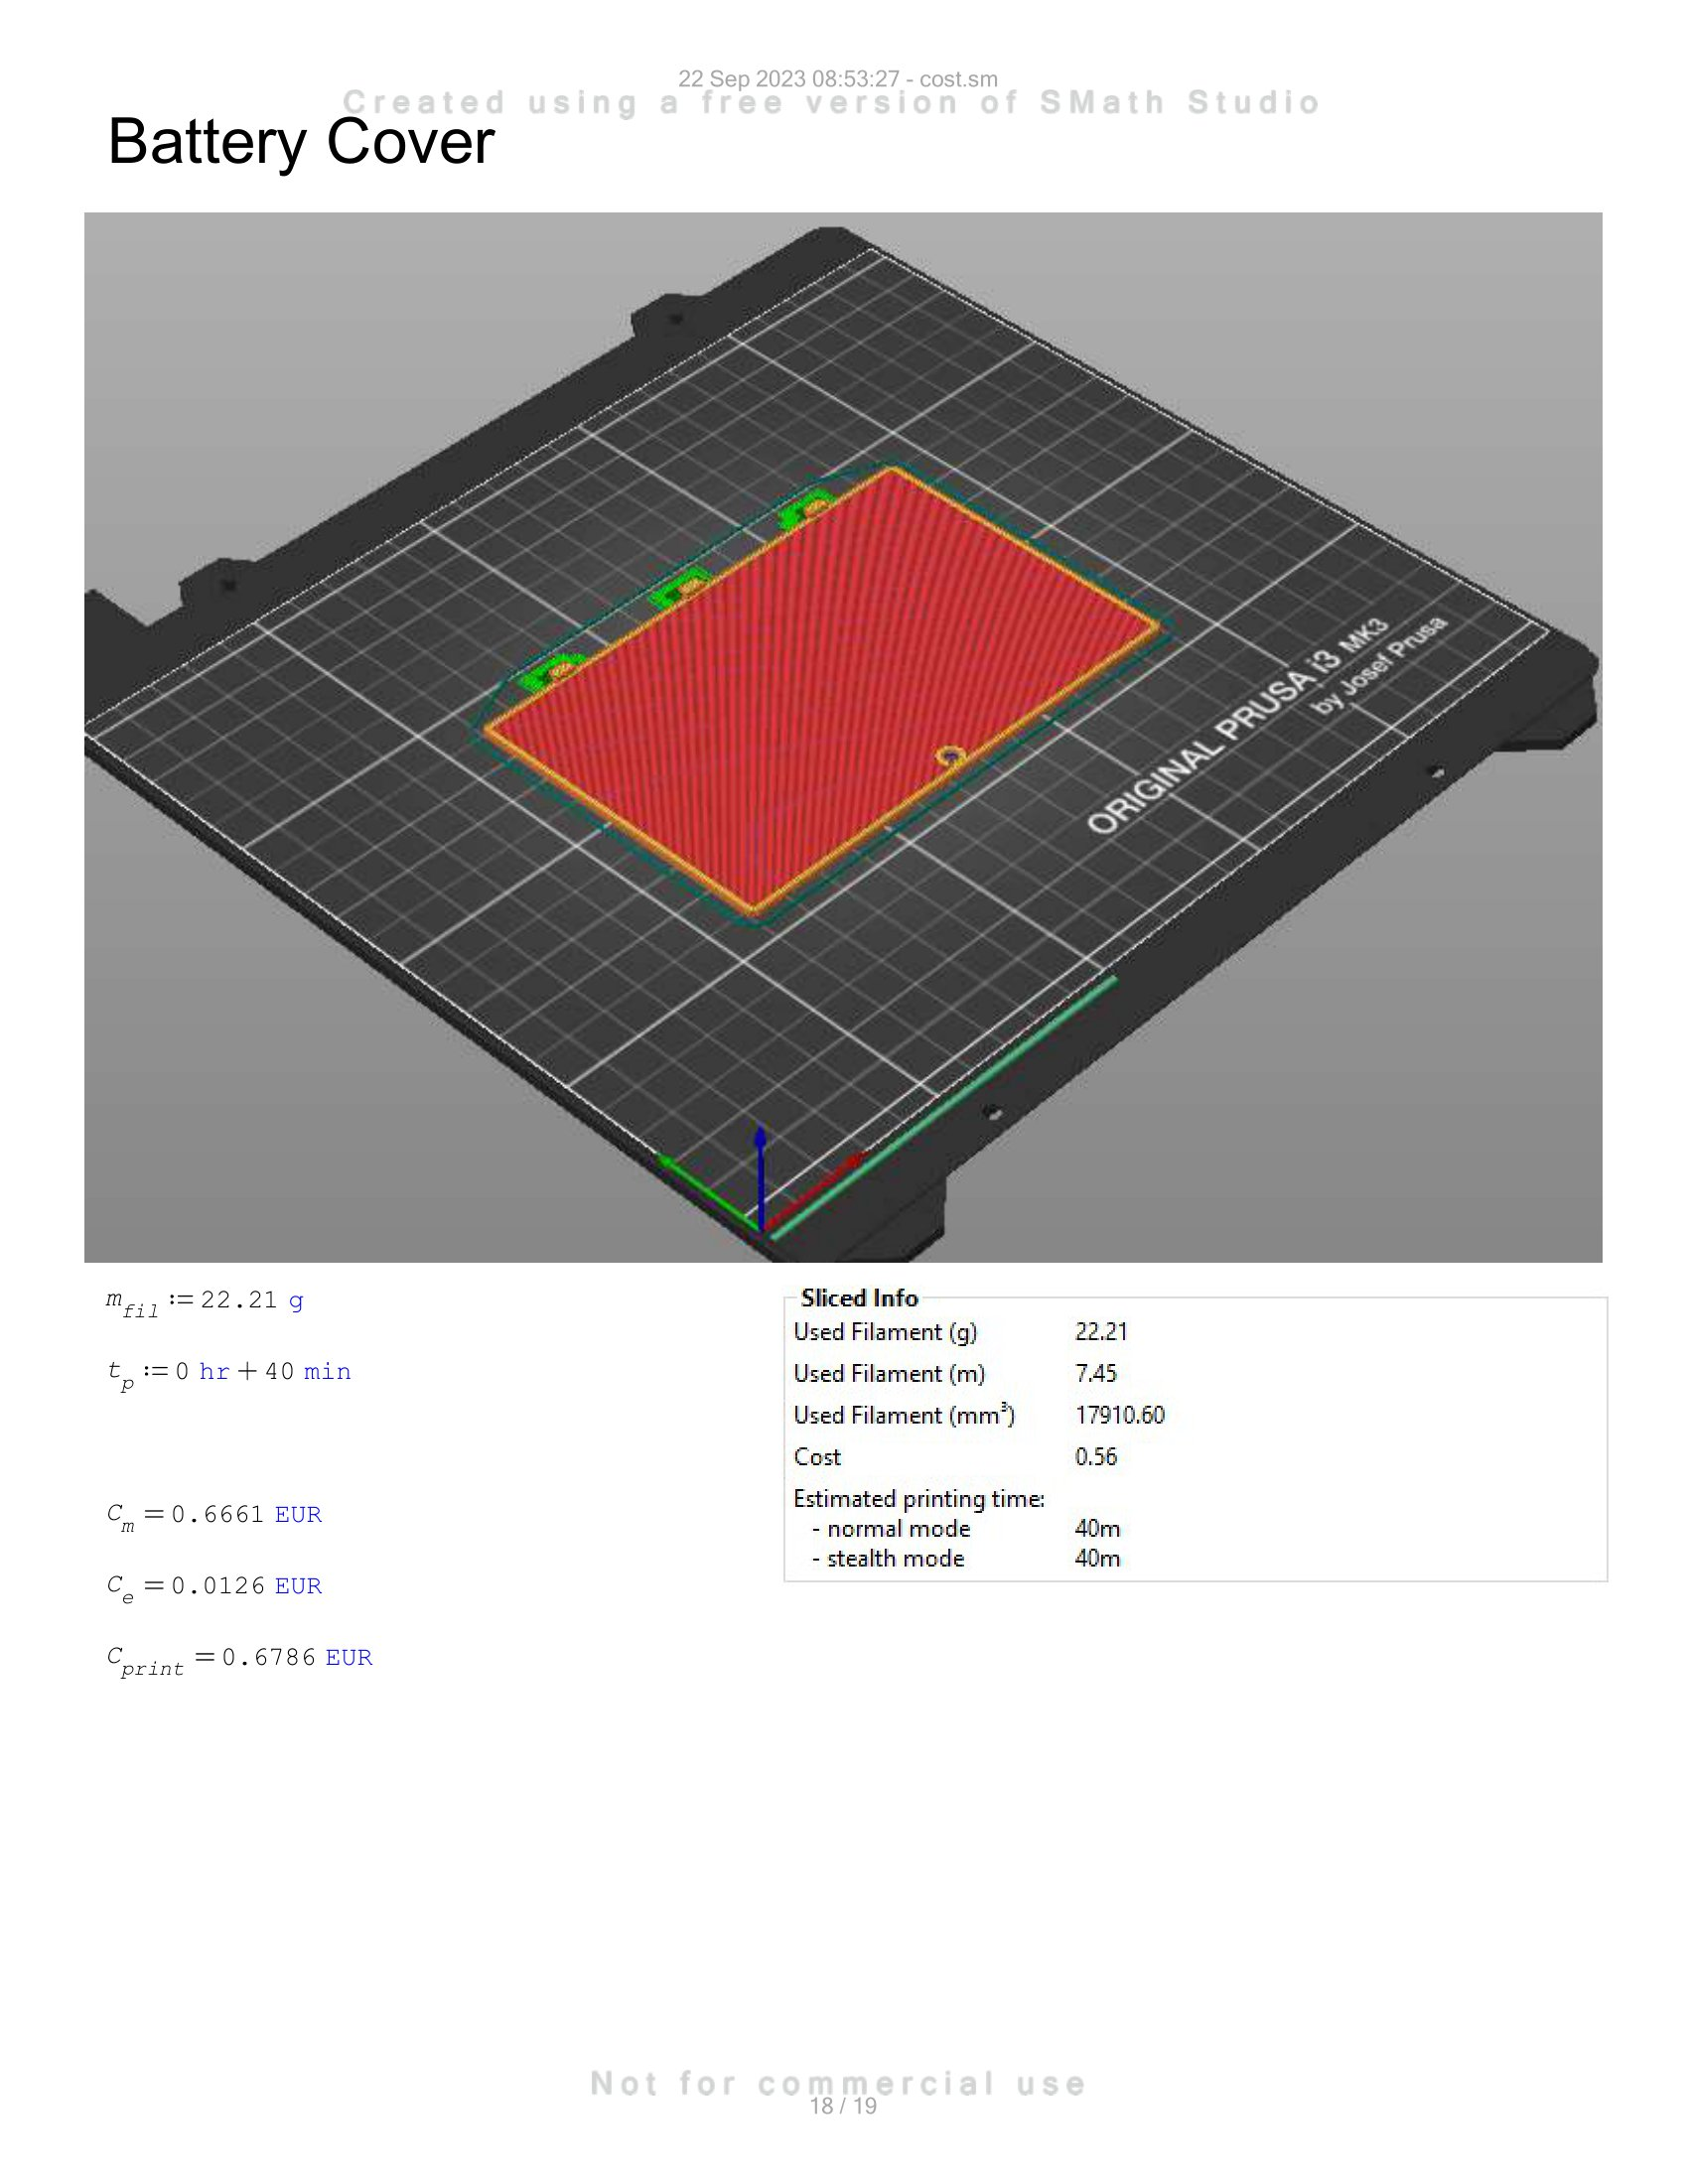
\includegraphics[width=\linewidth]{texs/appendix/data/costcalculation/cost1-18.jpg}
    \caption{Cost Calculation 18}
    \label{fig:cost-calculation-18}
\end{figure}

\begin{figure}[H]
    \centering
    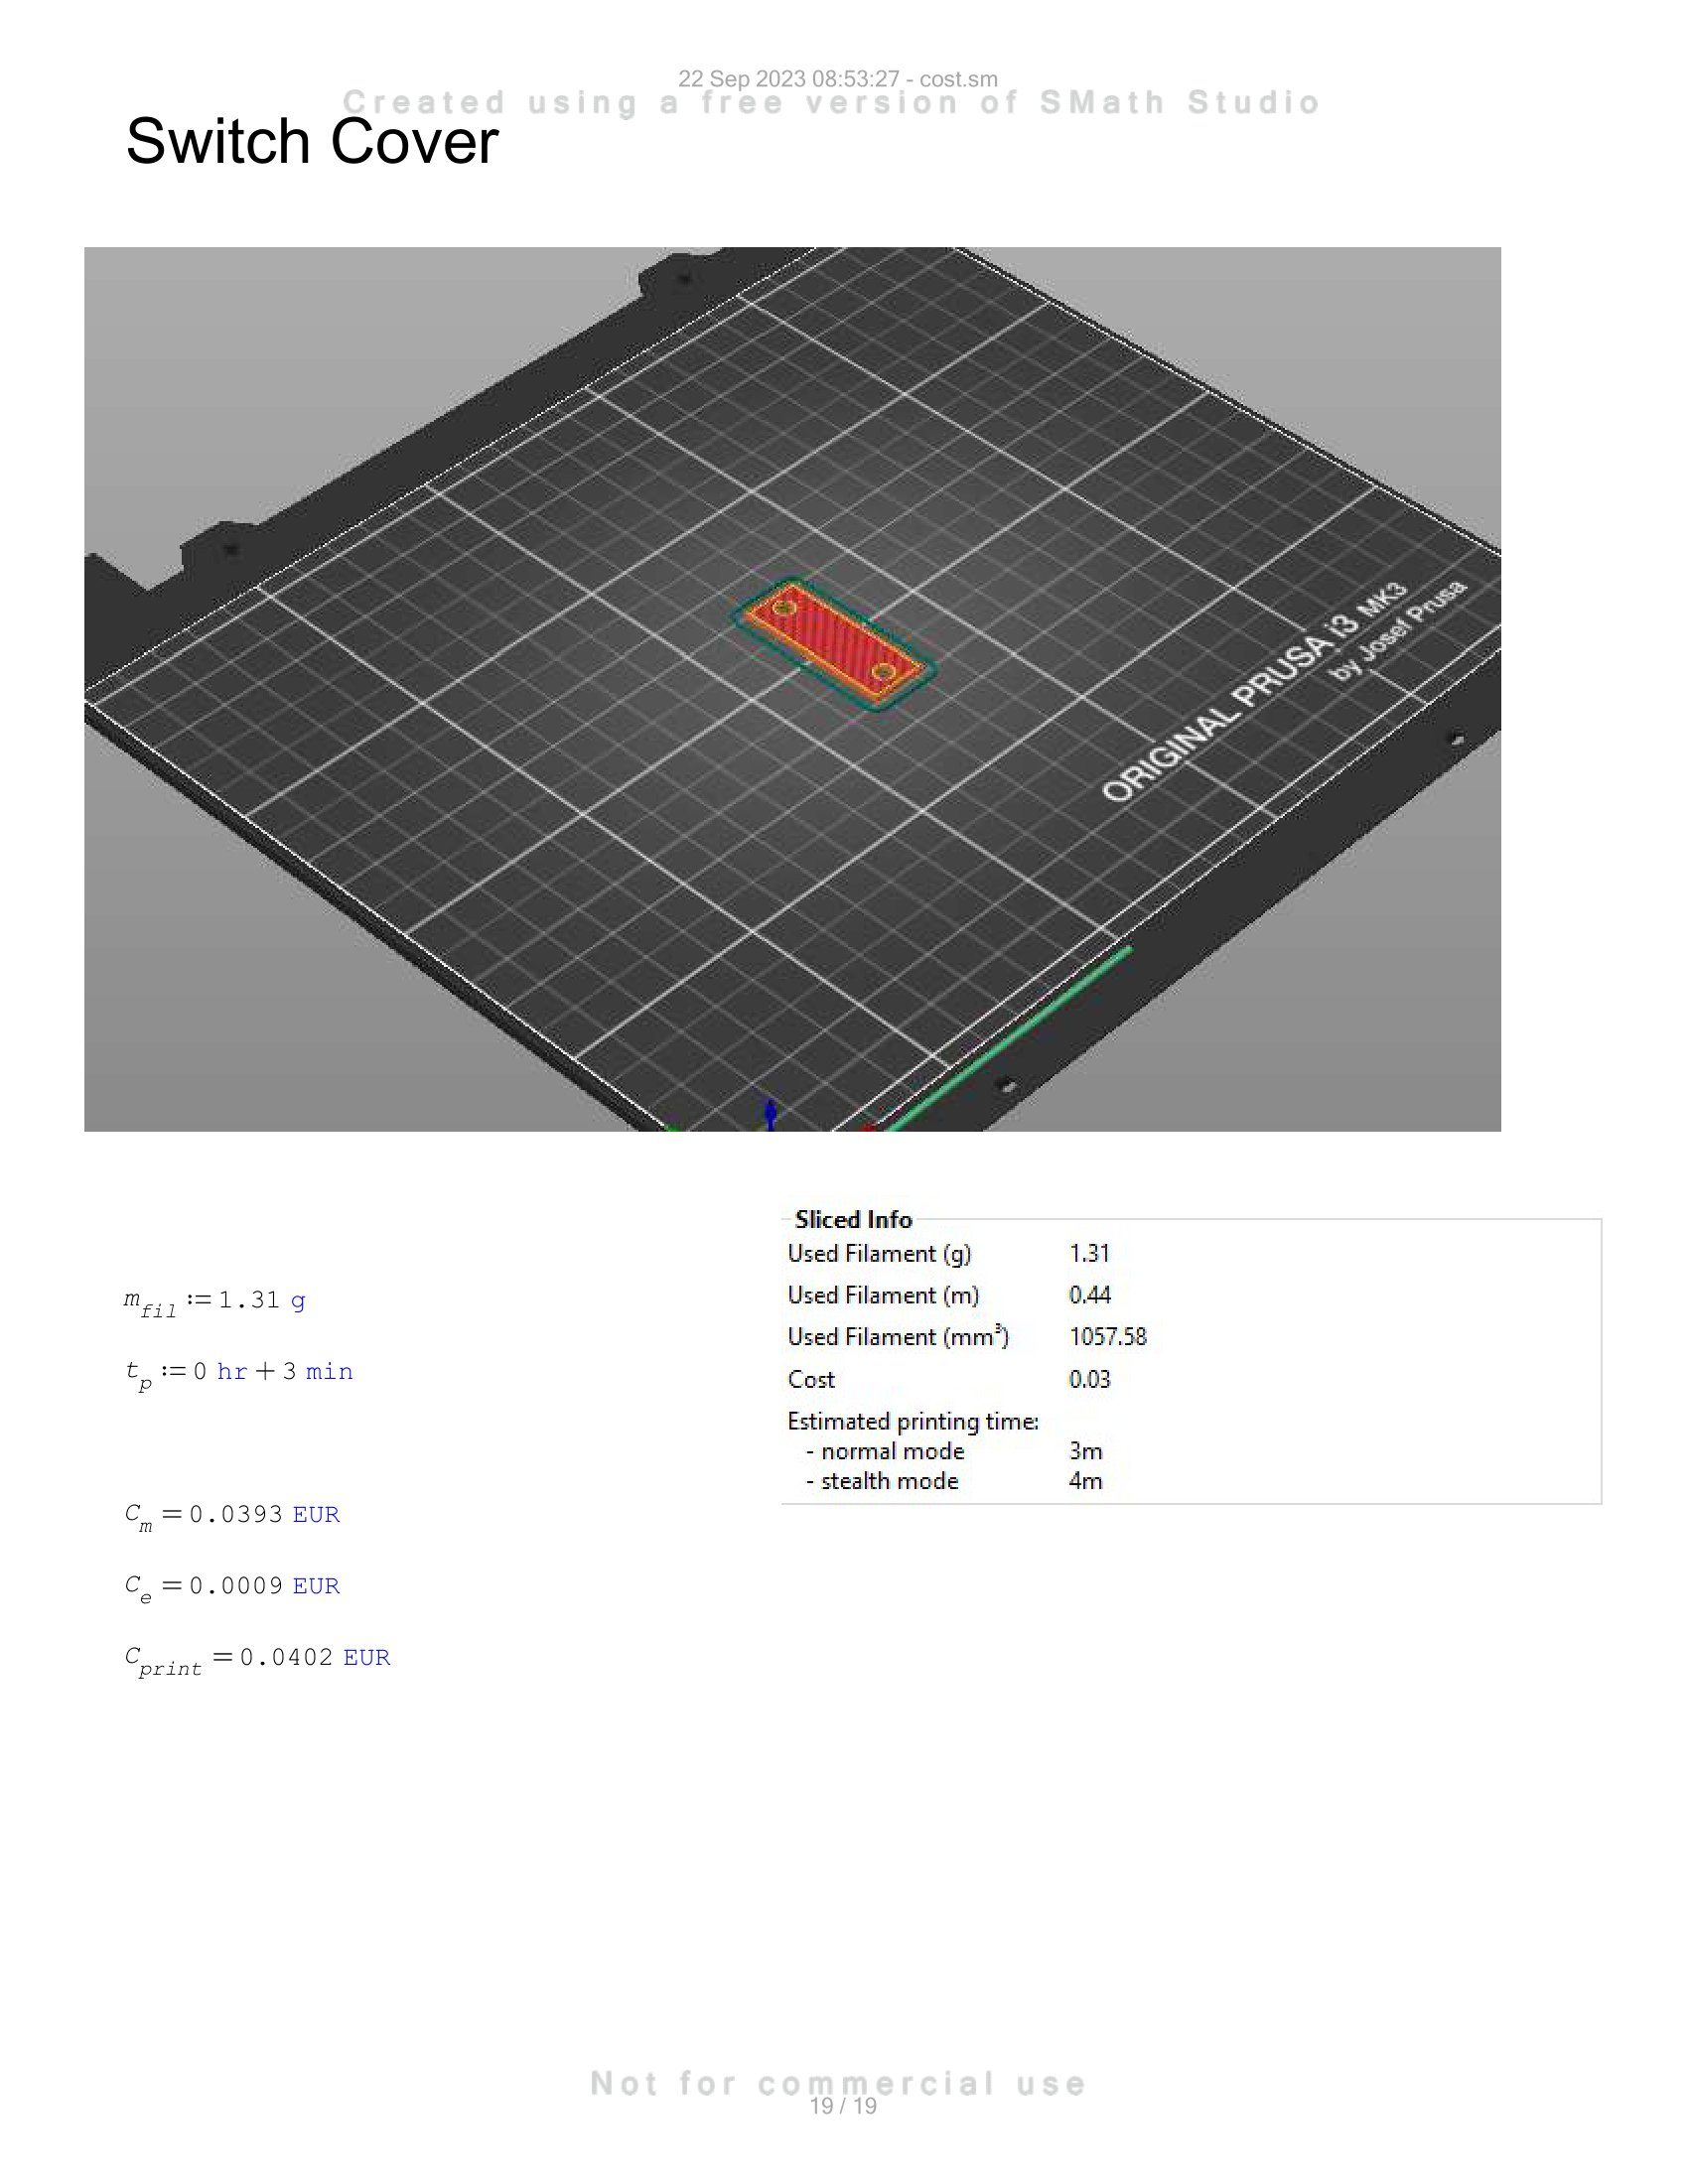
\includegraphics[width=\linewidth]{texs/appendix/data/costcalculation/cost1-19.jpg}
    \caption{Cost Calculation 19}
    \label{fig:cost-calculation-19}
\end{figure}

\section{Evaluation Data}
\label{appendix:evaluation-data}

\begin{figure}[H]
    \centering
    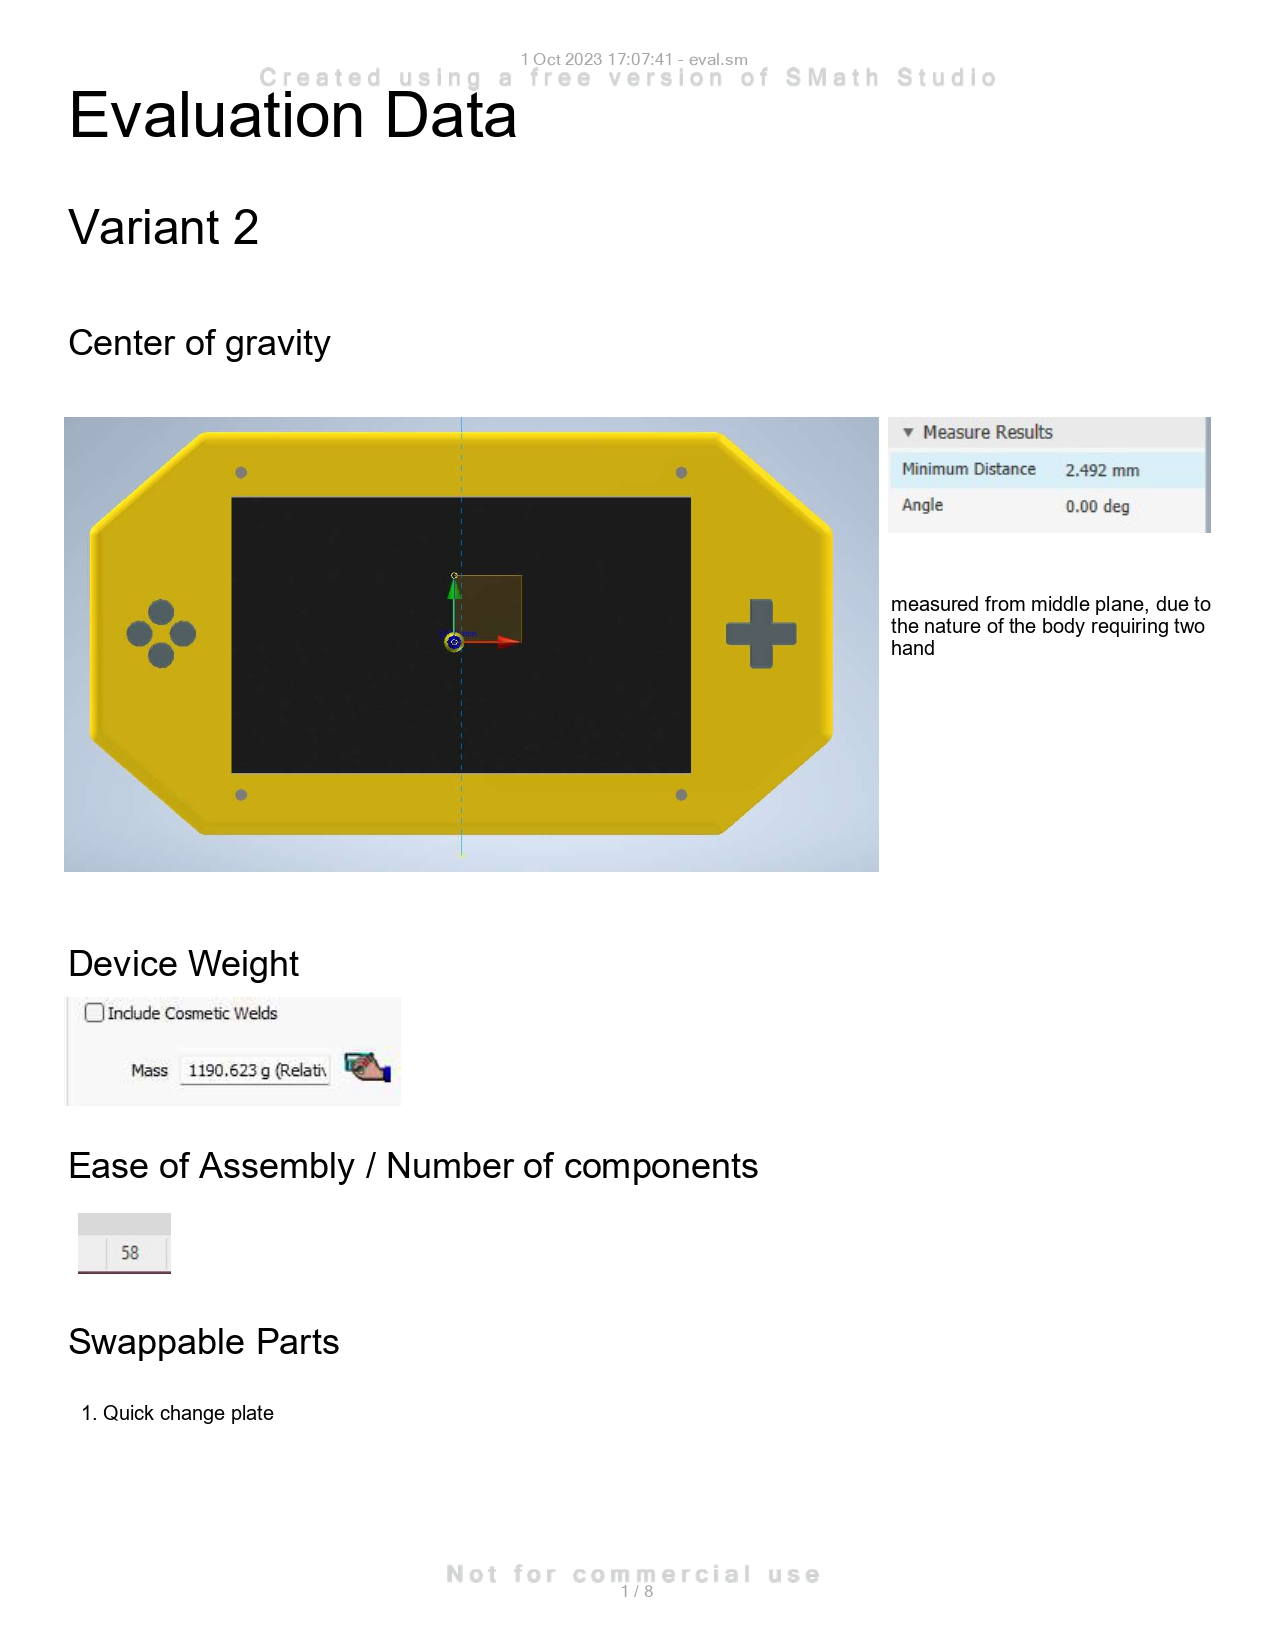
\includegraphics[width=\linewidth]{texs/appendix/data/evaluation/eval_page-0001.jpg}
    \caption{Evaluation 1}
    \label{fig:evaluation-1}
\end{figure}

\begin{figure}[H]
    \centering
    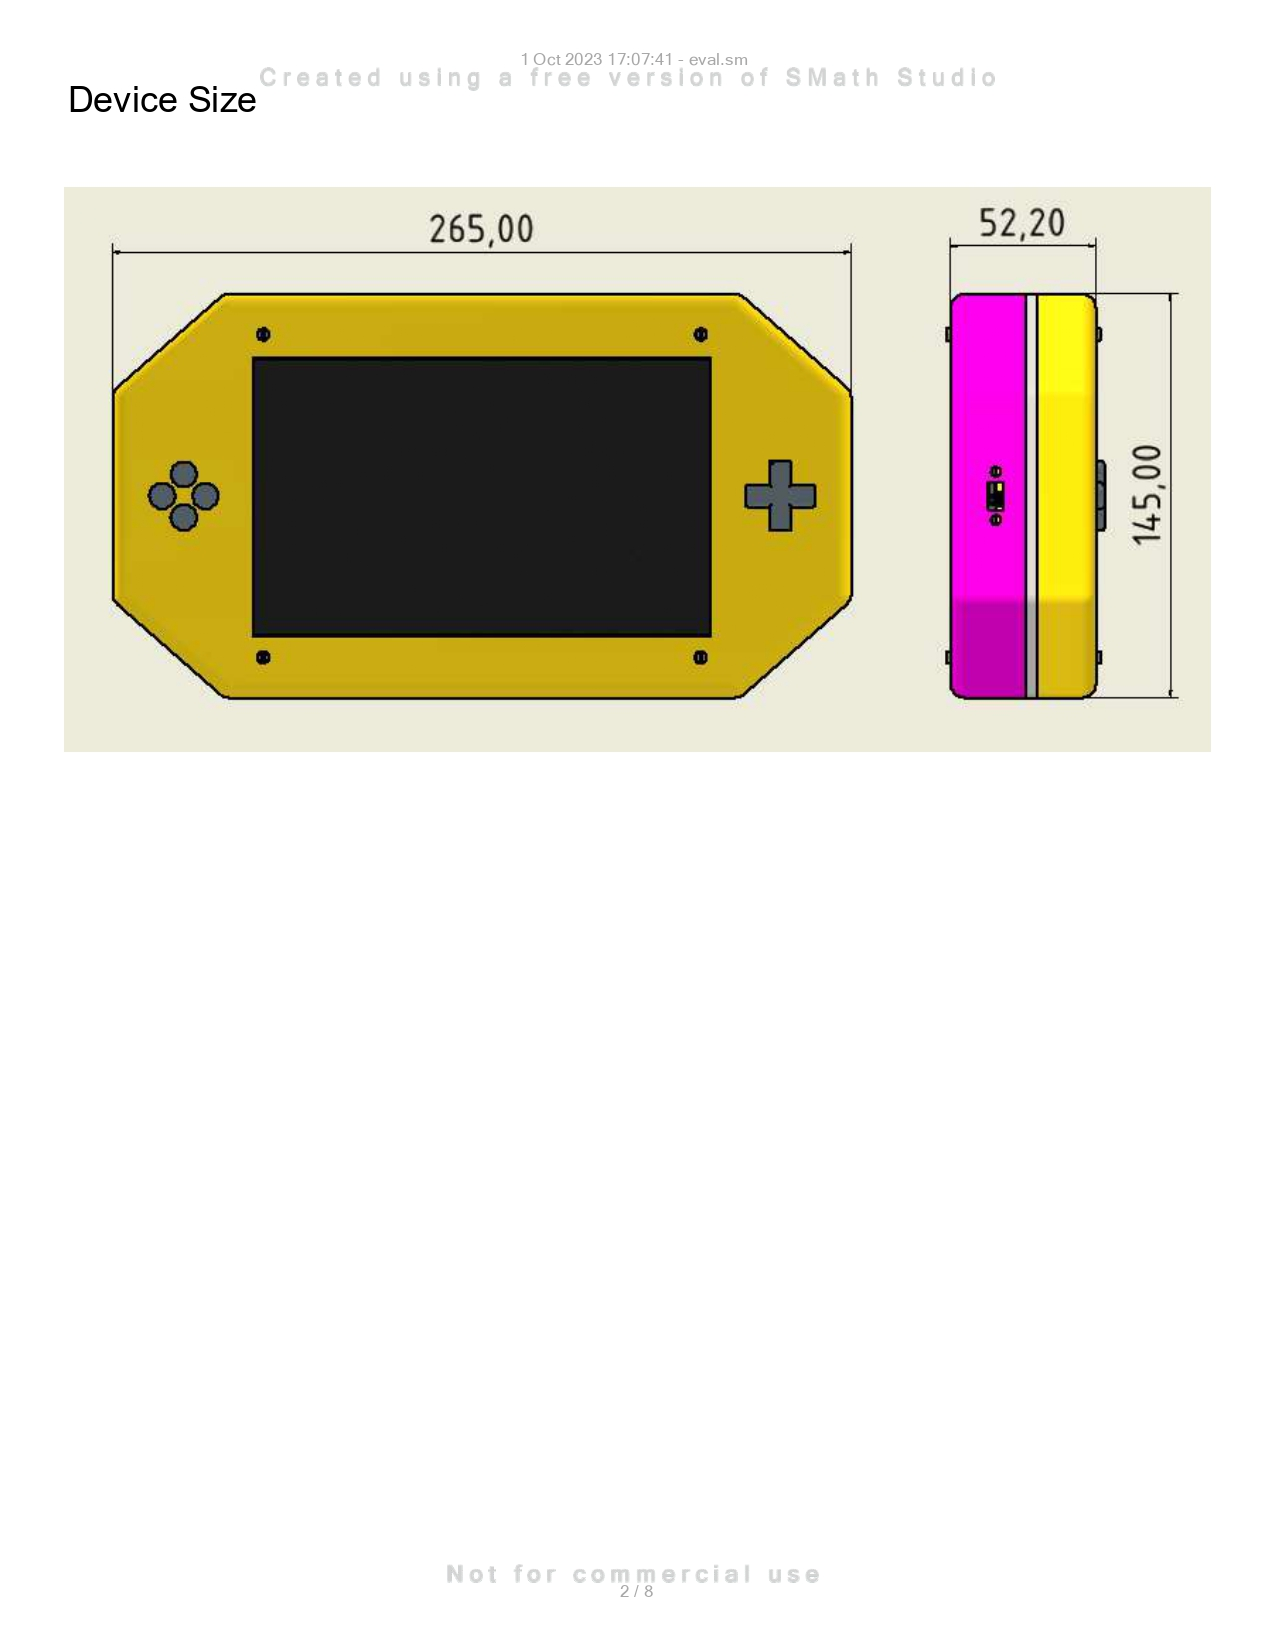
\includegraphics[width=\linewidth]{texs/appendix/data/evaluation/eval_page-0002.jpg}
    \caption{Evaluation 2}
    \label{fig:evaluation-2}
\end{figure}

\begin{figure}[H]
    \centering
    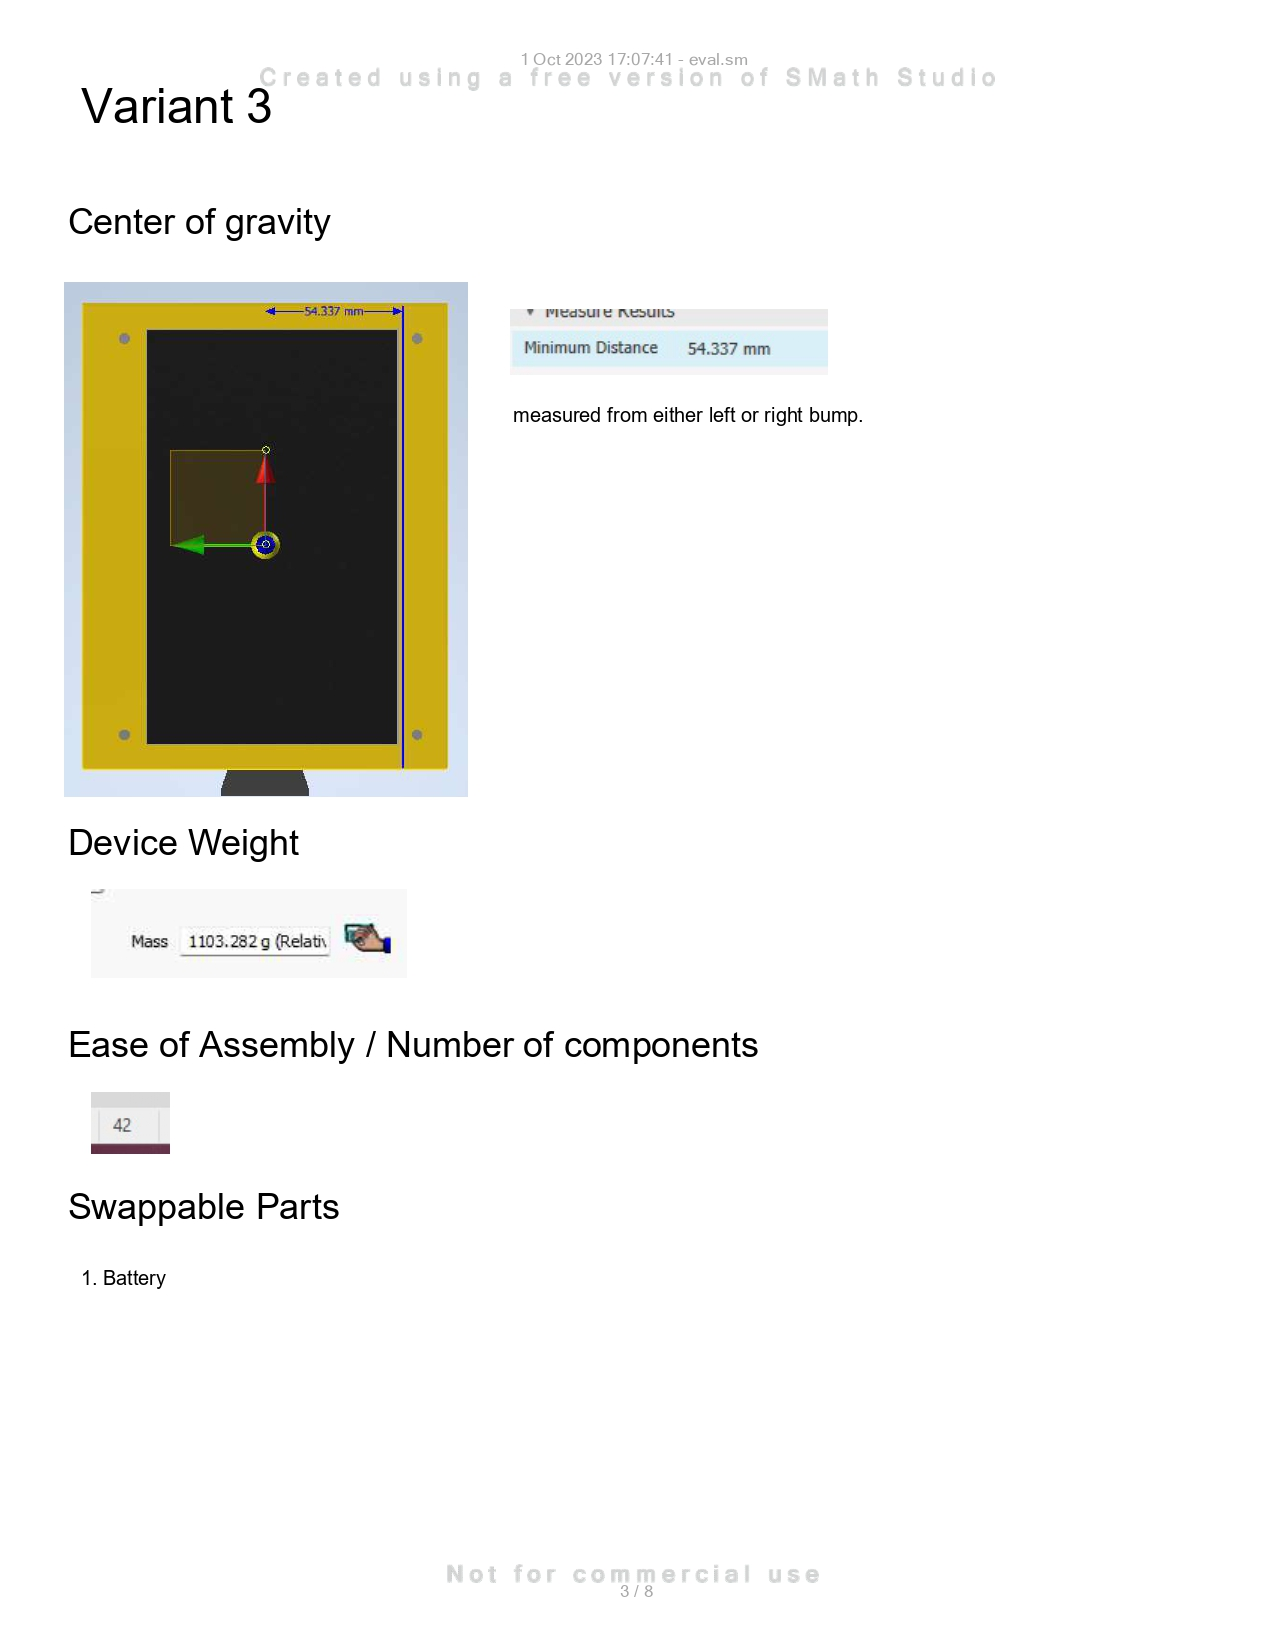
\includegraphics[width=\linewidth]{texs/appendix/data/evaluation/eval_page-0003.jpg}
    \caption{Evaluation 3}
    \label{fig:evaluation-3}
\end{figure}

\begin{figure}[H]
    \centering
    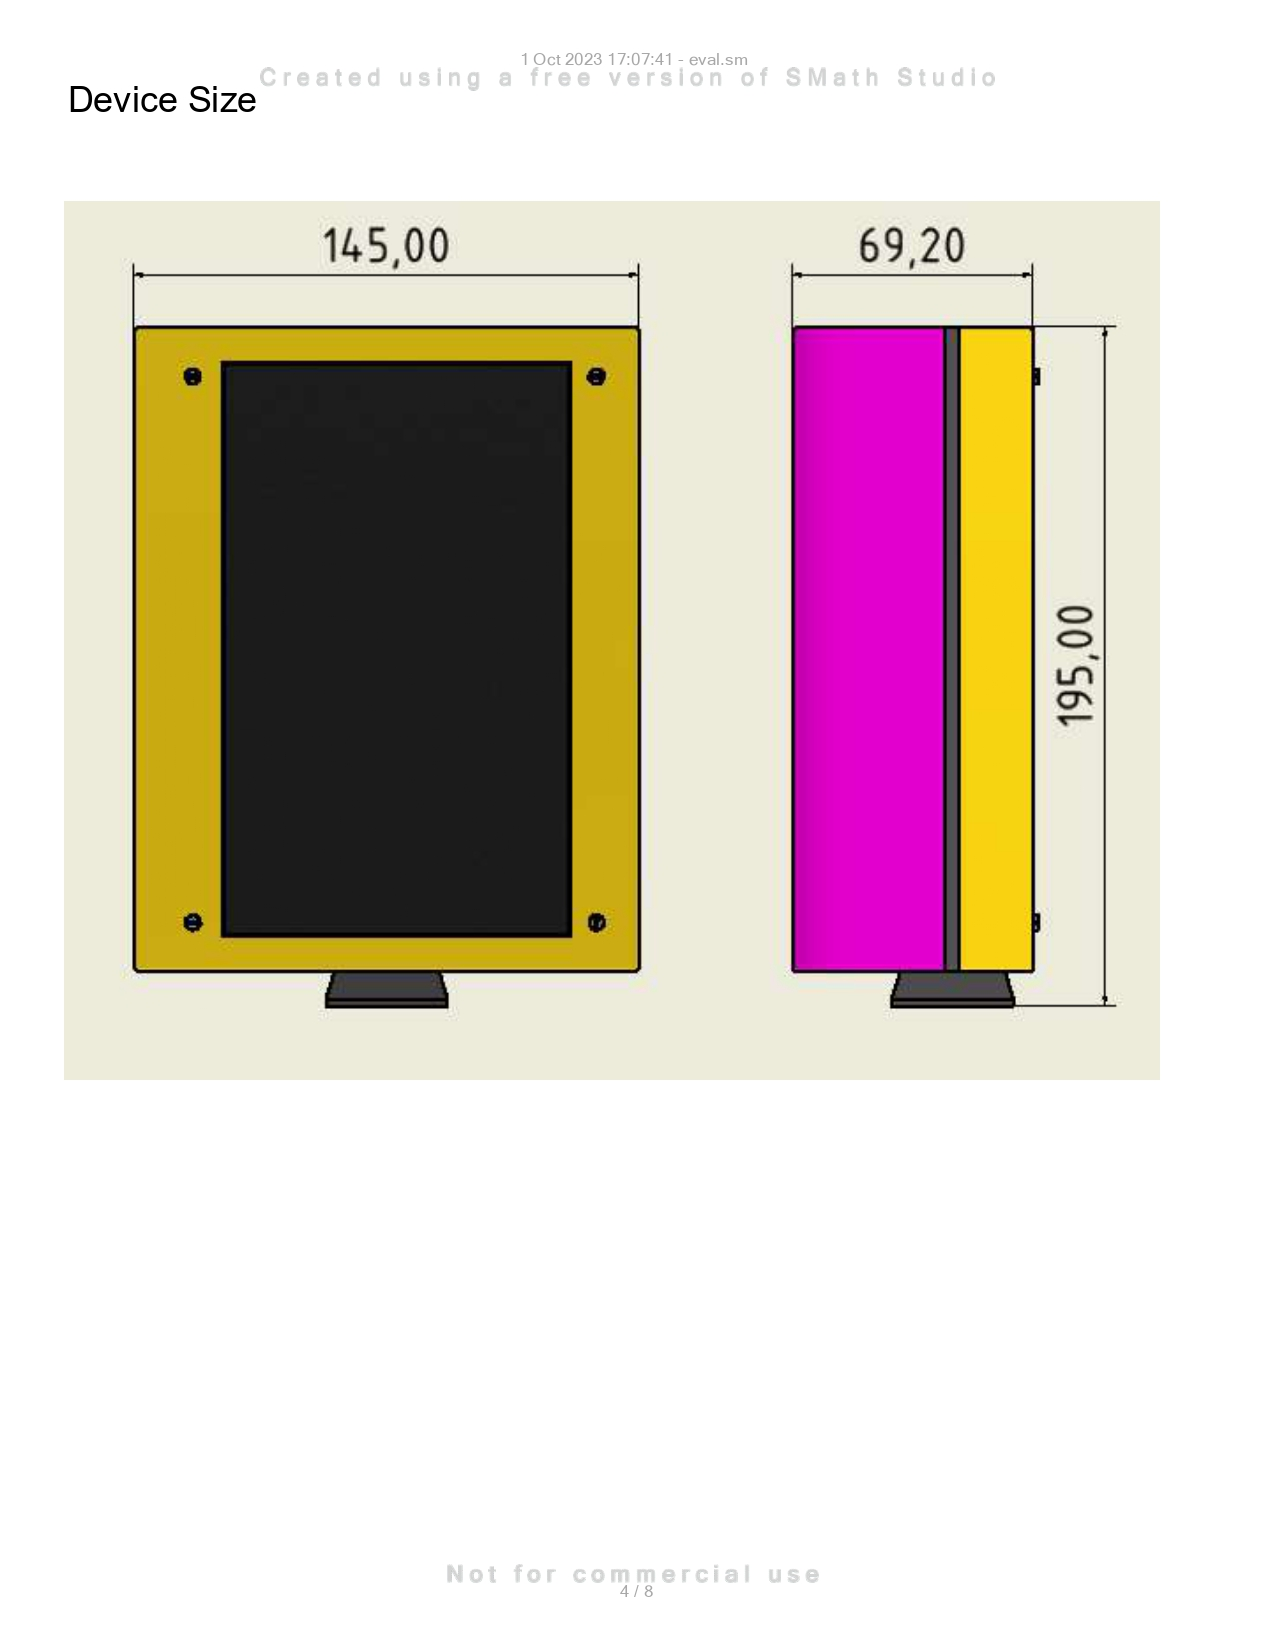
\includegraphics[width=\linewidth]{texs/appendix/data/evaluation/eval_page-0004.jpg}
    \caption{Evaluation 4}
    \label{fig:evaluation-4}
\end{figure}

\begin{figure}[H]
    \centering
    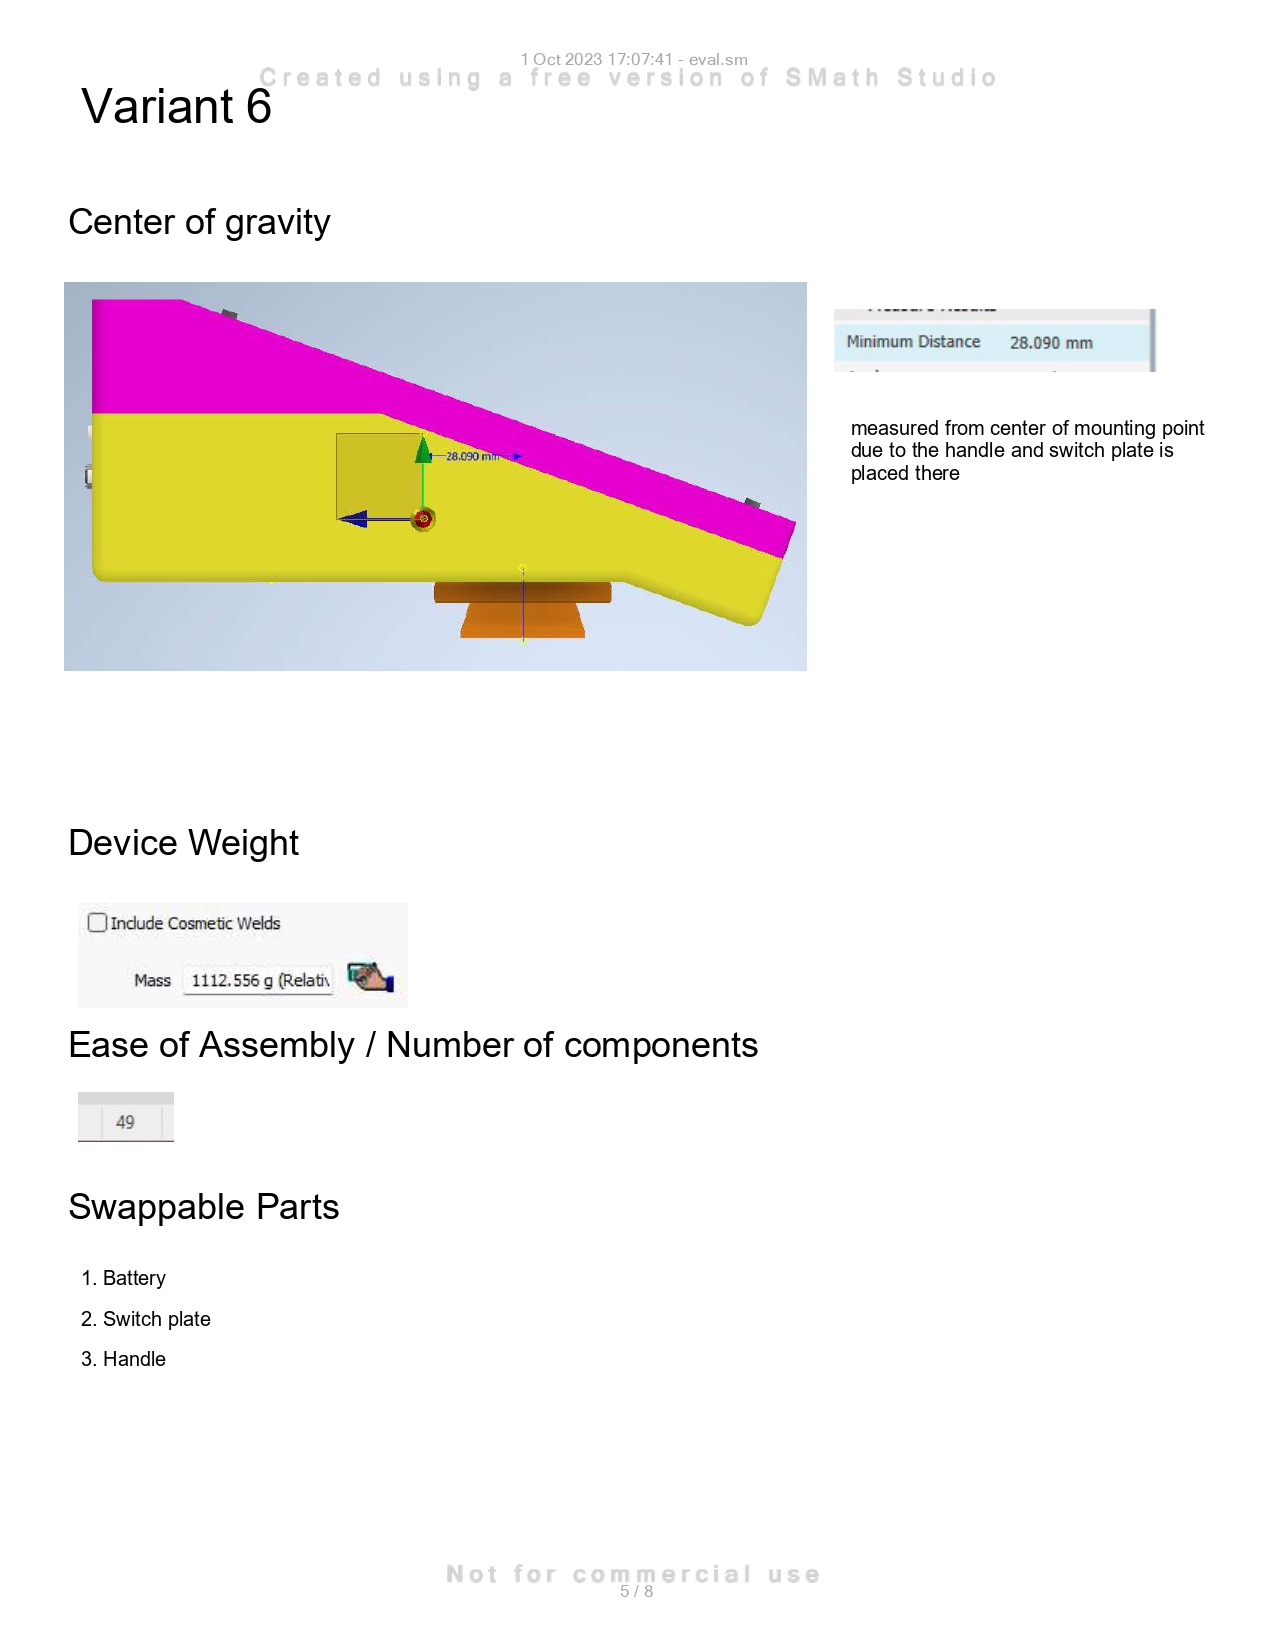
\includegraphics[width=\linewidth]{texs/appendix/data/evaluation/eval_page-0005.jpg}
    \caption{Evaluation 5}
    \label{fig:evaluation-5}
\end{figure}

\begin{figure}[H]
    \centering
    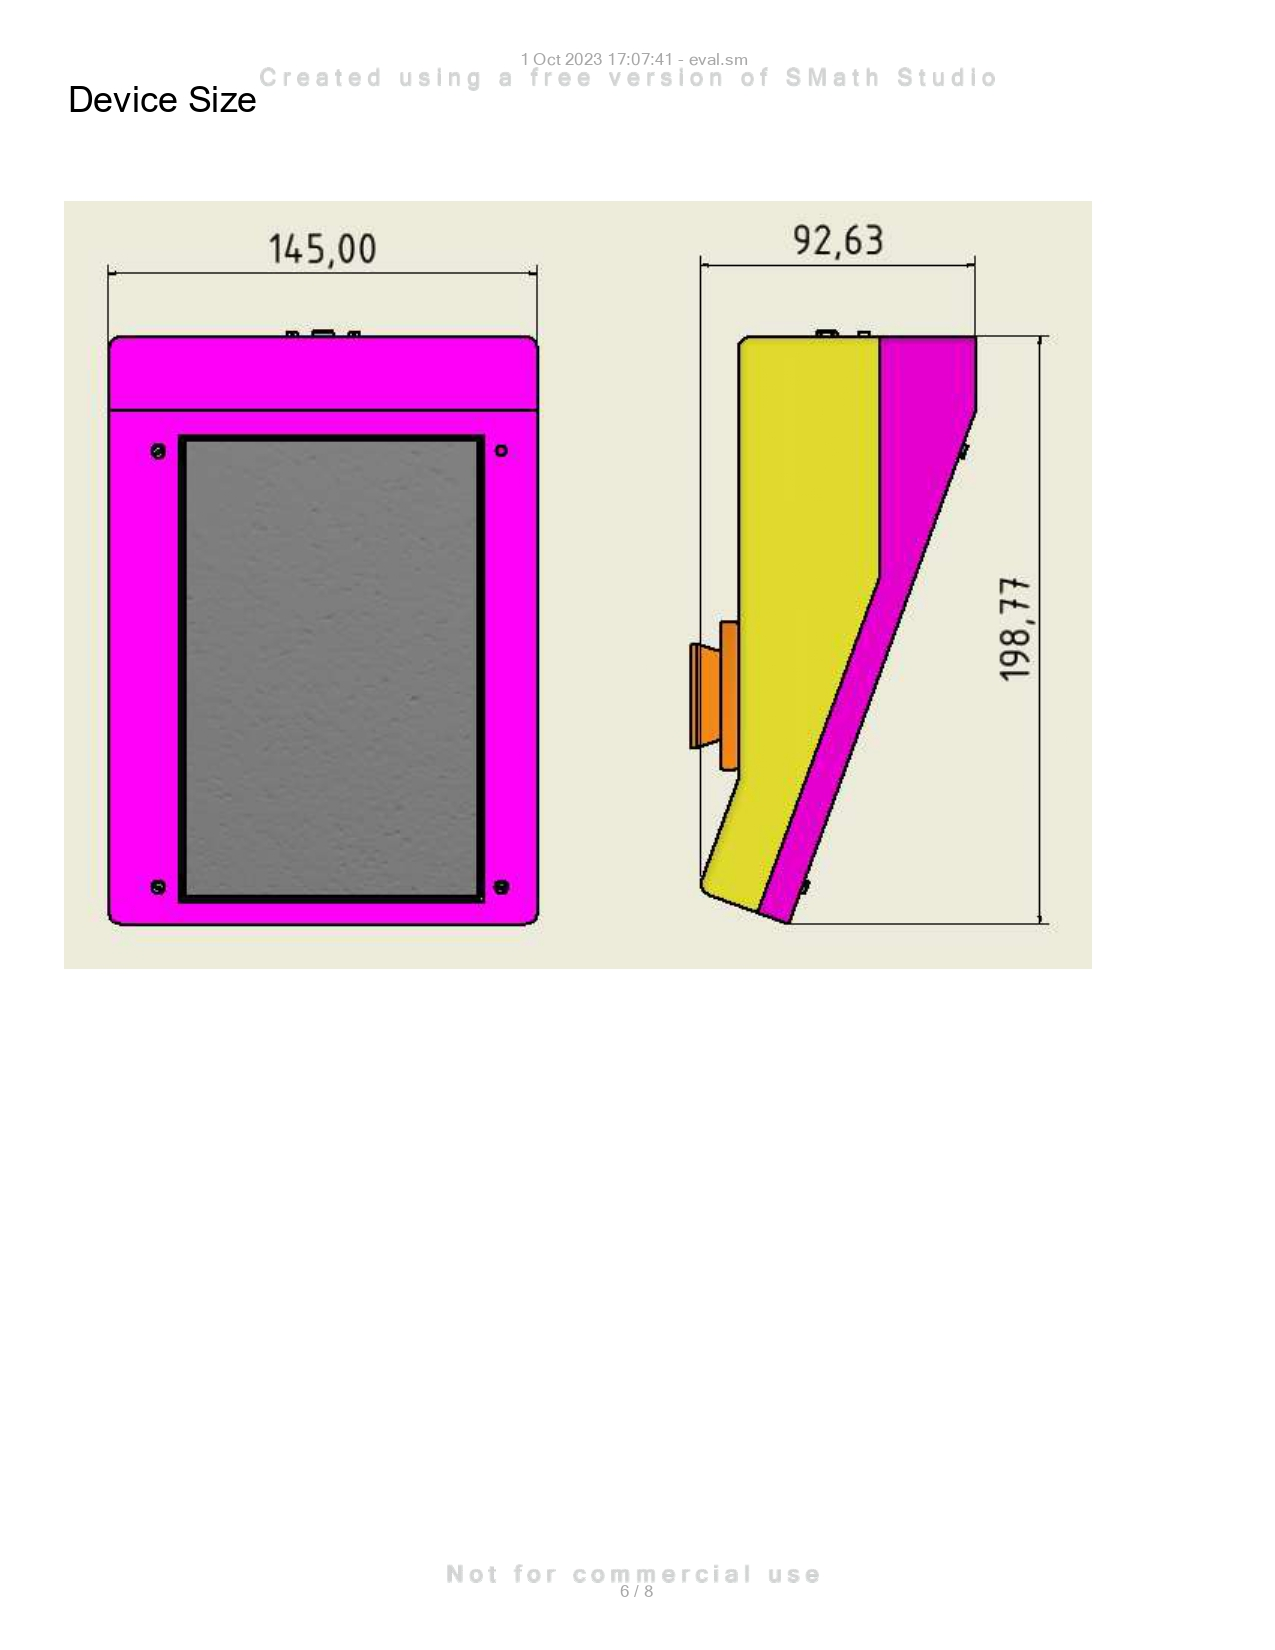
\includegraphics[width=\linewidth]{texs/appendix/data/evaluation/eval_page-0006.jpg}
    \caption{Evaluation 6}
    \label{fig:evaluation-6}
\end{figure}

\begin{figure}[H]
    \centering
    \includegraphics[width=\linewidth]{texs/appendix/data/evaluation/eval_page-0007.jpg}
    \caption{Evaluation 7}
    \label{fig:evaluation-7}
\end{figure}

\begin{figure}[H]
    \centering
    \includegraphics[width=\linewidth]{texs/appendix/data/evaluation/eval_page-0008.jpg}
    \caption{Evaluation 8}
    \label{fig:evaluation-8}
\end{figure}

\section{Project Documentation}
\label{appendix:documentation}

\begin{itemize}
    \item \href{https://github.com/HaziqSabtu/SpeedCameraPi}{Repository}
    \item \href{https://haziqsabtu.github.io/SpeedCameraPi/}{Documentation}
    \item \href{https://drive.google.com/file/d/1rwLjBPgVh4GH8QMI73DD1_Jq8OOce9Yv/view?usp=sharing}{PDF}
\end{itemize}

\section{C++ Unit Tests for Bank Account Management}
\label{appendix:unit-tests}

\subsection*{Bank Account Class}

\begin{lstlisting}[language=C++]
class BankAccount {
private:
    double balance;

public:
    BankAccount() : balance(0.0) {}

    void deposit(double amount) {
        if (amount < 0) {
            throw std::invalid_argument("Deposit amount must be positive");
        }
        balance += amount;
    }

    void withdraw(double amount) {
        if (amount < 0) {
            throw std::invalid_argument("Withdrawal amount must be positive");
        }
        if (amount > balance) {
            throw std::runtime_error("Insufficient funds for withdrawal");
        }
        balance -= amount;
    }

    double getBalance() const {
        return balance;
    }
};
\end{lstlisting}

\subsection*{Unit Tests}

\subsubsection*{Test Case: Deposit}
\begin{lstlisting}[language=C++]
TEST(BankAccountTest, Deposit) {
    BankAccount account;
    account.deposit(100.0);
    EXPECT_EQ(account.getBalance(), 100.0);
}
\end{lstlisting}

\textbf{Explanation:} This test verifies that funds can be successfully deposited into the account. It creates an instance of \texttt{BankAccount}, deposits $100.0$ units, and then checks if the balance matches the expected value of $100.0$.

\subsubsection*{Test Case: Withdraw}
\begin{lstlisting}[language=C++]
TEST(BankAccountTest, Withdraw) {
    BankAccount account;
    account.deposit(100.0);
    account.withdraw(50.0);
    EXPECT_EQ(account.getBalance(), 50.0);
}
\end{lstlisting}

\textbf{Explanation:} This test ensures that withdrawals are processed correctly. It first deposits $100.0$ units into the account, then attempts to withdraw $50.0$ units. The test verifies if the balance is now $50.0$ units.

\subsubsection*{Test Case: Withdraw Too Much}
\begin{lstlisting}[language=C++]
TEST(BankAccountTest, WithdrawTooMuch) {
    BankAccount account;
    account.deposit(100.0);

    EXPECT_THROW(account.withdraw(150.0), std::runtime_error);
    EXPECT_EQ(account.getBalance(), 100.0);
}
\end{lstlisting}

\textbf{Explanation:} This test examines the scenario where an attempt is made to withdraw an amount greater than the available balance. It first deposits $100.0$ units and then tries to withdraw $150.0$ units. The test expects a \texttt{std::runtime\_error} to be thrown, and ensures that the balance remains unchanged.

\subsubsection*{Test Case: Deposit Negative}
\begin{lstlisting}[language=C++]
TEST(BankAccountTest, DepositNegative) {
    BankAccount account;

    EXPECT_THROW(account.deposit(-50.0), std::invalid_argument);
    EXPECT_EQ(account.getBalance(), 0.0);
}
\end{lstlisting}

\textbf{Explanation:} This test handles the scenario where an attempt is made to deposit a negative amount. It expects a \texttt{std::invalid\_argument} exception to be thrown. The test also verifies that the account balance remains unaffected.


\section{User Manual}
\label{appendix:user-manual}

Also available online at \href{https://drive.google.com/file/d/1CKM41b0lVNlPVhcOHVzftnJ13RWR5m6Y/view?usp=drive_link}{Google Drive}.

\includepdf[pages={1-},scale=0.75]{texs/appendix/data/guide/usermanual.pdf}

\section{Developer Manual}
\label{appendix:developer-manual}

Also available online at \href{https://drive.google.com/file/d/1Dm2La7uIj3iK4M7hl8aNyZqYd4_LneJs/view?usp=sharing}{Google Drive}.

\includepdf[pages={1-},scale=0.75]{texs/appendix/data/guide/developermanual.pdf}